\documentclass[oneside, a4paper, 12pt]{book}
\usepackage[left=3.5cm, right=2.5cm, top=2cm, bottom=2cm]{geometry}

\usepackage{graphicx}
\usepackage{array}
\graphicspath{{figures/}}

\usepackage{indentfirst}
\usepackage{hyperref}
% expansion=false: tránh lỗi "auto expansion is only possible with scalable fonts"
% khi dùng font T5 (gói vietnam) + Times/mathptmx trên Overleaf/MiKTeX
\usepackage[protrusion=true,expansion=false]{microtype}
\usepackage{pdfpages}
\usepackage{lmodern}
\usepackage{multirow}
\usepackage{cite}
\usepackage{enumitem}
\usepackage{float}
\usepackage{wrapfig}
\usepackage{tikz}
\usetikzlibrary{patterns}
\usepackage{subcaption}
\usepackage{listings}
\usepackage{xcolor}
\usepackage{booktabs}
\usepackage{setspace}

\definecolor{codegreen}{rgb}{0,0.6,0}
\definecolor{codegray}{rgb}{0.5,0.5,0.5}
\definecolor{codepurple}{rgb}{0.58,0,0.82}
\definecolor{backcolour}{rgb}{0.95,0.95,0.92}
\definecolor{figboxborder}{rgb}{0.45,0.50,0.55}
\definecolor{figboxbg}{rgb}{0.96,0.97,0.98}
\definecolor{figboxhint}{rgb}{0.25,0.30,0.35}

\lstdefinestyle{mystyle}{
	backgroundcolor=\color{backcolour},
	commentstyle=\color{codegreen},
	keywordstyle=\color{magenta},
	numberstyle=\tiny\color{codegray},
	stringstyle=\color{codepurple},
	basicstyle=\ttfamily\footnotesize,
	breakatwhitespace=false,
	breaklines=true,
	captionpos=b,
	keepspaces=true,
	numbers=left,
	numbersep=5pt,
	showspaces=false,
	showstringspaces=false,
	showtabs=false,
	tabsize=2
}
\lstset{style=mystyle}

\usepackage{amsmath,amssymb,latexsym,amscd,amsxtra,amsthm}
\usepackage{mathtools}
\usepackage{mathptmx}
\usepackage{indentfirst}
\usepackage{caption}
\usepackage{aligned-overset}
\usepackage{longtable}
\usepackage{fancybox}
\usepackage[utf8]{vietnam}
\usepackage[tight,vietnam]{minitoc}
\usepackage{anyfontsize}

%==================================
\usepackage{titletoc}
\titlecontents{chapter}
  [0pt]
  {\bfseries}
  {\chaptername\ \thecontentslabel\enskip}
  {}
  {\hfill\contentspage}

%==================================
\renewcommand{\thechapter}{\arabic{chapter}}
\renewcommand{\thesection}{\arabic{chapter}.\arabic{section}}
\newcommand{\eproof}{\hfill $\square$}
\newcommand{\chm}{{\bfseries Chứng minh.}}
\newenvironment{cm}{\chm}{\eproof}

\theoremstyle{plain}
\newtheorem{bd}{Bổ đề}[chapter]
\providecommand*{\bdautorefname}{Bổ đề}
\newtheorem{md}{Mệnh đề}[chapter]
\providecommand*{\mdautorefname}{Mệnh đề}
\newtheorem{hq}{Hệ quả}[chapter]
\providecommand*{\hqautorefname}{Hệ quả}
\newtheorem{dl}{\bfseries Định lý}[chapter]
\providecommand*{\dlautorefname}{Định lý}
\newtheorem{algorithm}{\bfseries Thuật toán}[chapter]
\providecommand*{\algorithmautorefname}{Thuật toán}
\newtheorem{gt}{\bfseries Giả thiết}[chapter]
\providecommand*{\gtautorefname}{Giả thiết}
\newtheorem{algorithmm}{Thuật toán}[chapter]
\providecommand*{\algorithmmautorefname}{Thuật toán}

\newtheorem*{namedthm}{\namedthmname}
\newcounter{namedthm}
\makeatletter
\newenvironment{named}[1]
  {\def\namedthmname{#1}%
   \refstepcounter{namedthm}%
   \namedthm\def\@currentlabel{#1}}
  {\endnamedthm}
\makeatother

\theoremstyle{definition}
\newtheorem{dn}{Định nghĩa}[chapter]
\providecommand*{\dnautorefname}{Định nghĩa}
\newtheorem{bt}{Bài toán}[chapter]
\providecommand*{\btautorefname}{Bài toán}
\newtheorem{vd}{\bfseries Ví dụ}[chapter]
\providecommand*{\vdautorefname}{Ví dụ}

\theoremstyle{remark}
\newtheorem{kh}{Ký hiệu}[chapter]
\newtheorem{nx}{\bfseries Nhận xét}[chapter]
\newtheorem{cy}{Chú ý}[chapter]

%------------------------------------------------------------------------------
% Placeholder hình ảnh --- bổ sung file sau, giữ nguyên caption/label
% Cách dùng: \figtodo{nhan}{Chú thích}{Mô tả nội dung cần vẽ/chụp}{ten_file}
% Tùy chọn chiều cao: \figtodo[0.32\textheight]{nhan}{...}{...}{...}
%------------------------------------------------------------------------------
\newcommand{\figtodo}[5][0.28\textheight]{%
  \begin{figure}[htbp]
    \centering
    \fcolorbox{figboxborder}{figboxbg}{%
      \begin{minipage}[c][#1][c]{0.92\textwidth}
        \centering
        \color{figboxhint}
        {\small\bfseries [Chỗ chèn hình --- bổ sung sau]}\\[0.55em]
        {\scriptsize\bfseries Nội dung hình cần thể hiện:}\\[0.3em]
        {\footnotesize\itshape #4}\\[0.65em]
        {\scriptsize\ttfamily Tên file đề xuất: figures/{\detokenize{#5}}}\\[0.2em]
        {\scriptsize Nguồn gợi ý: sơ đồ (Draw.io/PowerPoint/TikZ),
          ảnh piano-roll, hoặc biểu đồ từ \texttt{compare/results}.}\\[0.15em]
        {\scriptsize Khi đã có file: thay khung bằng
          \texttt{\string\includegraphics}.}
      \end{minipage}%
    }%
    \caption{#3}
    \label{#2}
  \end{figure}%
}

% Debug figtodo
\renewcommand{\figtodo}[5][0.28\textheight]{%
  \begin{figure}[htbp]
    \centering
    \fbox{\parbox{0.9\textwidth}{\small [PLACEHOLDER: #4]}}
    \caption{#3}
    \label{#2}
  \end{figure}
}

\renewcommand{\baselinestretch}{1.5}
\setlength{\oddsidemargin}{0.3cm}
\setlength{\topmargin}{-1cm}
\setlength{\headsep}{0.5cm}
\textwidth=15.5cm
\textheight=24.5cm
\renewcommand{\bibname}{Tài liệu tham khảo}
\renewcommand{\large}{\fontsize{14pt}{14pt}\selectfont}
\renewcommand{\Large}{\fontsize{16pt}{16pt}\selectfont}
\renewcommand{\LARGE}{\fontsize{15pt}{15pt}\selectfont}
\renewcommand{\th}{\fontsize{18pt}{18pt}\selectfont}

\pagestyle{myheadings}
\usepackage{fancyhdr}
\fancyhf{}
\rfoot{\thepage\quad\ }
\pagestyle{fancy}
\fancypagestyle{plain}{
  \fancyhf{}
  \rfoot{\thepage\quad\ }
  \renewcommand{\headrulewidth}{0pt}
}
\renewcommand{\headrulewidth}{0pt}

\newenvironment{mproof}{\paragraph{Chứng minh:}}{\hfill$\square$}
\newenvironment{myproof}[2]{\paragraph{Proof of {#1} {#2}:}}{\hfill$\square$}
\DeclarePairedDelimiter{\pro}{\langle}{\rangle}
\DeclarePairedDelimiter{\norm}{\lVert}{\rVert}
\DeclarePairedDelimiter{\abs}{\lvert}{\rvert}
\usepackage{xpatch}
\makeatletter
\AtBeginDocument{\xpatchcmd{\@thm}{\thm@headpunct{.}}{\thm@headpunct{}}{}{}}
\makeatother
\DeclareMathOperator{\vip}{VIP}
\DeclareMathOperator{\svip}{SVIP}
\DeclareMathOperator{\fix}{Fix}
\allowdisplaybreaks

% Hyperref setup (đặt sau các package khác)
\hypersetup{
  colorlinks=true,
  linkcolor=black,
  citecolor=black,
  urlcolor=blue,
  pdftitle={So sánh Music Transformer và Piano-roll Diffusion trong bài toán sinh nhạc},
  pdfauthor={Nhóm sinh viên Đồ án tốt nghiệp}
}

\begin{document}

\thispagestyle{empty}
\setcounter{page}{1}
\pagenumbering{roman}
\pagenumbering{gobble}
\newgeometry{left=3.5cm,right=2.5cm,top=2cm,bottom=2cm}

\begin{center}
\Large
\vspace{-1cm}
{\bfseries ĐẠI HỌC BÁCH KHOA HÀ NỘI}\\
{\bfseries KHOA TOÁN -- TIN}
\end{center}
\vspace{4.5cm}
\begin{center}
    \fontsize{20pt}{16pt}\selectfont
	{\bfseries ĐỒ ÁN TỐT NGHIỆP}\\
	\fontsize{17pt}{15pt}\selectfont
	
\includegraphics[scale=0.08]{HUST_logo}\\
	\vspace{1.25cm}
	\fontsize{18pt}{20pt}\selectfont
	\bfseries So sánh Music Transformer và Piano-roll Diffusion\\
	trong bài toán sinh nhạc có điều kiện
\end{center}
\vspace{1cm}
\begin{center}
\fontsize{12pt}{14pt}\selectfont
\begin{tabular}{ll}
\textbf{PHẠM TUẤN ANH} & MSSV: 20195840 \\
\textbf{TRẦN BÁ ĐẠT} & MSSV: \rule{3cm}{0.4pt} \\
\textbf{NGUYỄN KHÁNH TRƯỜNG LỘC} & MSSV: \rule{3cm}{0.4pt} \\
\textbf{PHẠM ĐÀM QUÂN} & MSSV: \rule{3cm}{0.4pt} \\
\textbf{VŨ ĐỨC MINH} & MSSV: \rule{3cm}{0.4pt}
\end{tabular}
\vspace{0.6cm}
\end{center}
\vspace{2cm}
\begin{center}
\fontsize{13pt}{16pt}\selectfont
\textbf{\begin{tabular}{l l}
Giảng viên hướng dẫn:& \textmd{TS.\ Trịnh Văn Chiến $\underset{\text{Chữ ký của GVHD}}{\rule{3cm}{0.5pt}}$}\\
\end{tabular}}
\end{center}
\vspace{2.5cm}
\begin{center}
\LARGE \textbf{HÀ NỘI, 07/2026}
\end{center}


\newpage
\thispagestyle{empty}
\newgeometry{left=3cm,right=2.8cm,top=2cm,bottom=2cm}
\setcounter{page}{1}
\thisfancypage{
	\setlength{\fboxsep}{0.5cm}
	\fbox}{}

\fontsize{13pt}{16pt}\selectfont
\bigbreak
\begin{center}
	{\bfseries NHẬN XÉT CỦA GIẢNG VIÊN HƯỚNG DẪN}
\end{center}
\bigbreak

\fontsize{12pt}{14pt}\selectfont
\begin{enumerate}
	\item [{\bfseries 1.}]{\bfseries Mục tiêu và nội dung của đồ án}
	\begin{enumerate}
		\item Mục tiêu:
		\item Nội dung:
	\end{enumerate}
	\item [{\bfseries 2.}] {\bfseries Kết quả đạt được}
	\begin{enumerate}
		\item
		\item
	\end{enumerate}
	\item [{\bfseries 3.}]{\bfseries Ý thức làm việc của sinh viên:}
\begin{enumerate}
	\item
	\item
	\item
\end{enumerate}
\end{enumerate}
\hspace{0.5\textwidth}
\begin{minipage}{0.5\textwidth}
	\noindent\begin{center}
		\textit{Hà Nội, tháng \ldots\ năm 2026} \\
		Giảng viên hướng dẫn\\ \vspace{2cm}
		\textbf{TS.\ Trịnh Văn Chiến}
	\end{center}
\end{minipage}
\restoregeometry


\newpage
\restoregeometry

\newpage
\fontsize{16pt}{18pt}\selectfont
\thispagestyle{empty}

{\bfseries Tóm tắt nội dung báo cáo}
\fontsize{12pt}{16pt}\selectfont
\bigskip

Báo cáo nghiên cứu bài toán sinh nhạc nền có điều kiện dưới dạng MIDI. Điều kiện được tổ chức theo \textbf{hai tầng}: (i)~sáu thuộc tính rời rạc (\textit{mood}, \textit{genre}, \textit{scene}, \textit{tempo}, \textit{instrument}, \textit{energy}) dùng để gán nhãn dữ liệu, xây chú thích huấn luyện và tính chỉ số đánh giá; (ii)~một câu mô tả tiếng Anh đưa vào mô hình qua bộ mã hóa ngôn ngữ nhẹ \texttt{all-MiniLM-L6-v2} (đóng băng) kèm lớp chiếu học được --- cùng lớp mã nguồn dùng chung cho cả hai nhánh (mỗi nhánh vẫn huấn luyện projection riêng). Khi huấn luyện, câu thường được ghép theo mẫu từ sáu nhãn; khi suy luận/đánh giá có thể dùng câu viết sẵn hoặc câu ghép. Trọng tâm là \textbf{triển khai và so sánh có kiểm soát} hai họ kiến trúc tạo sinh: \textit{Music Transformer} (tự hồi quy trên chuỗi token sự kiện kiểu REMI) và \textit{Piano-roll Diffusion} (khuếch tán trên lưới cao độ--thời gian), trên cùng kho dữ liệu, cùng phân chia huấn luyện/kiểm định và cùng giao thức đánh giá.

Hệ thống được hiện thực hóa theo quy trình đầu cuối (\textit{end-to-end}) bằng PyTorch. Nhánh Transformer sử dụng cơ chế chú ý chéo (\textit{cross-attention}) trên vector điều kiện từ câu văn bản và huấn luyện bằng hàm mất mát entropy chéo (\textit{cross-entropy}) có làm mượt nhãn. Nhánh Diffusion sử dụng UNet điều chế FiLM, lịch nhiễu cosine, hướng dẫn không dùng bộ phân loại (\textit{classifier-free guidance}, CFG), trung bình trượt tham số (EMA) và lấy mẫu DDIM. Kho dữ liệu đã xử lý gồm khoảng 14\,232 tệp MIDI (12\,809 mẫu huấn luyện / 1\,423 mẫu kiểm định). Thực nghiệm 30 epoch trên GPU RTX~3060 cho thấy cả hai nhánh hội tụ ổn định trên hàm mục tiêu riêng (entropy chéo kiểm định $\approx 2{,}39$, độ bối rối $\approx 10{,}9$ với Transformer; sai số bình phương trung bình kiểm định $\approx 0{,}0029$ với Diffusion). Về các chỉ số cấu trúc MIDI, Transformer cho mật độ nốt và đa âm ở mức thưa hơn, đồng thời chỉ số khớp nhạc cụ tăng theo quá trình học (tới $\approx 0{,}37$); Diffusion đạt MSE thấp nhưng mật độ và đa âm rất cao, trong khi chỉ số khớp nhạc cụ bằng $1{,}0$ gắn với việc gán chương trình nhạc cụ (\textit{program}) theo nhãn instrument khi giải mã, không phản ánh thuần túy việc học âm sắc (\textit{timbre}).

Báo cáo không khẳng định vượt các hệ text-to-audio quy mô lớn. Đóng góp chính gồm quy trình so sánh thống nhất (kèm đặc tả điều kiện text dùng chung), phân tích liên kết giữa thiết kế triển khai và kết quả đo được (bao gồm các hạn chế khi diễn giải chỉ số), cùng các nhận định về sự đánh đổi phương pháp dựa trên số liệu thực nghiệm.

Báo cáo gồm bốn chương: giới thiệu; cơ sở lý thuyết và công trình liên quan; triển khai hệ thống; kết quả thực nghiệm và đánh giá --- kèm phần kết luận.

\tableofcontents

\newpage

\thispagestyle{fancy}
\pagenumbering{arabic}
\setcounter{page}{1}

\chapter{Giới thiệu}
\label{chap:intro}

Sự phát triển mạnh của các mô hình tạo sinh (\textit{generative models}) trong những năm gần đây không chỉ thay đổi cách máy tính sinh văn bản hay hình ảnh, mà còn mở rộng sang các miền đa phương thức khác, trong đó có âm nhạc. Trong công nghiệp game và truyền thông tương tác, nhu cầu nhạc nền (\textit{background music} --- BGM) gắn với ngữ cảnh cụ thể --- ví dụ không gian làng yên tĩnh, trận chiến căng thẳng, hoặc bối cảnh giả tưởng --- ngày càng tăng, trong khi chi phí thuê nhạc sĩ chuyên nghiệp thường vượt khả năng của nhiều nhóm phát triển quy mô nhỏ. Trong bối cảnh đó, bài toán \textbf{sinh nhạc có điều kiện từ mô tả} trở thành hướng nghiên cứu vừa có ý nghĩa thực tiễn, vừa phù hợp để khảo sát các họ kiến trúc tạo sinh khác nhau trên cùng một bài toán có thể kiểm soát.

Báo cáo này không hướng tới xây dựng hệ thống thương mại quy mô lớn hay tái hiện các mô hình audio tiên tiến nhất. Trọng tâm là \textbf{triển khai và so sánh có kiểm soát} hai hướng sinh MIDI phổ biến trong học sâu: mô hình tự hồi quy dựa trên Transformer và mô hình khuếch tán trên piano-roll. Chương này đặt bối cảnh, phát biểu bài toán, nêu mục tiêu cùng các câu hỏi nghiên cứu, đồng thời khoanh phạm vi và đóng góp để các chương sau triển khai và đánh giá một cách nhất quán.

%------------------------------------------------------------------------------
\section{Bối cảnh và động lực}
\label{sec:ch1-motivation}

Trong quy trình sản xuất game, nhạc nền không chỉ đóng vai trò trang trí mà còn điều hướng cảm xúc và nhịp độ trải nghiệm. Cùng một khu vực, người chơi có thể cần đoạn nhạc êm khi khám phá, rồi chuyển sang nhạc dồn dập hơn khi vào trận chiến. Ngay trong cùng thể loại (ví dụ fantasy), nhạc cho cảnh làng yên tĩnh và nhạc cho cảnh hầm ngục căng thẳng thường khác nhau về mật độ nốt, cao độ trung bình và màu sắc nhạc cụ. Việc chuẩn bị thủ công toàn bộ các biến thể này tốn kém về thời gian và nhân lực. Một công cụ sinh nhạc tự động mà vẫn \textit{kiểm soát được} theo các trục như cảm xúc, bối cảnh và nhạc cụ có tiềm năng hỗ trợ nguyên mẫu nhanh, gợi ý ý tưởng, hoặc tạo lớp BGM dự phòng trong giai đoạn tiền sản xuất.

Về mặt kỹ thuật, sinh nhạc khác bài toán phân loại ảnh hay hồi quy một giá trị vô hướng: với cùng một mô tả, có thể tồn tại nhiều bản MIDI hợp lệ, không có đáp án duy nhất. Mô hình cần học cách tạo nốt, nhịp và hòa âm có cấu trúc hợp lý, đồng thời mỗi lần lấy mẫu vẫn có thể cho biến thể khác nhau. Muốn vậy, mô hình thường học một phân phối có điều kiện rồi lấy mẫu từ phân phối đó, thay vì ánh xạ một--một từ nhãn sang đầu ra. Việc chọn kiến trúc kéo theo các giả định khác nhau. Cụ thể, tự hồi quy trên chuỗi sự kiện rời rạc (họ Transformer) và khuếch tán trên biểu diễn liên tục (họ Diffusion) khác nhau về không gian đầu ra, hàm mất mát, và cách đưa điều kiện (prompt) vào mô hình.

Động lực thứ hai mang tính phương pháp luận. Trong học phần và tài liệu về AI tạo sinh, Transformer (kèm các kỹ thuật lấy mẫu chuỗi) và Diffusion (kèm lịch nhiễu, CFG, DDIM) thường được trình bày như hai họ riêng biệt. Người học dễ nắm công thức từng họ, nhưng ít khi quan sát \textbf{cùng một bài toán, cùng một tập dữ liệu và cùng giao thức đánh giá} khi hai họ được hiện thực hóa theo quy trình đầu cuối. Thiếu một khung so sánh như vậy khiến việc bàn luận ưu--nhược điểm dễ rơi vào cảm tính hoặc dựa trên kết quả ở thang đo và miền dữ liệu không tương thích (ví dụ so sánh trực tiếp hàm mất mát của mô hình ngôn ngữ với MSE khử nhiễu, hoặc so sánh sự kiện MIDI với dạng sóng âm thanh).

Tóm lại, báo cáo xây dựng một thực nghiệm so sánh \textit{thống nhất} trong phạm vi khả thi của đồ án tốt nghiệp: dùng MIDI thay vì tín hiệu âm thanh thô (\textit{raw audio}) để giảm chi phí tính toán; dùng \textbf{câu mô tả tiếng Anh} làm đầu vào mô hình (sinh từ nhãn có cấu trúc khi huấn luyện, hoặc nhập trực tiếp khi suy luận) kèm encoder ngôn ngữ nhẹ đóng băng để hai nhánh nhận cùng không gian điều kiện; và đo lường cả chất lượng cấu trúc MIDI lẫn chi phí huấn luyện/suy luận. Cách tiếp cận này chấp nhận đánh đổi mức độ chân thực nghe được so với các hệ audio quy mô lớn, đổi lấy khả năng phân tích sâu phần triển khai và kết quả trên cùng giao thức.

\begin{figure}[htbp]
    \centering
    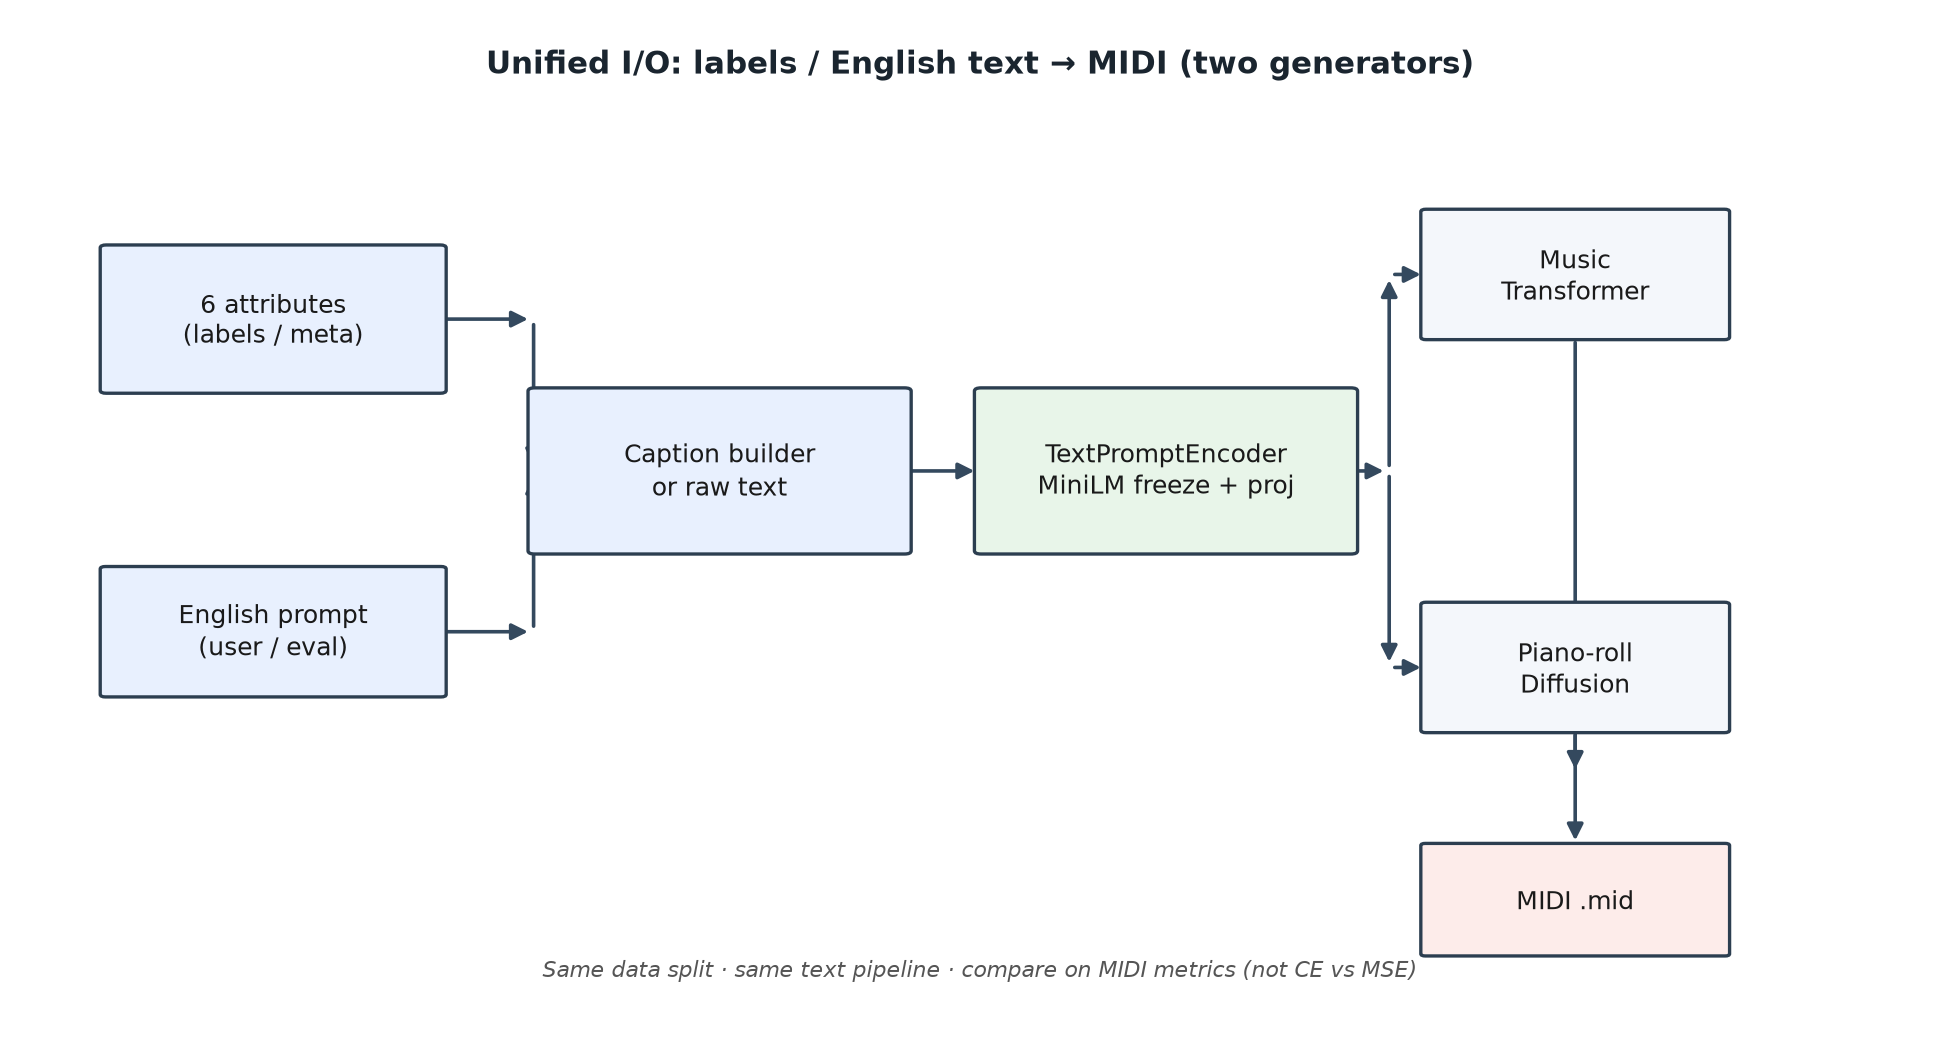
\includegraphics[width=0.95\textwidth]{system_overview_text}
    \caption{Tổng quan bài toán sinh MIDI có điều kiện: nhãn/câu English $\rightarrow$
    MiniLM đóng băng + projection $\rightarrow$ hai nhánh Music Transformer và
    Piano-roll Diffusion $\rightarrow$ tệp MIDI, so sánh bằng chỉ số cấu trúc MIDI.}
    \label{fig:ch1-pipeline-overview}
\end{figure}

%------------------------------------------------------------------------------
\section{Phát biểu bài toán}
\label{sec:ch1-problem}

Bài toán được nghiên cứu có thể phát biểu như sau. Cho một mô tả điều khiển mang ngữ nghĩa âm nhạc--game, hệ thống cần sinh ra một đoạn nhạc dưới dạng tệp MIDI, phản ánh mô tả đó ở mức khả dĩ về mặt thống kê và cấu trúc.

Điều kiện được tổ chức theo \textbf{hai tầng} bổ sung cho nhau.

\paragraph{Tầng ngữ nghĩa có cấu trúc (nhãn).}
Sáu thuộc tính rời rạc theo lớp (\textit{categorical}) được giữ làm lược đồ gán nhãn và siêu dữ liệu:

\begin{center}
\textit{mood}, \textit{genre}, \textit{scene}, \textit{tempo}, \textit{instrument}, \textit{energy}.
\end{center}

Mỗi thuộc tính nhận giá trị trong một từ vựng hữu hạn (ví dụ mood: \texttt{happy}, \texttt{dark}, \texttt{epic}; instrument: \texttt{piano}, \texttt{strings}, \texttt{brass}, \ldots). Lược đồ này đồng bộ với siêu dữ liệu ComMU và các nguồn MIDI có chú thích, đồng thời cung cấp meta cho chỉ số đánh giá (ví dụ khớp nhóm nhạc cụ theo \texttt{instrument}).

\paragraph{Tầng điều kiện đưa vào mô hình (câu tiếng Anh).}
Đầu vào thực tế của hai backbone tạo sinh không còn là sáu chỉ số nguyên nhúng riêng, mà là \textbf{một câu mô tả tiếng Anh}. Khi huấn luyện, câu thường được sinh tự động từ sáu nhãn theo mẫu cố định (ví dụ \textit{``happy fantasy village music, fast tempo, piano, medium energy''}). Khi suy luận, người dùng có thể nhập trực tiếp một câu, hoặc hệ thống ghép từ các trường có cấu trúc nếu chỉ cung cấp nhãn. Câu đi qua bộ mã hóa \texttt{sentence-transformers/all-MiniLM-L6-v2} (\textbf{đóng băng}) rồi một lớp chiếu (\textit{projection}) học được, cho ra vector điều kiện $c\in\mathbb{R}^{d}$. Hai nhánh dùng \textbf{cùng lớp mã nguồn} encoder text, nhưng mỗi nhánh huấn luyện projection (và mạng nhạc) riêng; backbone MiniLM không nhận gradient. Cách làm này giữ chi phí encoder ngôn ngữ ở mức nhẹ, đồng thời buộc hai mô hình nền nhận \textbf{cùng dạng biểu diễn $c$} (cùng pipeline text$\rightarrow$vector), đúng yêu cầu so sánh công bằng về đặc tả điều kiện.

Cần phân biệt: giao diện là câu tiếng Anh, nhưng miền câu khi huấn luyện \textbf{không} phải corpus văn bản tự do rộng; chủ yếu là biến thể của cùng khung template. Do đó đồ án gần text-to-music ở mức giao diện và pipeline, chứ không khẳng định khả năng hiểu mọi mô tả ngôn ngữ tự nhiên như các hệ quy mô lớn.

Việc tách hai tầng nhằm ba mục tiêu: (i)~tận dụng nhãn có cấu trúc sẵn có trong dữ liệu; (ii)~đưa giao diện suy luận gần text-to-music hơn so với chỉ chọn dropdown nhãn; (iii)~không kéo theo encoder nhạc--ngôn ngữ quy mô lớn (CLAP, MuLan, \ldots) vào vòng so sánh, để biến số chính vẫn là Transformer so với Diffusion.

Đầu ra chuẩn để so sánh là tệp \textbf{MIDI} (\texttt{.mid}), tức chuỗi sự kiện nốt (cao độ, thời điểm, cường độ, program nhạc cụ) chứ không phải waveform. MIDI cho phép đánh giá khách quan một số đặc trưng cấu trúc --- mật độ nốt, độ đa âm, tỉ lệ im lặng, phân bố pitch-class, mức khớp nhóm nhạc cụ --- mà không phụ thuộc SoundFont hay chất lượng render. Việc chuyển MIDI sang WAV, nếu có, chỉ mang tính minh họa nghe thử và không tham gia hàm mất mát huấn luyện.

Về mặt hình thức, bài toán là \textit{sinh có điều kiện}: học xấp xỉ phân phối $p(\text{music}\mid c)$ với $c$ là biểu diễn của câu tiếng Anh sau MiniLM và projection, rồi lấy mẫu tại suy luận. ``Music'' được cụ thể hóa khác nhau theo từng nhánh (chuỗi token sự kiện hoặc lưới piano-roll), nhưng \textbf{đặc tả đầu vào--đầu ra bên ngoài} (câu English $\rightarrow$ \texttt{.mid}) giữ nguyên. Đây là cơ sở để hai mô hình có thể được đặt cạnh nhau trong cùng quy trình dữ liệu và đánh giá, dù thiên kiến quy nạp (\textit{inductive bias}) bên trong hoàn toàn khác nhau.

% Đặc tả I/O đã được minh họa trong Hình~\ref{fig:ch1-pipeline-overview}
% (cùng pipeline text$\rightarrow c$, hai generator, đầu ra MIDI).

%------------------------------------------------------------------------------
\section{Hai hướng kiến trúc cần so sánh}
\label{sec:ch1-two-arch}

Trong bài toán vừa nêu, đồ án triển khai và so sánh hai hướng kiến trúc đại diện cho hai dòng tạo sinh phổ biến.

\paragraph{Music Transformer (sinh tuần tự theo token).}
Nhánh thứ nhất coi bản nhạc MIDI như một \textbf{chuỗi sự kiện}, tương tự cách mô hình ngôn ngữ coi câu văn như chuỗi từ. Mỗi sự kiện được mã hóa thành token theo kiểu REMI: bật/tắt nốt (\texttt{NOTE\_ON}/\texttt{NOTE\_OFF}), dịch thời gian, vận tốc, nhóm nhạc cụ, v.v. Mô hình Transformer decoder học \textbf{dự đoán token tiếp theo} khi đã biết các token trước đó và vector điều kiện $c$ từ câu tiếng Anh (đưa vào qua cross-attention). Khi sinh, mô hình tạo bản nhạc \textbf{từng bước}: hoàn tất token hiện tại rồi mới sang token kế tiếp; mức ngẫu nhiên khi chọn token có thể điều chỉnh bằng temperature và top-$p$. Cách tiếp cận này phù hợp với MIDI vì MIDI vốn là các sự kiện rời rạc tại các thời điểm rời rạc.

\paragraph{Piano-roll Diffusion (sinh trên lưới cao độ--thời gian).}
Nhánh thứ hai không sinh token. Đoạn MIDI được biến thành một \textbf{ma trận hai chiều} (piano-roll): một trục là cao độ, một trục là thời gian, mỗi ô phản ánh mức kích hoạt/vận tốc của nốt. Mạng UNet học \textbf{khử nhiễu} trên ma trận này trong quy trình khuếch tán có điều kiện theo cùng vector $c$ (đưa vào bằng FiLM). Khi sinh, mô hình bắt đầu từ nhiễu ngẫu nhiên rồi làm sạch dần (DDIM); mức bám prompt có thể tăng nhờ classifier-free guidance (CFG). Cuối cùng ma trận được ngưỡng hóa và chuyển lại thành tệp MIDI. Cách tiếp cận gần với sinh ảnh: mô hình ước lượng toàn bộ ``bề mặt'' nhạc trên lưới, thay vì quyết định từng sự kiện nốt theo thứ tự thời gian như Transformer.

Tóm lại, hai hướng khác nhau về bản chất biểu diễn và mục tiêu học. Một bên sinh nhạc bằng \textbf{chuỗi token}, bên kia sinh trên \textbf{lưới cao độ--thời gian}. Một bên tối ưu cross-entropy trên token, bên kia tối ưu MSE khử nhiễu. Cách \textit{chèn} $c$ vào mô hình (cross-attention so với FiLM) và cách xuất tệp MIDI (đặc biệt phần nhạc cụ) cũng không giống nhau, dù \textbf{nguồn $c$} là chung. Bảng~\ref{tab:ch1-arch-preview} tóm tắt các điểm khác biệt; chi tiết được trình bày ở các chương sau.

\begin{table}[htbp]
\centering
\caption{Đối chiếu hai hướng trên cùng bài toán (prompt $\rightarrow$ MIDI)}
\label{tab:ch1-arch-preview}
\begin{tabular}{p{3.2cm}p{5.5cm}p{5.5cm}}
\toprule
\textbf{Tiêu chí} & \textbf{Music Transformer} & \textbf{Piano-roll Diffusion} \\
\midrule
Biểu diễn nhạc &
Chuỗi token sự kiện (REMI) &
Ma trận piano-roll (cao độ $\times$ thời gian) \\
\midrule
Mô hình chính &
Transformer decoder &
UNet khử nhiễu \\
\midrule
Mục tiêu học &
Dự đoán token tiếp theo (CE) &
Dự đoán nhiễu trên ma trận (MSE) \\
\midrule
Cơ chế sinh &
Từng token; temperature / top-$p$ &
Từ nhiễu $\rightarrow$ làm sạch dần (DDIM + CFG) \\
\midrule
Nhạc cụ trong tệp MIDI &
Do mô hình sinh token nhạc cụ &
Gán khi chuyển ma trận $\rightarrow$ MIDI \\
\bottomrule
\end{tabular}
\end{table}

Một lưu ý phương pháp quan trọng: \textbf{không thể xếp hạng hai mô hình chỉ bằng giá trị hàm mất mát}. Hàm mất mát của Transformer và của Diffusion đo hai đại lượng khác nhau, không cùng đơn vị. Ngay cả khi dùng cùng tên chỉ số (ví dụ mức khớp nhạc cụ), ý nghĩa cũng có thể khác: một nhánh phải \textit{tự sinh} thông tin nhạc cụ trong chuỗi token, nhánh kia có thể \textit{gán} nhạc cụ khi chuyển ma trận thành MIDI. Báo cáo sẽ làm rõ các điểm này khi mô tả triển khai và khi phân tích kết quả, thay vì đưa ra bảng xếp hạng đơn giản.

Về sự đánh đổi dự kiến (sẽ được kiểm chứng bằng số liệu), có thể hình dung như sau. Transformer thường cho bản nhạc thưa hơn, có thứ tự thời gian rõ vì sinh từng sự kiện; đổi lại, chuỗi dài thường chậm hơn và dễ dừng sớm hoặc lệch prompt. Diffusion sinh cả ma trận (sau nhiều bước khử nhiễu), thuận tiện kết hợp CFG hay EMA; nhưng ma trận gộp nhiều track MIDI và hàm mất mát MSE không trực tiếp phạt mật độ nốt quá cao, nên nếu bước ngưỡng hóa/xuất MIDI không phù hợp, mật độ nốt có thể lệch so với dữ liệu thật. Chương~\ref{chap:theory} trình bày nền tảng; chương triển khai và chương thực nghiệm lần lượt gắn các nhận định này với mã nguồn và nhật ký huấn luyện.

%------------------------------------------------------------------------------
\section{Mục tiêu và câu hỏi nghiên cứu}
\label{sec:ch1-objectives}

\subsection{Mục tiêu}

Mục tiêu tổng quát của báo cáo là \textbf{xây dựng, huấn luyện và so sánh có kiểm soát} hai hệ sinh MIDI có điều kiện --- Music Transformer và Piano-roll Diffusion --- trên cùng đặc tả text$\rightarrow$MIDI, cùng kho dữ liệu và cùng giao thức đánh giá, từ đó rút ra nhận định có căn cứ về ưu--nhược điểm và điều kiện phù hợp của từng hướng.

Cụ thể, báo cáo cần: (1)~thống nhất đầu vào--đầu ra (câu English $\rightarrow$ MIDI; nhãn sáu thuộc tính làm nguồn caption và meta đánh giá) và quy trình dữ liệu dùng chung, kể cả phân chia huấn luyện/kiểm định cố định; (2)~triển khai trọn vẹn hai nhánh từ tiền xử lý, mã hóa text, huấn luyện đến sinh mẫu (kèm AMP, tích lũy gradient, EMA, CFG khi có trong mã nguồn); (3)~xây dựng mô-đun đánh giá trên MIDI sinh ra (cấu trúc nốt và chi phí), đồng thời nêu rõ cách diễn giải từng chỉ số; (4)~phân tích theo các mốc epoch để trả lời các câu hỏi dưới đây bằng số liệu, không bằng cảm tính.

\subsection{Câu hỏi nghiên cứu}

Các câu hỏi được đặt sao cho \textbf{có thể trả lời bằng triển khai và thực nghiệm} trong khuôn khổ đồ án.

\begin{enumerate}
    \item[\textbf{RQ1.}]
    Trên cùng tập dữ liệu và cùng phân chia, hành vi hội tụ của hai nhánh (hàm mất mát huấn luyện/kiểm định, và độ bối rối với nhánh Transformer) diễn biến như thế nào qua các epoch? Mức độ ổn định và quan hệ huấn luyện--kiểm định phản ánh điều gì về under/overfitting trong từng không gian mục tiêu?

    \item[\textbf{RQ2.}]
    Khi đánh giá trên cùng bộ prompt chuẩn, các đặc trưng cấu trúc MIDI (mật độ nốt, đa âm, tỉ lệ im lặng, tỉ lệ mẫu rỗng, phân bố pitch-class so với tham chiếu, và chỉ số khớp nhạc cụ) của hai nhánh khác nhau ra sao theo quá trình học? Những khác biệt đó có thể truy về đâu trong lựa chọn biểu diễn, hàm mất mát và quy trình giải mã?

    \item[\textbf{RQ3.}]
    Chi phí thực tế (thời gian epoch, thời gian suy luận xấp xỉ trên mỗi mẫu, số tham số, bộ nhớ GPU ghi nhận được) của hai nhánh chênh lệch thế nào, và sự đánh đổi chi phí--hành vi sinh gợi ý khi nào nên ưu tiên từng hướng trong ràng buộc đồ án trên GPU phổ thông?
\end{enumerate}

RQ1 bám nhật ký huấn luyện và thiết kế hàm mất mát. RQ2 nối chỉ số với chi tiết điều kiện hóa/giải mã trong mã nguồn --- đặc biệt tránh diễn giải sai chỉ số khớp nhạc cụ. RQ3 bổ sung chiều hệ thống, tránh kết luận chỉ từ một chỉ số chất lượng. Cả ba phục vụ một luận điểm: \textit{so sánh hai họ tạo sinh chỉ có ý nghĩa khi dùng cùng giao thức và hiểu đúng mỗi bên đang học và sinh như thế nào}.

%------------------------------------------------------------------------------
\section{Phạm vi và giả định}
\label{sec:ch1-scope}

Để giữ đồ án khả thi và so sánh thống nhất, các ranh giới sau được áp dụng có chủ đích.

\paragraph{Về miền dữ liệu và đầu ra.}
Hệ thống làm việc trên \textbf{MIDI đã xử lý}, không huấn luyện sinh tín hiệu âm thanh thô hay phổ tần. Kho dữ liệu gộp nhiều nguồn MIDI công khai (trọng tâm là dữ liệu có siêu dữ liệu/gán nhãn phù hợp lược đồ), với quy mô cỡ hàng chục nghìn tệp sau lọc --- đủ cho thực nghiệm đồ án nhưng không tương đương kho dữ liệu công nghiệp. Đầu ra đánh giá chính là MIDI; việc render audio chỉ mang tính phụ trợ.

\paragraph{Về điều kiện hóa.}
Hai nhánh dùng cùng pipeline \textbf{câu tiếng Anh} $\rightarrow$ MiniLM đóng băng $\rightarrow$ projection (module \texttt{compare/text\_conditioner.py}); mỗi nhánh có bộ trọng số projection và mạng nhạc riêng sau huấn luyện. Sáu thuộc tính rời rạc vẫn dùng để: (i)~sinh caption huấn luyện theo template; (ii)~siêu dữ liệu prompt đánh giá và chỉ số khớp nhạc cụ / gán program phía Diffusion. Backbone ngôn ngữ \textbf{không} được tinh chỉnh end-to-end; encoder nhạc--ngôn ngữ chuyên biệt (CLAP, \ldots) cũng không nằm trong vòng so sánh chính. Hệ quả: miền diễn đạt thực tế gắn với template và khả năng tổng quát của MiniLM; đổi lại, hai nhánh so sánh trên cùng đặc tả text$\rightarrow c$, không lệch schema điều kiện.

\paragraph{Về quy mô mô hình và tài nguyên.}
Kiến trúc được chọn ở mức \textbf{nhẹ đến trung bình} (cỡ vài triệu đến dưới mười triệu tham số theo cấu hình thực nghiệm), huấn luyện trên GPU phổ thông (trong thực nghiệm ghi nhận là card lớp RTX~3060). Số epoch so sánh chính thức cố định (ba mươi epoch với các điểm kiểm tra mốc), không nhằm đạt trạng thái tối ưu tuyệt đối bằng huấn luyện hàng trăm epoch hay cụm máy lớn.

\paragraph{Về đánh giá.}
Báo cáo ưu tiên các chỉ số MIDI khách quan và chi phí hệ thống. \textbf{Không} khẳng định thứ hạng cảm nhận nghe nếu chưa có đánh giá nghe có kiểm soát; cũng không sử dụng các chỉ số audio phân phối quy mô lớn (FAD, CLAP, \ldots) như tiêu chí chính trong phạm vi hiện tại. Mọi kết luận mang tính ``chất lượng cấu trúc sự kiện và hành vi học'', không phải xếp hạng bản thu âm theo cảm nhận.

\paragraph{Giả định làm việc.}
Nhãn điều kiện được coi là tín hiệu giám sát đủ dùng cho học có điều kiện, dù một phần nhãn có thể bắt nguồn từ siêu dữ liệu hoặc heuristic và do đó chứa nhiễu. Phân chia huấn luyện/kiểm định được cố định một lần và dùng chung. Cùng một bộ prompt đánh giá được áp dụng cho mọi điểm kiểm tra cần so sánh. Các giả định này là điều kiện để RQ1--RQ3 có ý nghĩa; nếu vi phạm (ví dụ hai nhánh huấn luyện trên tập khác nhau), toàn bộ bàn luận so sánh sẽ mất giá trị.

%------------------------------------------------------------------------------
\section{Đóng góp chính}
\label{sec:ch1-contributions}

Trong khuôn khổ đồ án tốt nghiệp, đóng góp được hiểu là những sản phẩm và nhận thức \textbf{có thể kiểm chứng} trong báo cáo và mã nguồn, chứ không phải tuyên bố vượt qua các hệ thương mại.

Đóng góp thứ nhất là đặc tả bài toán và quy trình dùng chung: nhãn sáu thuộc tính, cầu nối nhãn$\rightarrow$câu English, pipeline \texttt{TextPromptEncoder} (cùng mã nguồn; projection học riêng), kho MIDI đã xử lý, phân chia huấn luyện/kiểm định cố định, và quy ước đầu ra MIDI thống nhất. Nhờ đó, khác biệt quan sát trong thực nghiệm có thể quy về kiến trúc và biểu diễn thay vì lệch dữ liệu hay lệch định dạng điều kiện. Đóng góp thứ hai là hai hệ sinh có điều kiện theo quy trình đầu cuối trong cùng khung so sánh --- Music Transformer trên REMI (cross-attention với $c$ text, entropy chéo, sinh tự hồi quy) và Piano-roll Diffusion trên UNet (FiLM từ $c$, CFG, EMA, DDIM, giải mã roll) --- mỗi nhánh đủ vòng huấn luyện--điểm kiểm tra--sinh mẫu. Đóng góp thứ ba là giao thức đánh giá có thể tái lập: sinh theo 20 câu prompt chuẩn tại các mốc epoch, tính chỉ số cấu trúc, ghi thời gian và thông tin hệ thống vào CSV, cho phép trả lời RQ1--RQ3 bằng bảng số. Đóng góp thứ tư mang tính phương pháp: báo cáo không dừng ở việc hàm mất mát tốt hay kém hơn, mà chỉ ra cách diễn giải đúng chỉ số gắn với quyết định thiết kế --- ví dụ nhạc cụ được \textit{sinh} trong chuỗi token khác nhạc cụ được \textit{gán} khi giải mã piano-roll, hay MSE khử nhiễu thấp chưa bảo đảm mật độ nốt hợp lý sau ngưỡng hóa.

Những gì không nhận là đóng góp: không đề xuất kiến trúc hoàn toàn mới mang tính đột phá; không huấn luyện mô hình audio đa thang lớn; không chứng minh vượt MusicGen/MusicLM hay các hệ đóng. Giá trị của báo cáo nằm ở độ thống nhất của thực nghiệm so sánh, độ trung thực khi nối thiết kế triển khai với số liệu, và các bài học thiết kế có thể chuyển giao cho hướng nghiên cứu hoặc sản phẩm hẹp hơn (BGM MIDI có điều khiển) trong điều kiện tài nguyên hạn chế.

%------------------------------------------------------------------------------
\section{Cấu trúc báo cáo}
\label{sec:ch1-structure}

Phần còn lại của báo cáo được tổ chức thành ba chương nội dung chính, cộng phần kết luận.

Chương~\ref{chap:theory} trình bày cơ sở lý thuyết và công trình liên quan: biểu diễn MIDI cho học máy, mô hình tự hồi quy/Transformer trong sinh nhạc, nền tảng diffusion và điều kiện hóa/CFG, cùng bản đồ các nghiên cứu tiêu biểu. Chương này cung cấp ngôn ngữ và khung tiêu chí để đọc phần triển khai, đồng thời xác định chỗ trống mà báo cáo nhắm tới --- so sánh hai họ trên cùng quy trình MIDI có điều kiện ở quy mô khả thi.

Chương về triển khai hệ thống mô tả chi tiết cách hiện thực hai nhánh và mô-đun đánh giá: dữ liệu, kiến trúc, điều kiện hóa, hàm mất mát, huấn luyện, sinh mẫu, cùng bảng đối chiếu thiết kế. Mọi lựa chọn được giải thích theo hướng ``vì sao làm vậy'' và ``hệ quả có thể đo được'', tạo cầu nối trực tiếp sang phân tích thực nghiệm.

Chương về kết quả thực nghiệm và đánh giá trình bày hội tụ hàm mất mát, chỉ số MIDI theo epoch, chi phí tính toán, rồi thảo luận sự đánh đổi và trả lời RQ1--RQ3. Các hạn chế và hướng phát triển được nêu trung thực trên cơ sở những gì đã quan sát được, thay vì danh sách cải tiến chung chung.

Cuối cùng, phần kết luận tổng hợp lại các điểm chính, đối chiếu với mục tiêu ban đầu, và phác thảo hướng mở rộng có ưu tiên. Toàn bộ mạch văn nhằm bảo đảm người đọc luôn thấy mạch xuyên suốt: \textbf{cùng bài toán --- hai thiên kiến quy nạp --- giao thức đồng nhất --- kết luận có điều kiện}.

%------------------------------------------------------------------------------
\section*{Tóm tắt chương}
\addcontentsline{toc}{section}{Tóm tắt chương}

Chương này đã đặt bối cảnh ứng dụng và động lực phương pháp cho bài toán sinh MIDI có điều kiện từ mô tả text (kèm lược đồ sáu thuộc tính phía nhãn); phát biểu rõ đặc tả đầu vào--đầu ra hai tầng; giới thiệu hai hướng Music Transformer và Piano-roll Diffusion kèm các trục so sánh và lưu ý không lẫn hàm mất mát hay chỉ số; nêu mục tiêu, ba câu hỏi nghiên cứu đo được, phạm vi giả định, và bốn đóng góp kiểm chứng được. Các chương tiếp theo lần lượt cung cấp nền tảng lý thuyết, hiện thực hóa hệ thống, và đánh giá bằng thực nghiệm trên cùng giao thức.

\chapter{Cơ sở lý thuyết và công trình liên quan}
\label{chap:theory}

Chương này xây dựng nền tảng để đọc hai hệ thống được triển khai ở Chương~\ref{chap:implementation} và các kết quả ở Chương~\ref{chap:experiments}. Trọng tâm là làm rõ: (i)~bản chất bài toán sinh nhạc có điều kiện; (ii)~hai cách biểu diễn MIDI phổ biến và hệ quả của chúng; (iii)~cơ chế học của mô hình tự hồi quy trên Transformer và của mô hình khuếch tán; (iv)~các kỹ thuật điều kiện hóa và lấy mẫu liên quan trực tiếp tới mã nguồn đồ án; (v)~vị trí của đồ án trên bản đồ nghiên cứu, kèm tiêu chí so sánh hai họ một cách hợp lệ.

%------------------------------------------------------------------------------
\section{Bài toán sinh nhạc có điều kiện}
\label{sec:ch2-cond-gen}

Sinh nhạc bằng học máy thuộc lớp \textit{generative modeling}: từ dữ liệu quan sát $\{x^{(i)}\}$ (và khi có điều kiện, các cặp $(x^{(i)}, c^{(i)})$), mô hình học xấp xỉ phân phối $p(x)$ hoặc $p(x\mid c)$, rồi lấy mẫu để tạo $x$ mới. Khác bài toán phân loại, không có nhãn ``đúng/sai'' duy nhất cho mỗi $c$; nhiều bản nhạc khác nhau có thể cùng phù hợp một mô tả. Do đó chất lượng thường được đánh giá đa tiêu chí: tính hợp lệ cấu trúc, độ đa dạng, mức bám điều kiện, và --- nếu có --- cảm nhận nghe.

Khi đầu ra là MIDI, $x$ mang tính \textbf{rời rạc theo sự kiện} (onset, pitch, duration, velocity, program) dù thời gian vật lý là liên tục. Khi đầu ra là audio waveform hoặc spectrogram, $x$ mang tính \textbf{tín hiệu dày}. Hai miền kéo theo kiến trúc và chi phí khác nhau. Các hệ text-to-audio hiện đại (ví dụ các hướng hierarchical token audio hoặc latent diffusion trên phổ) đạt chất lượng nghe cao nhưng đòi hỏi dữ liệu và tài nguyên lớn~\cite{agostinelli2023musiclm,copet2023musicgen,liu2023audioldm}. Trong phạm vi đồ án tốt nghiệp trên GPU phổ thông, việc khoanh bài toán về \textbf{MIDI có điều kiện} là một đánh đổi có chủ đích: giảm độ phức tạp tín hiệu để tập trung so sánh thiên kiến quy nạp của hai họ tạo sinh.

Điều kiện $c$ cũng có nhiều dạng: chuỗi văn bản tự do, biểu diễn nhúng liên kết nhạc--ngôn ngữ, hoặc vector thuộc tính rời rạc. Đồ án kết hợp hai ý: \textbf{nhãn có cấu trúc} (mood, genre, tempo, \ldots) làm nguồn gán nhãn và meta đánh giá; còn $c$ đưa vào mô hình là biểu diễn của \textbf{câu tiếng Anh} qua encoder ngôn ngữ nhẹ đóng băng (MiniLM) kèm projection --- xem chi tiết Chương~\ref{chap:intro} và~\ref{chap:implementation}. Giao diện gần text-to-music hơn nhúng 6 ID thuần, trong khi caption huấn luyện vẫn neo vào từ vựng nhãn (template); hai mô hình nền dùng cùng pipeline mã hóa text (projection học riêng từng nhánh).

%------------------------------------------------------------------------------
\section{Biểu diễn MIDI cho học máy}
\label{sec:ch2-midi-repr}

\subsection{Chuỗi sự kiện và REMI}

Một cách tiếp cận cổ điển là biến bản nhạc thành chuỗi sự kiện theo thời gian: note-on, note-off, time-shift, đổi velocity, đổi instrument, \ldots. Họ biểu diễn kiểu này tương thích tự nhiên với mô hình ngôn ngữ: mỗi bước dự đoán một token rời rạc trong vocabulary hữu hạn. Biến thể REMI (\textit{revamped MIDI}) và các lược đồ lân cận tổ chức lại token để phản ánh nhịp, bar hoặc các mốc thời gian thực dụng hơn so với chuỗi thô~\cite{huang2018music} (và các mở rộng tokenizer trong thực hành).

Chuỗi sự kiện có vài ưu điểm thực dụng. Im lặng được mã hóa bằng time-shift thay vì hàng nghìn ô ``tắt'' trên lưới, nên biểu diễn vốn đã thưa. Token instrument/program có thể xuất hiện tường minh trong chuỗi, và các ràng buộc cục bộ như cặp note-on/note-off hay phân bố nhịp có cơ hội được học qua likelihood. Đi kèm theo đó là chi phí đặc trưng của mô hình ngôn ngữ: độ dài chuỗi tăng theo mật độ sự kiện, attention $O(L^2)$ (hoặc xấp xỉ) giới hạn bối cảnh, và lỗi ở bước sinh sớm dễ lan trong giải mã tự hồi quy.

\subsection{Piano-roll}

Piano-roll biểu diễn bản nhạc như ma trận (hoặc tensor) trên trục cao độ và thời gian rời rạc, mỗi ô mang vận tốc hoặc nhị phân onset/frame. Đây là biểu diễn ``giống ảnh'', thuận cho kiến trúc convolution/UNet và cho diffusion trên không gian liên tục sau khi chuẩn hóa. Cấu trúc 2D được khai thác tốt bởi CNN và attention không gian; trong một cửa sổ cố định, sinh có thể diễn ra song song theo thời gian thay vì vòng lặp từng token.

Với MIDI nhiều track, hạn chế cũng lộ rõ. Hàm gộp piano-roll kiểu \texttt{get\_piano\_roll} thường \textbf{chồng mọi track} lên một kênh, làm mất danh tính các lớp âm thanh (giai điệu, bass, hòa âm). Lưới dày với nhiều ô gần 0 khiến giải mã bằng ngưỡng dễ tạo quá nhiều nốt hoặc mất nốt nhẹ. Độ dài đoạn thường bị khóa theo số frame đã chọn lúc huấn luyện.

\subsection{Hệ quả đối với so sánh hai mô hình}

Cùng một tệp MIDI, chuỗi REMI và piano-roll \textbf{không bảo toàn cùng lượng thông tin có cấu trúc}. Do đó, khi đồ án đặt Transformer trên REMI và Diffusion trên roll, phần khác biệt kết quả không chỉ đến từ ``Transformer hay UNet'', mà còn từ \textbf{lựa chọn biểu diễn}. Đây là điểm phương pháp cần nhớ khi đọc Chương~\ref{chap:experiments}: các chỉ số như mật độ nốt hay đa âm phản ánh cả mô hình lẫn quy trình giải mã từ từng dạng biểu diễn.


\begin{figure}[htbp]
    \centering
    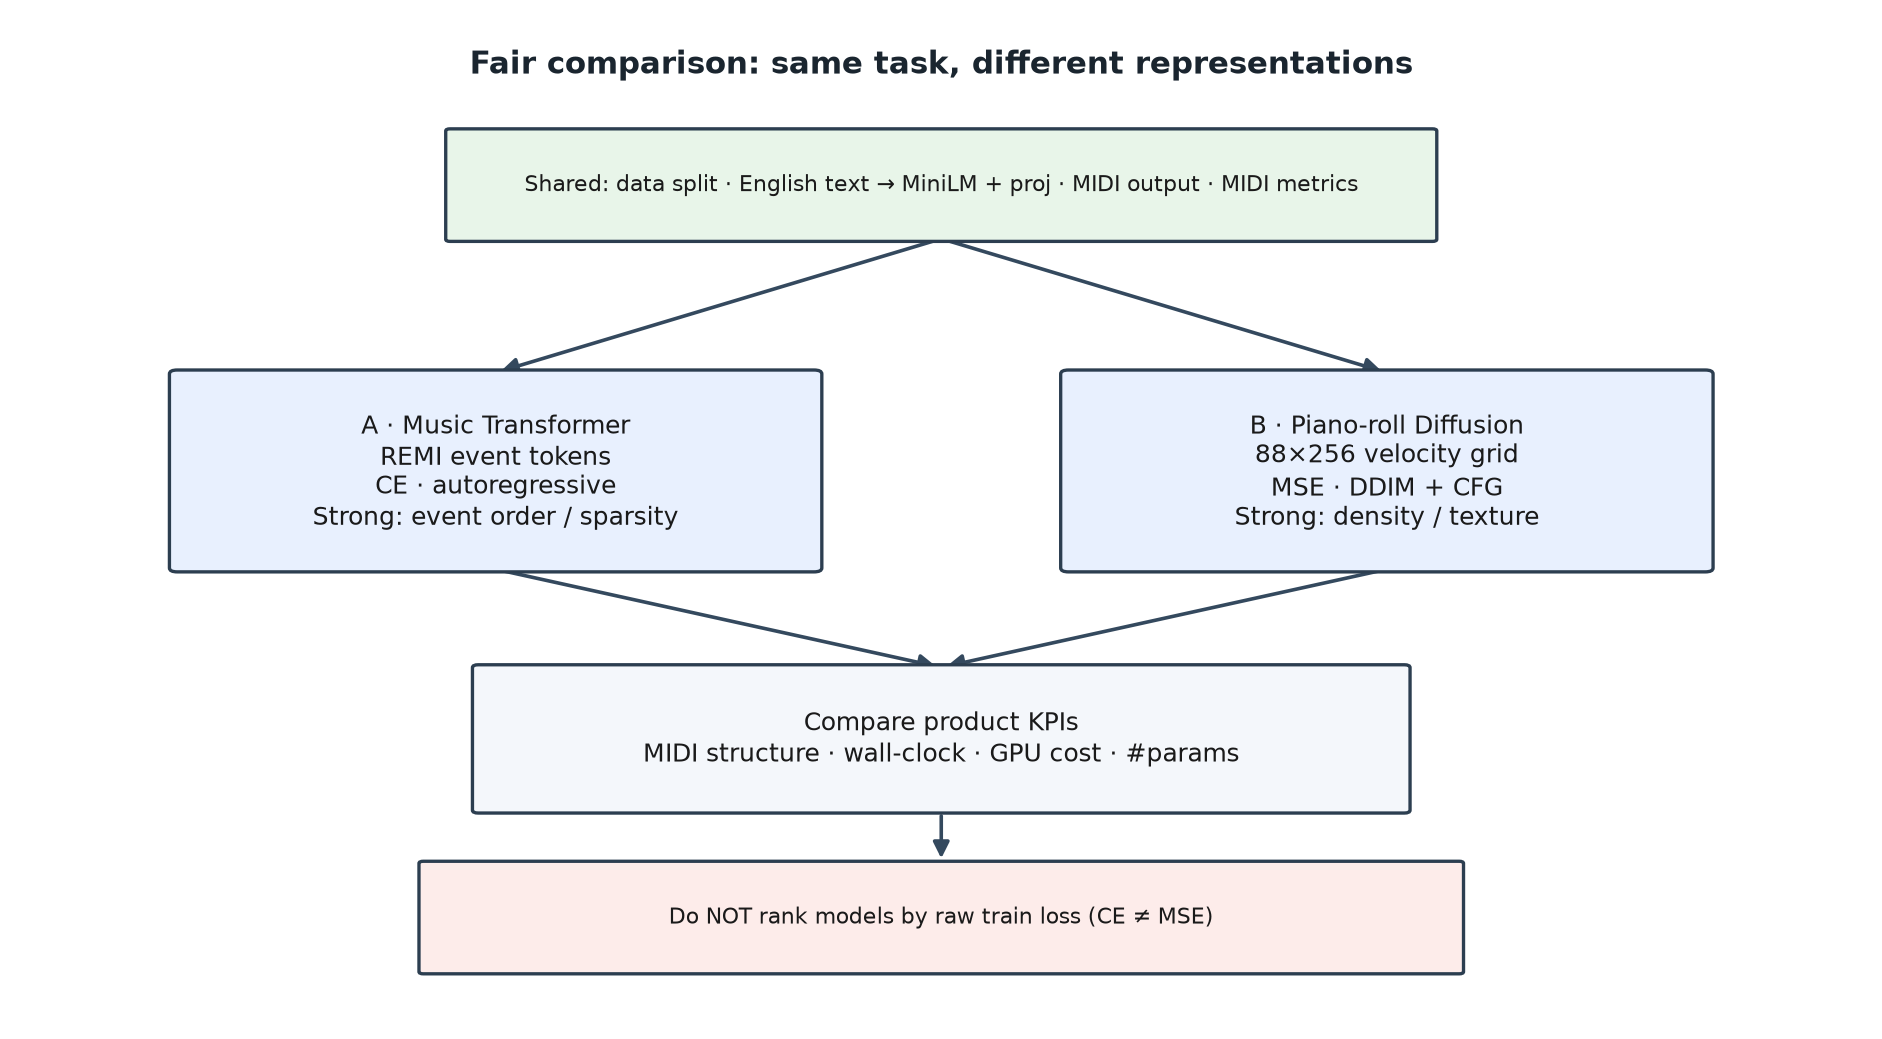
\includegraphics[width=0.92\textwidth]{he-qua}
    \caption{Hệ quả phương pháp: cùng dữ liệu, cùng pipeline text và đầu ra MIDI,
    nhưng khác biểu diễn/hàm mất mát --- chỉ so KPI trên MIDI và chi phí, không xếp hạng bằng CE hay MSE.}
    \label{fig:ch2-he-qua}
\end{figure}

\begin{figure}[htbp]
    \centering
    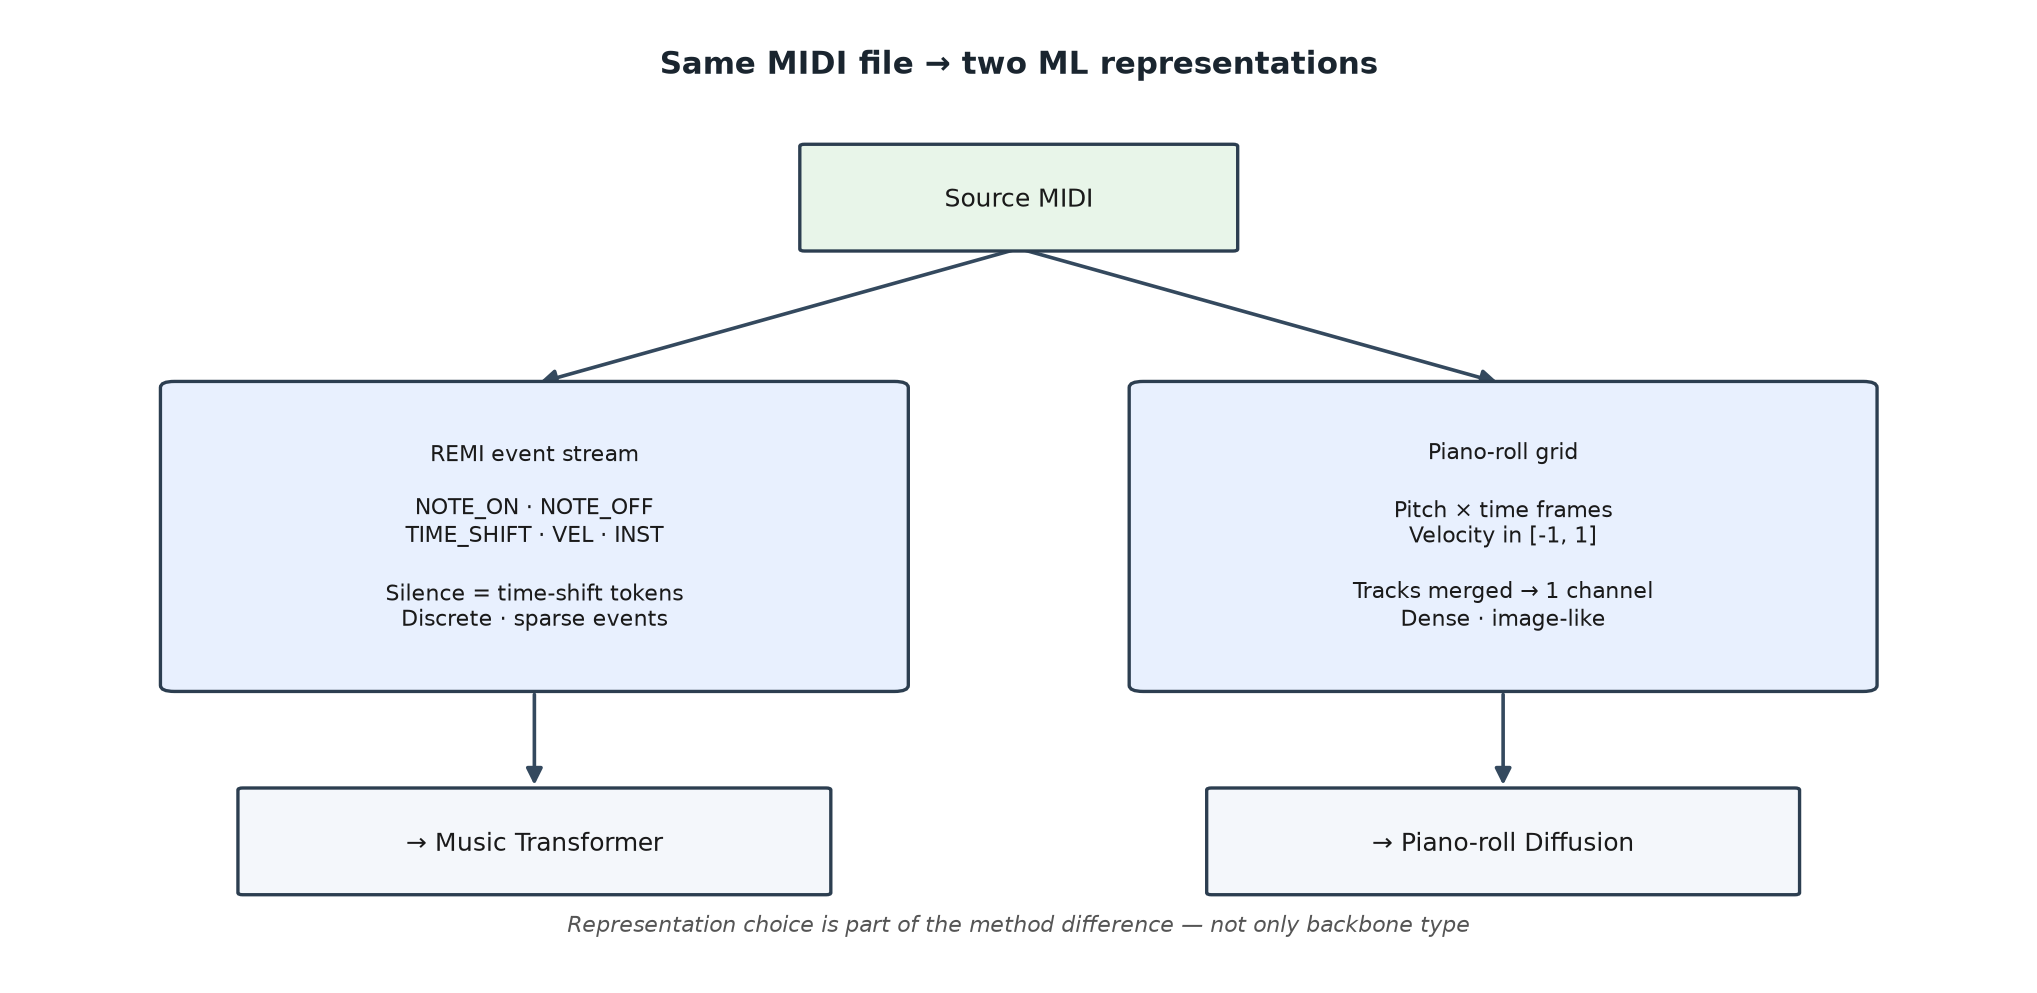
\includegraphics[width=0.92\textwidth]{fig_ch2_remi_vs_pianoroll}
    \caption{Cùng một tệp MIDI được mã hóa theo hai biểu diễn: chuỗi sự kiện REMI
    (nhánh Transformer) và lưới piano-roll một kênh (nhánh Diffusion).}
    \label{fig:ch2-remi-vs-roll}
\end{figure}

%------------------------------------------------------------------------------
\section{Mô hình tự hồi quy và Transformer trong sinh nhạc}
\label{sec:ch2-ar-transformer}

\subsection{Nguyên lý tự hồi quy}

Mô hình tự hồi quy (\textit{autoregressive}, AR) phân rã phân phối liên hợp theo xích quy tắc:

\begin{equation}
\label{eq:ar-factor}
p(y_{1:T}\mid c)
= \prod_{t=1}^{T}
p\!\left(y_t \mid y_{<t},\, c\right).
\end{equation}

Huấn luyện thường dùng teacher forcing: đưa $y_{<t}$ đúng từ dữ liệu, tối đa hóa log-likelihood (tương đương cực tiểu entropy chéo). Độ bối rối (\textit{perplexity}) $\exp(\mathcal{L})$ là thước đo khả năng dự đoán trung bình; độ bối rối giảm nghĩa là mô hình gán xác suất cao hơn cho token đúng trên tập đánh giá, nhưng không đồng nhất với chất lượng cảm nhận nghe.

\subsection{Transformer decoder}

Kiến trúc Transformer~\cite{vaswani2017attention} dùng self-attention để mô hình hóa phụ thuộc xa tốt hơn RNN, và huấn luyện song song theo chiều thời gian (với mask nhân quả khi là decoder ngôn ngữ). Với sinh nhạc, decoder-only (hoặc encoder--decoder) trên token MIDI đã được chứng minh trong các công trình như Music Transformer~\cite{huang2018music}, nhấn mạnh \textit{relative attention} để nắm các mẫu lặp theo khoảng cách tương đối --- phù hợp motif và nhịp.

Trong thực hành hiện đại, nhiều biến thể thay absolute position bằng RoPE, dùng GQA để giảm KV-cache, chuẩn hóa Q/K, và FFN kiểu SwiGLU. Các kỹ thuật này không đổi bản chất~\eqref{eq:ar-factor} nhưng cải thiện ổn định và chi phí suy luận --- đúng hướng các khối attention/layer trong nhánh Transformer của đồ án (chi tiết triển khai ở Chương~\ref{chap:implementation}).

\begin{figure}[htbp]
    \centering
    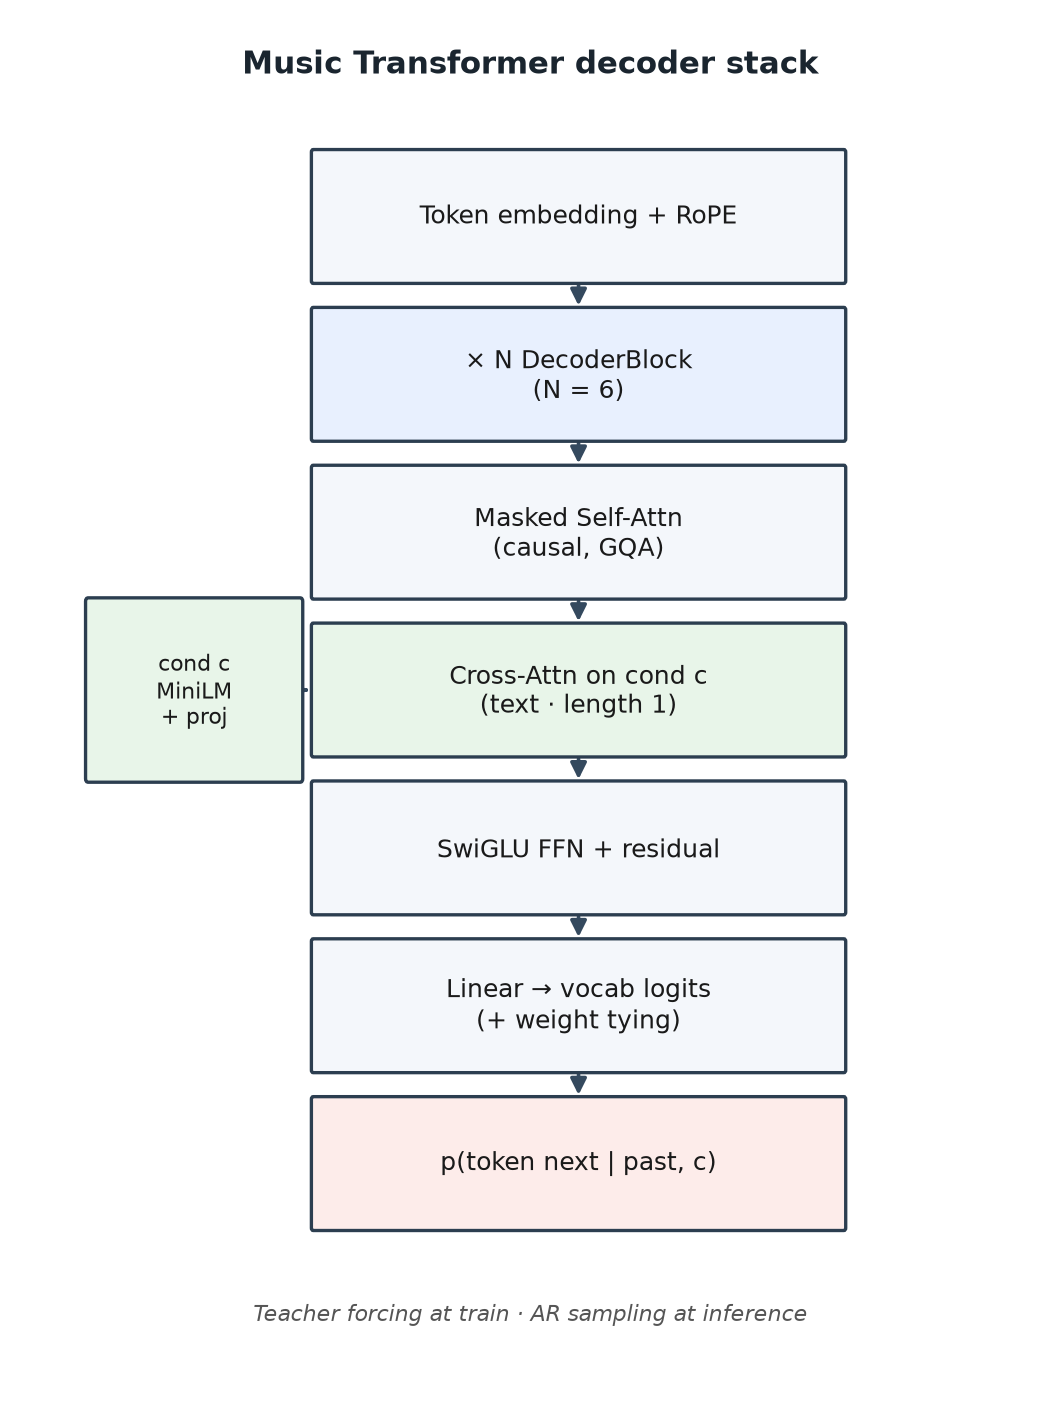
\includegraphics[width=0.55\textwidth]{Transformer_decoder}
    \caption{Ngăn xếp decoder của Music Transformer: embedding + RoPE, $N{=}6$
    DecoderBlock (self-attention nhân quả, cross-attention với $c$ text, FFN),
    đầu ra logits vocabulary.}
    \label{fig:ch2-transformer-decoder}
\end{figure}

\subsection{Điều kiện hóa trong Transformer}

Có nhiều cách đưa $c$ vào mô hình AR: nối prefix token, điều chế theo đặc trưng, hoặc \textbf{cross-attention} (query từ ẩn music, key/value từ biểu diễn điều kiện). Cross-attention cho phép mỗi vị trí chuỗi tham chiếu điều kiện ở mọi lớp, phù hợp khi $c$ là biểu diễn nhúng toàn cục hoặc chuỗi ngắn. Nếu $c$ chỉ gồm \textbf{một} vector (một ``token'' điều kiện), mô hình nhận thiên lệch điều kiện toàn cục lặp lại; khả năng nhấn mạnh từng thuộc tính (ví dụ chỉ instrument) bị hạn chế trừ khi tách điều kiện nhiều token hoặc bổ sung hàm mất mát phụ.

\begin{figure}[htbp]
    \centering
    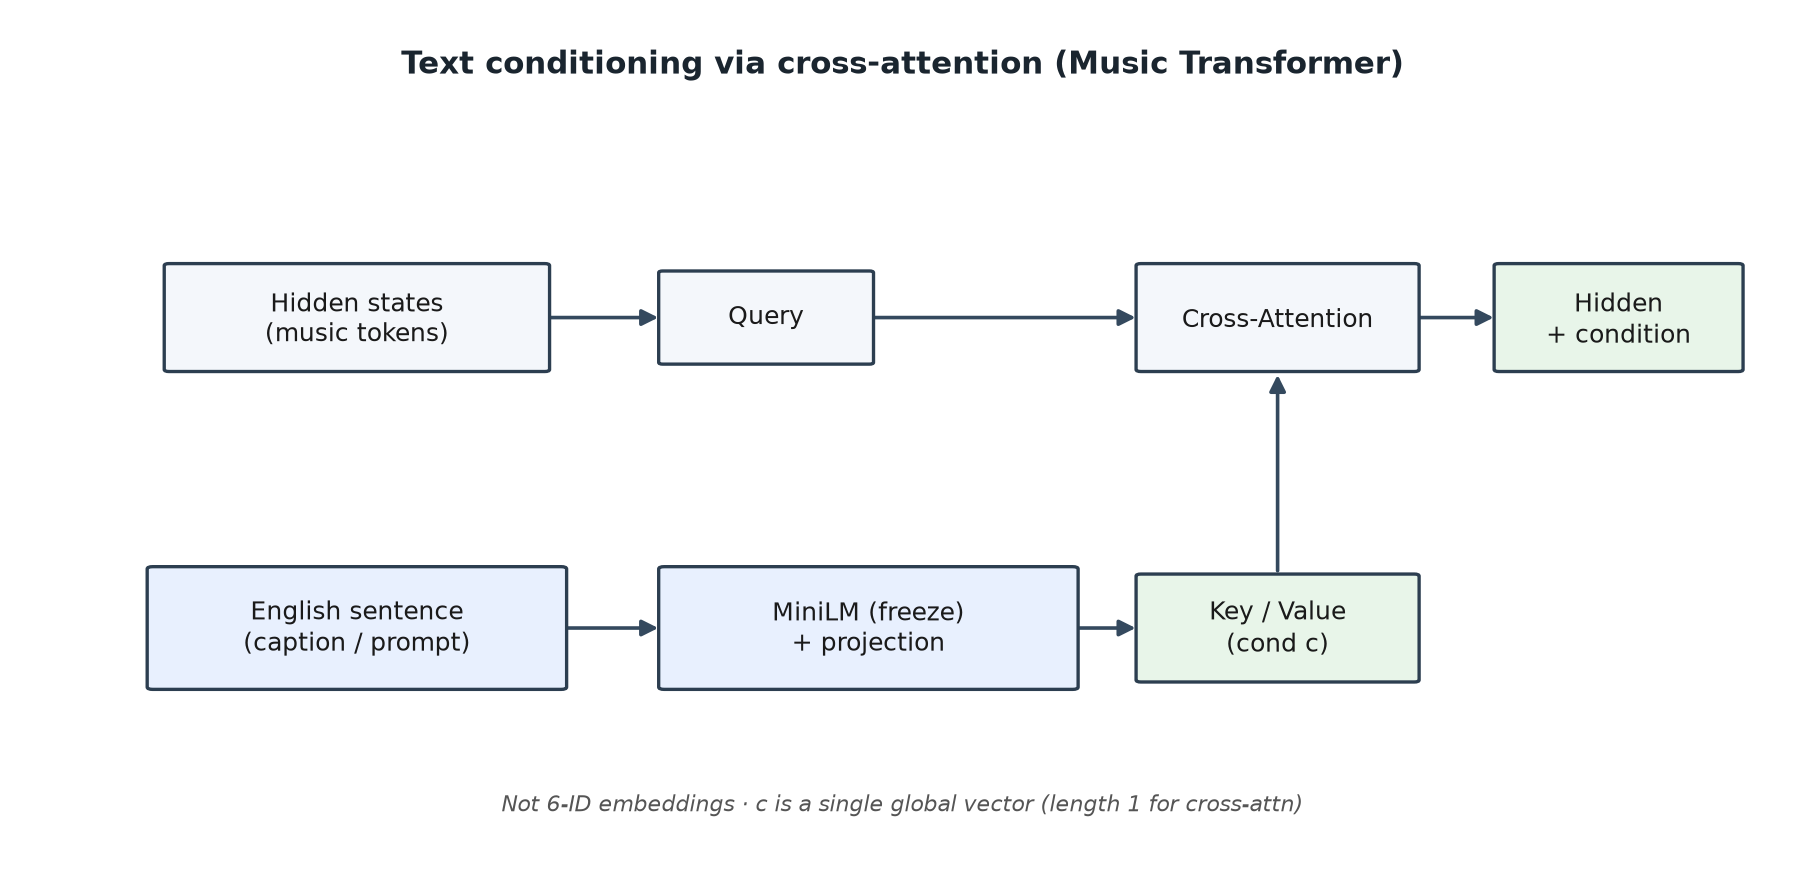
\includegraphics[width=0.95\textwidth]{dieu_Kien_hoa}
    \caption{Điều kiện hóa text trong Transformer: câu English $\rightarrow$ MiniLM
    đóng băng + projection $\rightarrow$ vector $c$ làm Key/Value cho cross-attention
    (không còn nhúng sáu ID).}
    \label{fig:ch2-conditioning}
\end{figure}

\subsection{Lấy mẫu chuỗi}

Tại suy luận, $y_t$ được lấy từ $p_\theta(\cdot\mid y_{<t},c)$ sau khi phân phối đã được làm sắc hoặc phẳng. Temperature $\tau$ chia logits: $\tau<1$ thiên về lựa chọn tham lam, $\tau>1$ tăng đa dạng. Top-$k$ chỉ giữ $k$ token xác suất cao nhất, trong khi nucleus sampling (top-$p$)~\cite{holtzman2020curious} giữ tập token nhỏ nhất có khối lượng xác suất không nhỏ hơn $p$. Với âm nhạc, kết hợp $\tau$ vừa phải và top-$p$ thường được ưa chuộng vì hạn chế token nhiễu ở đuôi phân phối mà vẫn không cứng nhắc như giải mã tham lam (\textit{greedy}). Điểm yếu cố hữu của AR vẫn là dừng sớm (\texttt{EOS}), lặp mẫu, hoặc lệch dần khỏi điều kiện khi chuỗi dài.
\begin{figure}[htbp]
    \centering
    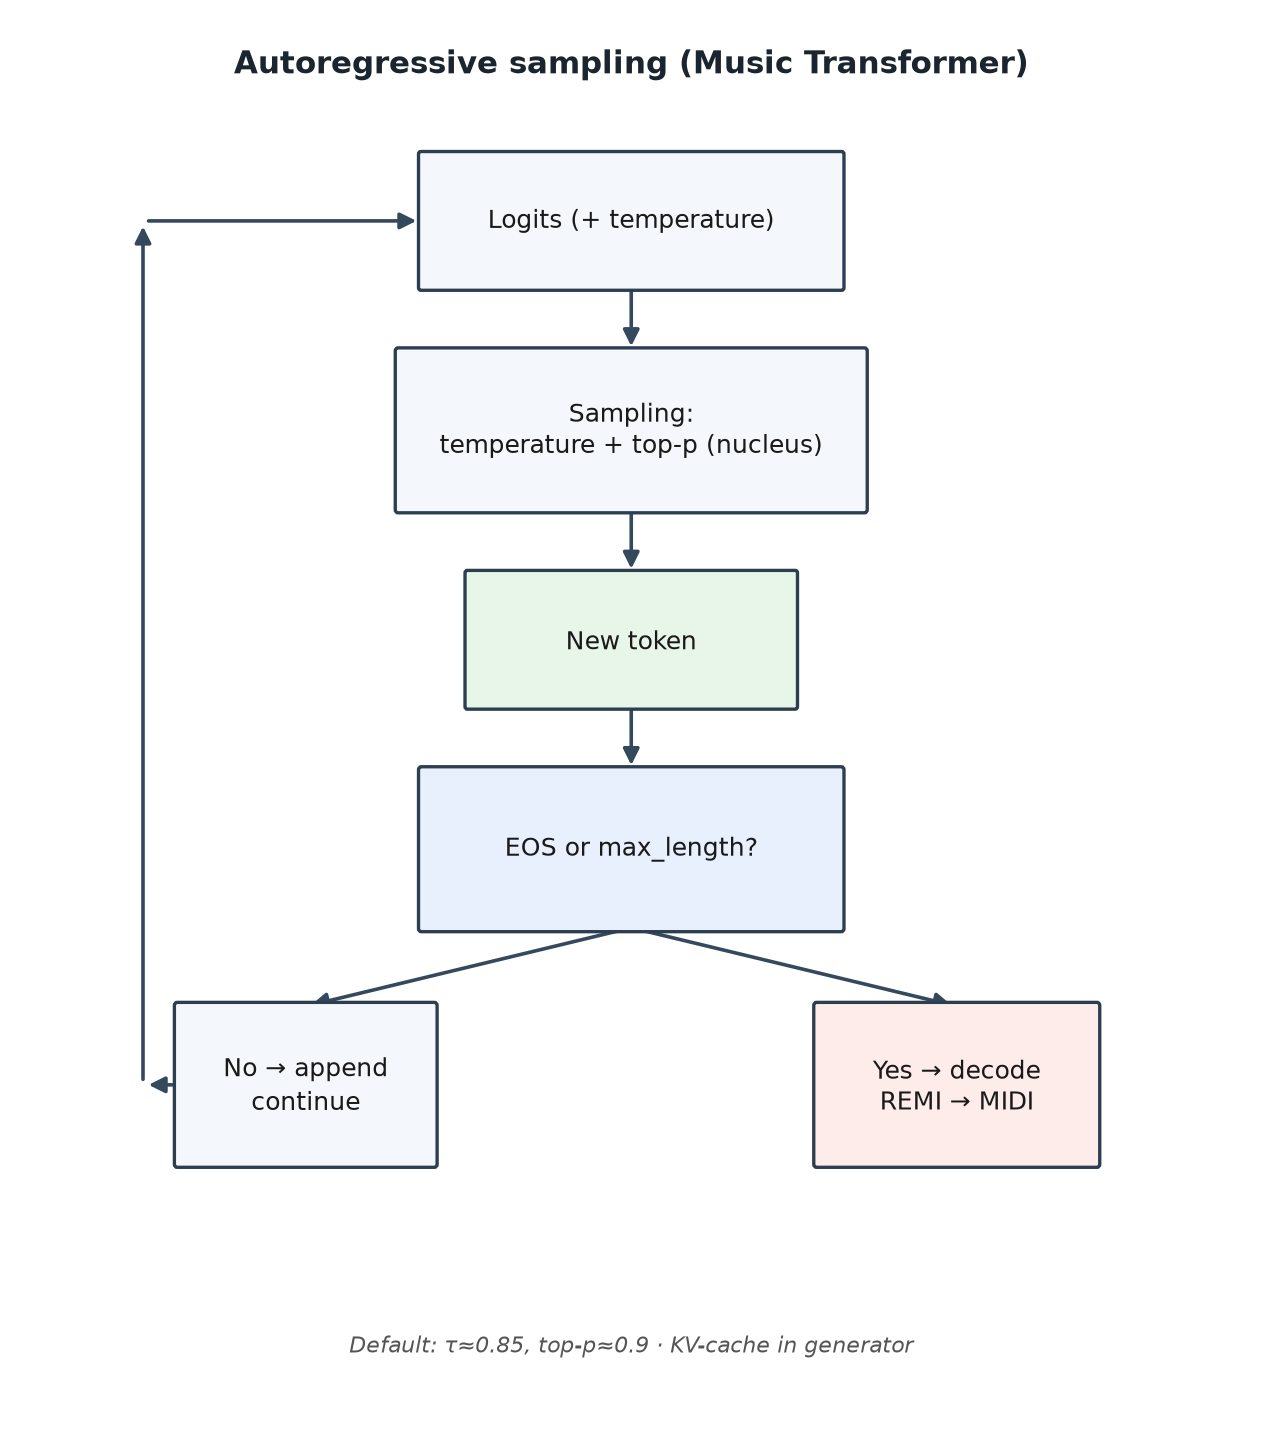
\includegraphics[width=0.55\textwidth]{lay_mau_chuoi}
    \caption{Lấy mẫu tự hồi quy tại suy luận: temperature + top-$p$, dừng khi
    \texttt{EOS}/độ dài tối đa, giải mã REMI $\rightarrow$ MIDI
    (mặc định $\tau{\approx}0{,}85$, top-$p{\approx}0{,}9$).}
    \label{fig:ch2-ar-sampling}
\end{figure}

%------------------------------------------------------------------------------
\section{Mô hình khuếch tán}
\label{sec:ch2-diffusion}

\subsection{Quy trình xuôi và ngược}

Mô hình khuếch tán khử nhiễu (\textit{denoising diffusion})~\cite{ho2020ddpm} định nghĩa quá trình Markov xuôi dần thêm nhiễu Gaussian vào dữ liệu $x_0$ cho tới gần $\mathcal{N}(0,I)$. Với lịch $\beta_t$ (hoặc tương đương $\alpha_t=1-\beta_t$, $\bar\alpha_t=\prod_{s=1}^t\alpha_s$), có dạng đóng:

\begin{equation}
\label{eq:ddpm-forward}
q(x_t\mid x_0)
= \mathcal{N}\!\left(
x_t;\,
\sqrt{\bar\alpha_t}\, x_0,\,
(1-\bar\alpha_t)I
\right).
\end{equation}

Mạng $\epsilon_\theta$ học dự đoán nhiễu $\epsilon$ đã trộn vào $x_t$ (hoặc học $x_0$/score tương đương). Hàm mất mát đơn giản phổ biến:

\begin{equation}
\label{eq:ddpm-loss}
\mathcal{L}_{\mathrm{simple}}
= \mathbb{E}_{x_0,t,\epsilon}
\big\|
\epsilon - \epsilon_\theta(x_t, t)
\big\|_2^2.
\end{equation}

Lịch \textbf{cosine} cho $\bar\alpha_t$~\cite{nichol2021improved} thường mượt hơn lịch linear ở nhiều tác vụ sinh, và được dùng trong cấu hình diffusion của đồ án.

\subsection{DDIM}

Denoising Diffusion Implicit Models~\cite{song2021ddim} cho phép lấy mẫu với ít bước hơn DDPM gốc, với tham số $\eta$ điều khiển mức ngẫu nhiên; $\eta=0$ cho quỹ đạo xác định. Điều này quan trọng khi UNet tốn kém về tính toán: thực nghiệm đồ án dùng hàng chục bước DDIM (cỡ 80) thay vì đủ 1000 bước đầy đủ mỗi lần sinh.
\begin{figure}[htbp]
    \centering
    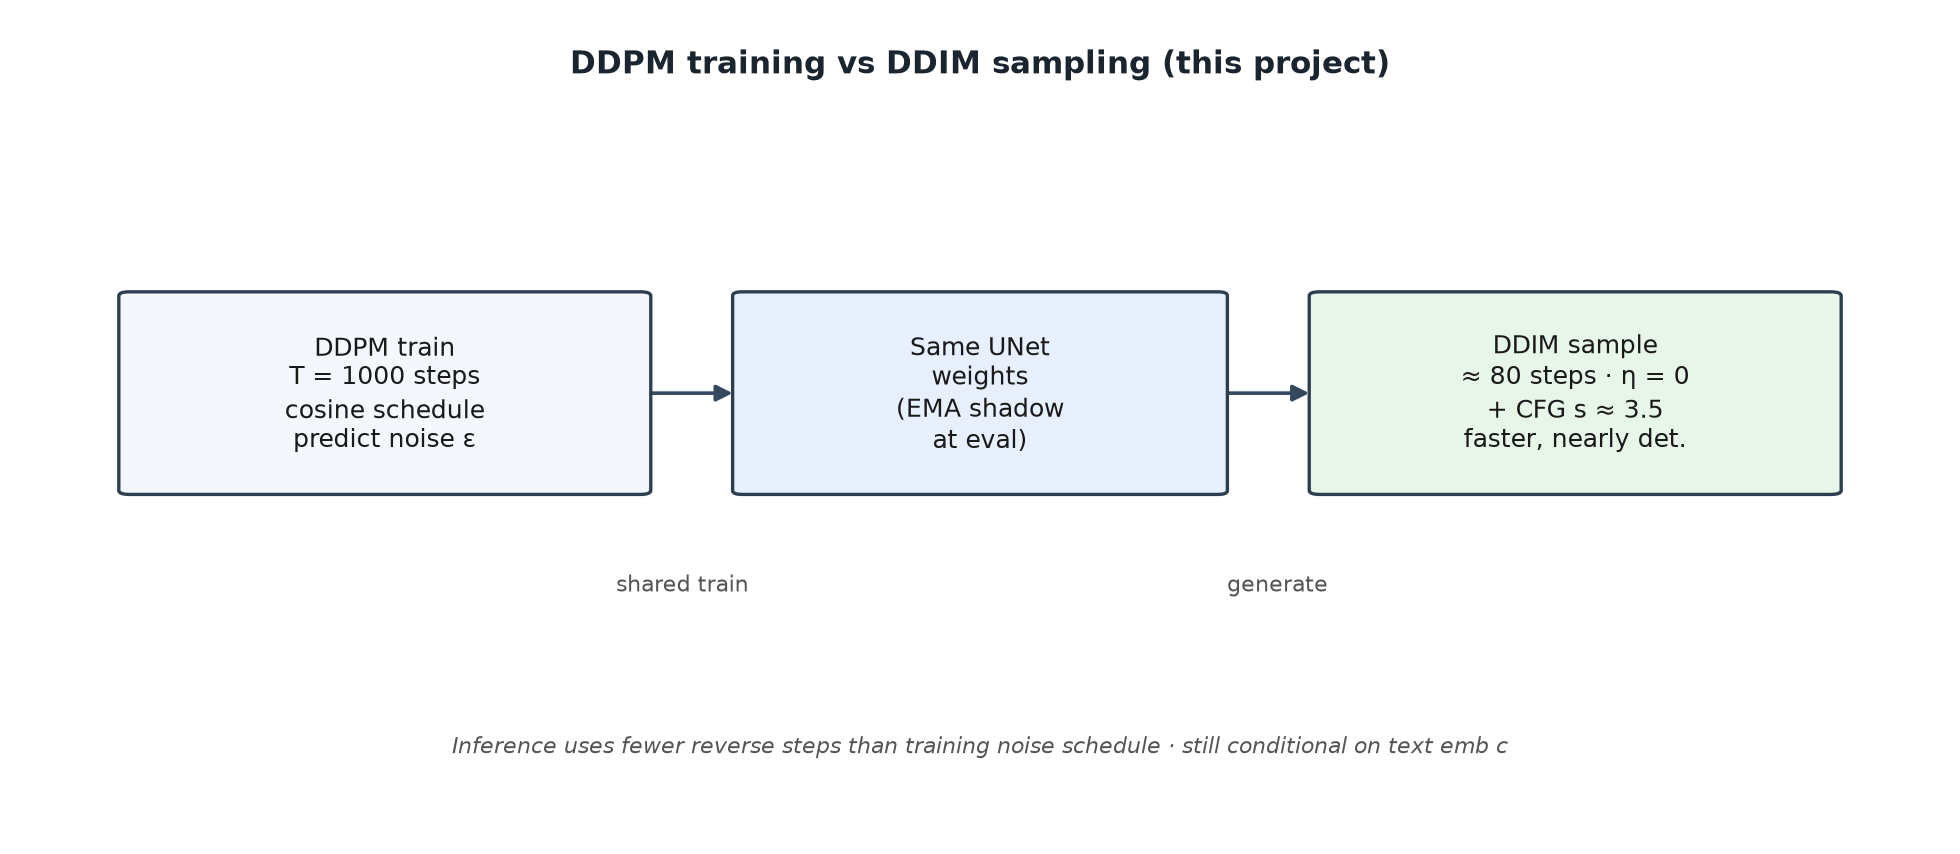
\includegraphics[width=0.95\textwidth]{ddim}
    \caption{Huấn luyện theo lịch DDPM ($T{=}1000$, cosine) và lấy mẫu DDIM
    (khoảng 80 bước, $\eta{=}0$) trên cùng UNet, kèm CFG khi generate.}
    \label{fig:ch2-ddim}
\end{figure}

\subsection{Điều kiện hóa và classifier-free guidance}

Với $c$ cho trước, mô hình học $\epsilon_\theta(x_t,t,c)$. \textbf{Classifier-free guidance} (CFG)~\cite{ho2022cfg} huấn luyện xen kẽ (hoặc ngẫu nhiên loại bỏ) điều kiện rỗng $\emptyset$, rồi khi lấy mẫu:


\begin{figure}[htbp]
    \centering
    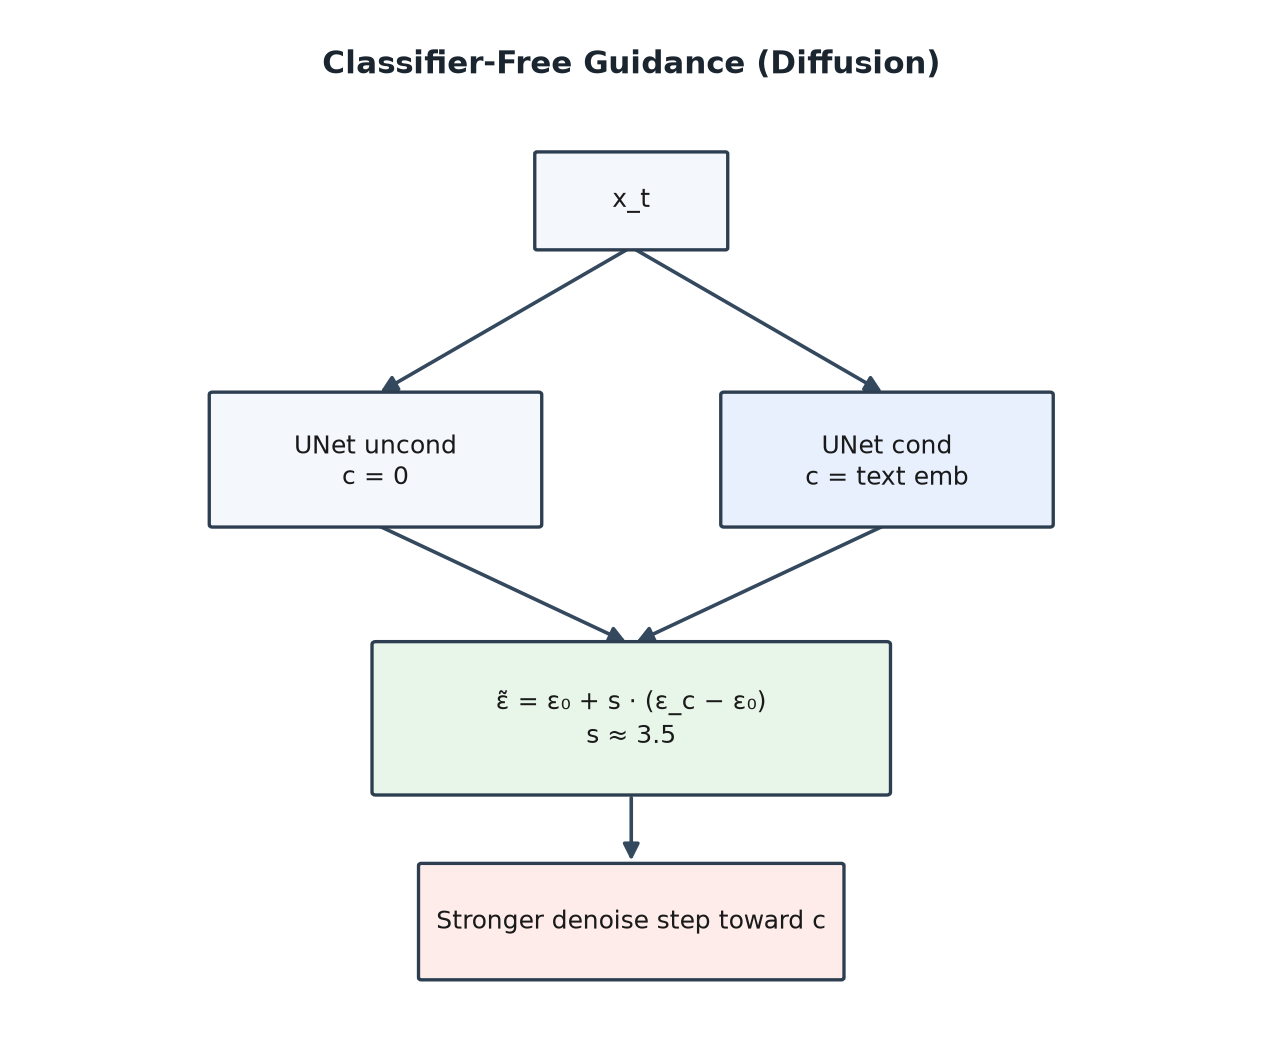
\includegraphics[width=0.72\textwidth]{classifierfree_guidance}
    \caption{Classifier-free guidance: kết hợp dự đoán có/không điều kiện text
    với hệ số $s{\approx}3{,}5$ (điều kiện rỗng là vector $\mathbf{0}$).}
    \label{fig:ch2-cfg}
\end{figure}

\begin{equation}
\label{eq:cfg-theory}
\tilde\epsilon
= \epsilon_\theta(x_t,t,\emptyset)
+ s\cdot\bigl(
\epsilon_\theta(x_t,t,c)
-
\epsilon_\theta(x_t,t,\emptyset)
\bigr).
\end{equation}

Hệ số $s>1$ tăng độ bám $c$, nhưng có thể làm mẫu cứng nhắc hoặc làm tăng biên độ kích hoạt --- trên piano-roll có thể ảnh hưởng mật độ kích hoạt sau giải mã. FiLM/feature-wise modulation là một cách tiết kiệm để đưa $c$ (và biểu diễn nhúng thời gian $t$) vào ResBlock CNN, thay cho cross-attention dày trên mọi vị trí không gian.

\subsection{EMA}

Trung bình trượt tham số (\textit{exponential moving average}) thường dùng khi lấy mẫu diffusion để ổn định. Đồ án áp EMA cho UNet và prompt encoder khi kiểm định/sinh --- chi tiết ở Chương~\ref{chap:implementation}.

\subsection{Giới hạn khi áp dụng cho piano-roll MIDI}

Hàm mất mát~\eqref{eq:ddpm-loss} tối ưu khử nhiễu trên không gian liên tục đã chọn. Nó \textbf{không} trực tiếp tối ưu số nốt, tính thưa, hay đúng chương trình nhạc cụ MIDI. Mọi ánh xạ roll $\rightarrow$ MIDI (ngưỡng, thời lượng tối thiểu, gán program) nằm ngoài gradient. Do đó MSE kiểm định thấp là điều kiện cần cho bộ khử nhiễu tốt, chưa đủ để kết luận BGM đạt chất lượng nghe mong muốn hay mật độ hợp lý --- luận điểm sẽ được kiểm chứng bằng các chỉ số MIDI ở Chương~\ref{chap:experiments}.

\begin{figure}[htbp]
    \centering
    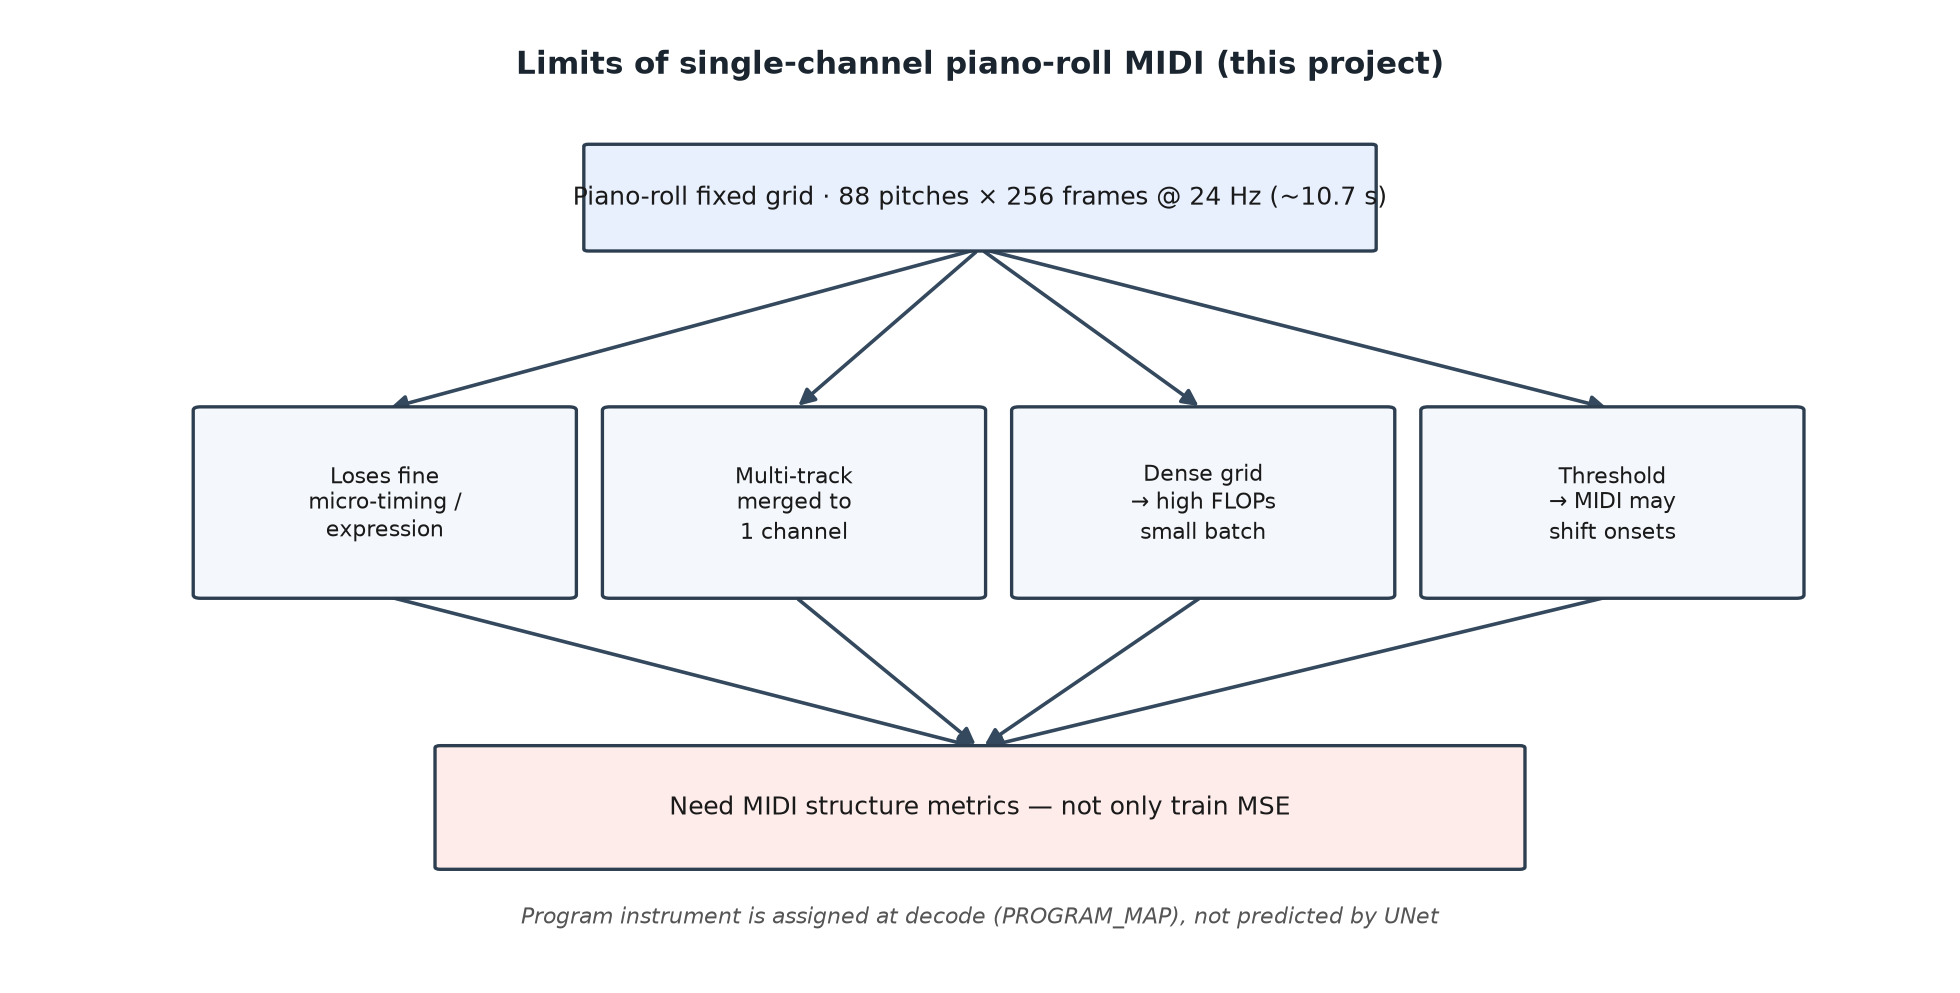
\includegraphics[width=0.92\textwidth]{gioihanpiano-roll-MIDI}
    \caption{Hạn chế piano-roll một kênh trong đồ án: mất micro-timing, gộp track,
    lưới dày tốn FLOPs, và giải mã ngưỡng có thể lệch onset --- cần metric MIDI
    ngoài MSE train; program nhạc cụ gán sau sinh.}
    \label{fig:ch2-pianoroll-limits}
\end{figure}

\begin{figure}[htbp]
    \centering
    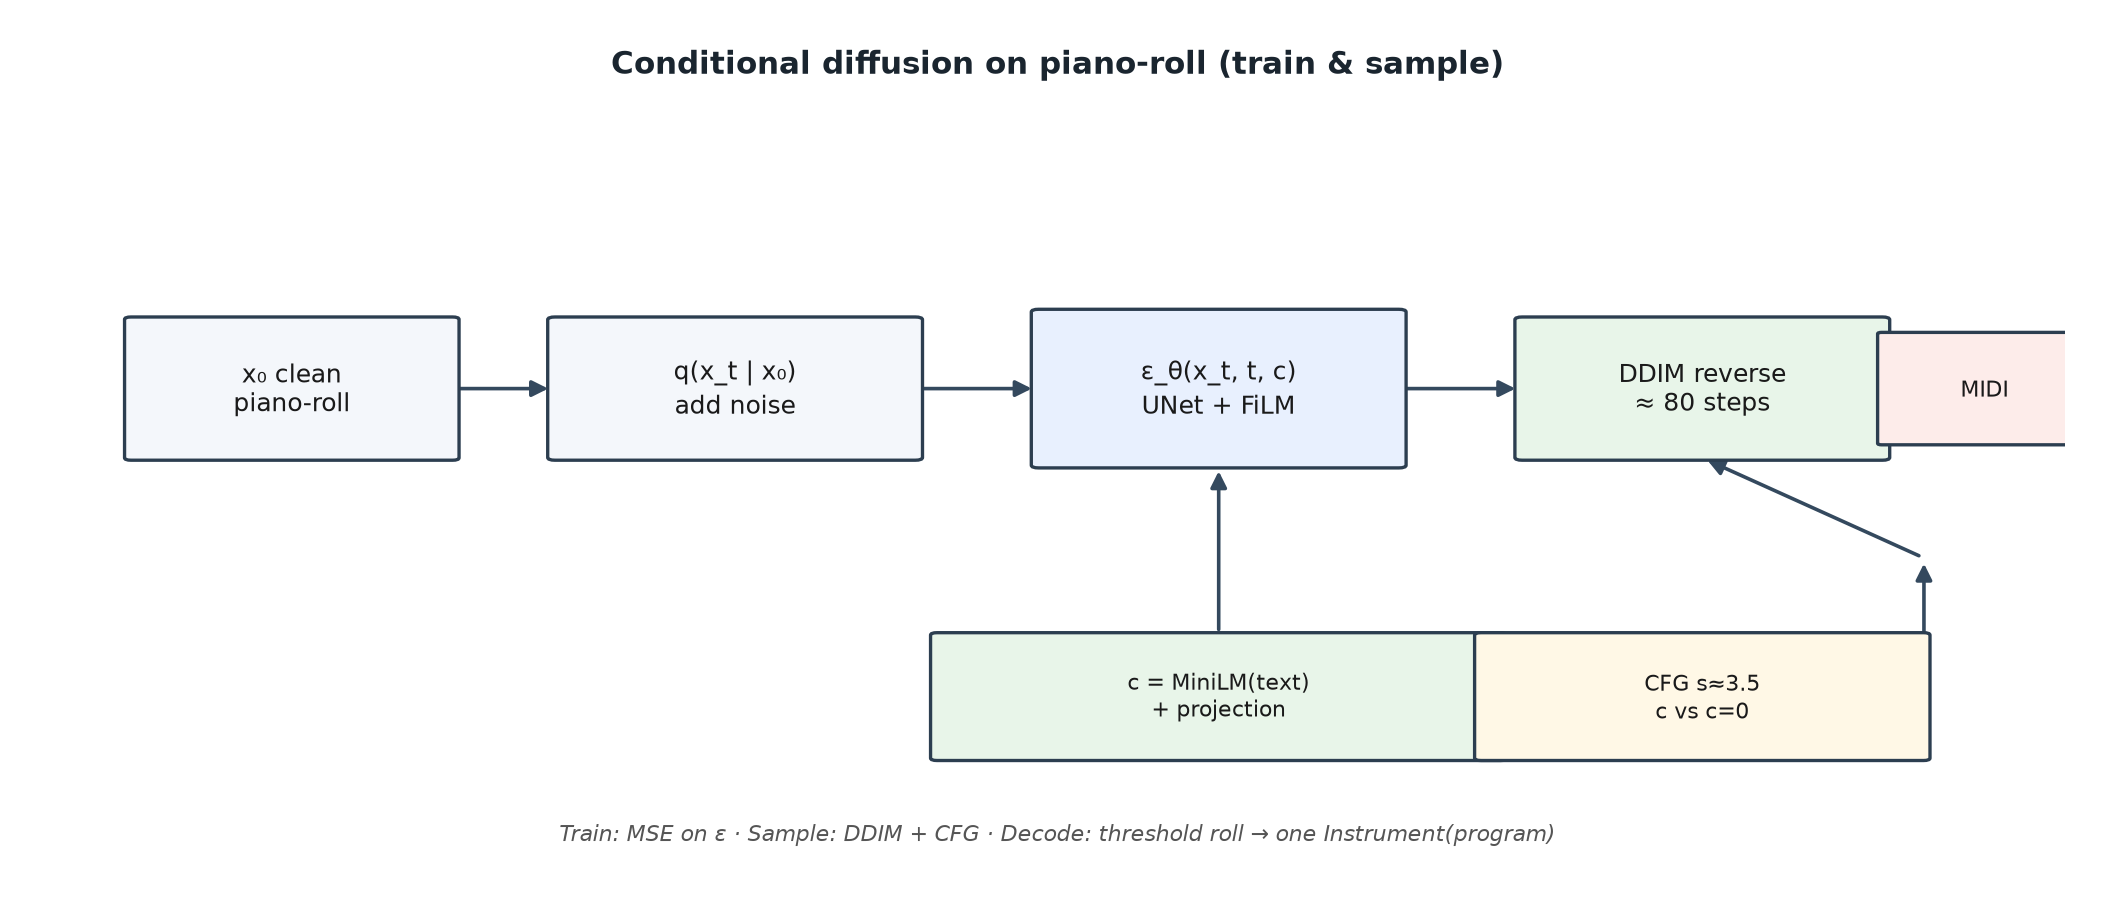
\includegraphics[width=0.95\textwidth]{fig_ch2_diffusion_process}
    \caption{Quy trình diffusion có điều kiện trên piano-roll: thêm nhiễu từ $x_0$,
    UNet dự đoán $\epsilon$ với $c$ (MiniLM+proj) qua FiLM, lấy mẫu DDIM + CFG,
    rồi giải mã sang MIDI.}
    \label{fig:ch2-diffusion-process}
\end{figure}


%------------------------------------------------------------------------------
\section{Công trình liên quan}
\label{sec:ch2-related}

\subsection{Sinh MIDI bằng mô hình chuỗi}

Music Transformer~\cite{huang2018music} cho thấy self-attention (đặc biệt relative) sinh được cấu trúc dài hạn trên piano MIDI. Các hệ lớn hơn theo hướng GPT/Sparse Transformer (ví dụ các mô tả công khai quanh MuseNet) mở rộng đa nhạc cụ và phong cách, nhưng quy mô và chi tiết toàn hệ thống thường vượt khuôn khổ project. Điểm chung: AR kết hợp token sự kiện là đường cơ sở vững cho MIDI.

\begin{figure}[htbp]
    \centering
    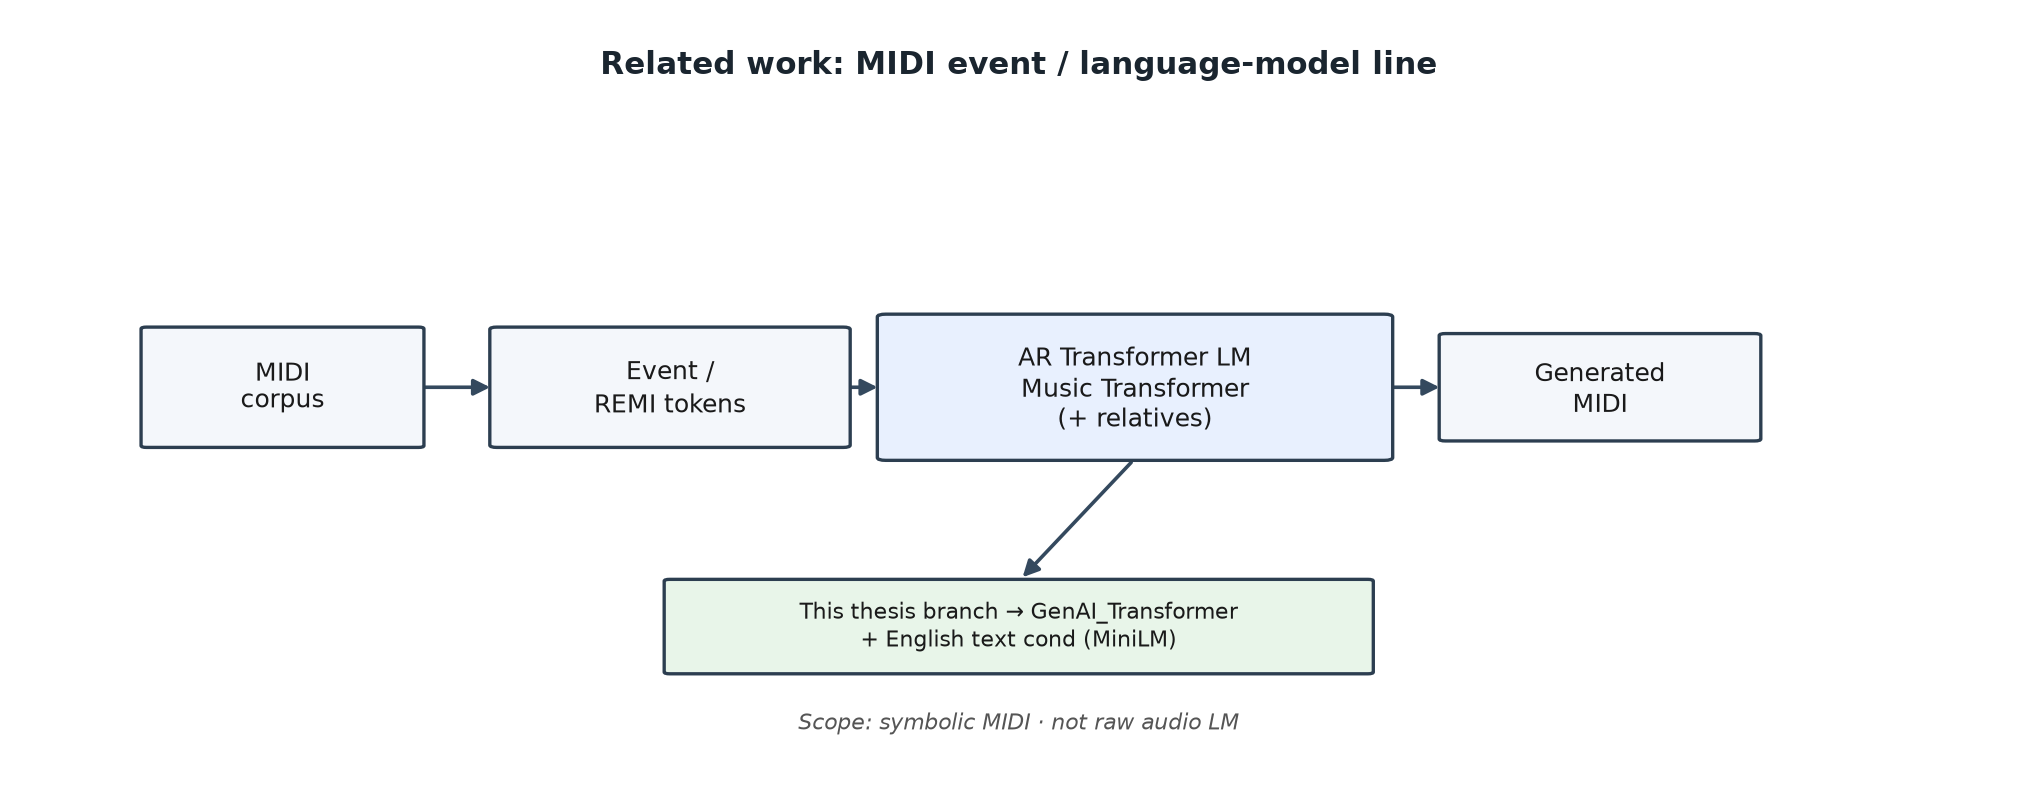
\includegraphics[width=0.95\textwidth]{sinhMiDIbangongtrinhchuoi}
    \caption{Dòng nghiên cứu sinh MIDI bằng mô hình ngôn ngữ / Transformer trên
    token sự kiện; nhánh đồ án là \texttt{GenAI\_Transformer} có điều kiện text (MiniLM).}
    \label{fig:ch2-related-midi-seq}
\end{figure}

\subsection{Sinh audio từ văn bản}

MusicLM~\cite{agostinelli2023musiclm} kết hợp embedding nhạc--ngôn ngữ và sinh token audio đa cấp. MusicGen~\cite{copet2023musicgen} đơn giản hóa còn single-stage language model trên token audio nén. Các hệ này đặt chuẩn chất lượng nghe và text free-form, đồng thời cho thấy chi phí dữ liệu/tính toán rất cao. Project \textbf{không} tái hiện các hệ này; chúng là mốc tham chiếu về khả năng text-to-music audio ở quy mô lớn.

\begin{figure}[htbp]
    \centering
    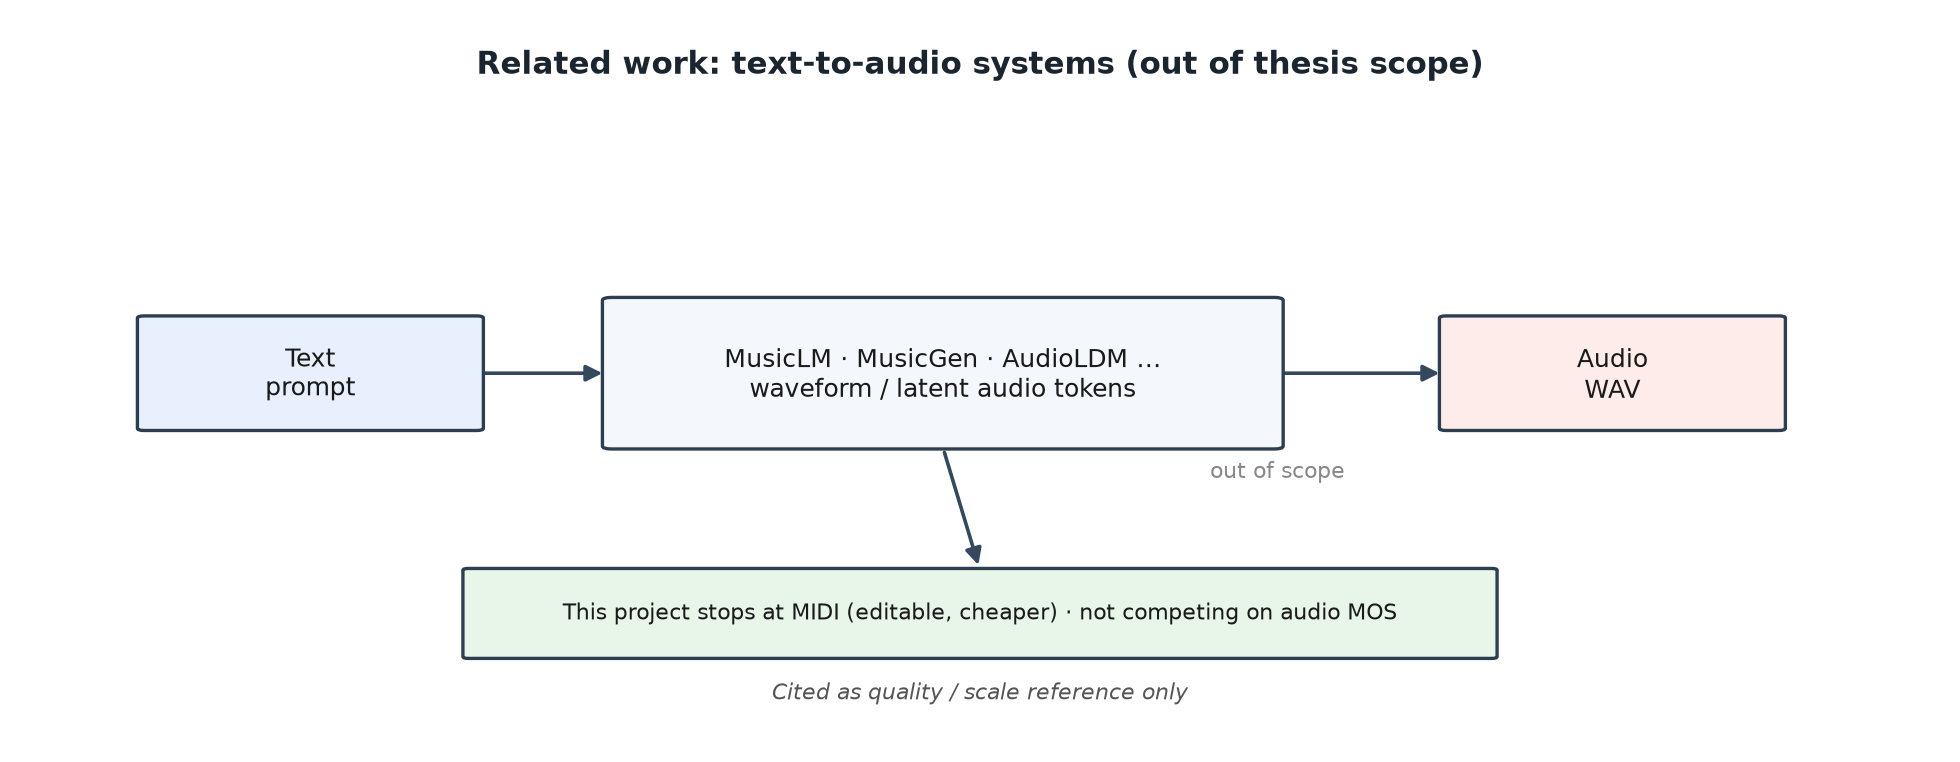
\includegraphics[width=0.92\textwidth]{audio-tu-van-ban}
    \caption{Các hệ text-to-audio quy mô lớn (MusicLM, MusicGen, AudioLDM, \ldots)
    nằm ngoài phạm vi đồ án; báo cáo chỉ dùng làm mốc tham chiếu về chất lượng/scale.}
    \label{fig:ch2-related-text-audio}
\end{figure}

\subsection{Diffusion cho âm thanh và biểu diễn 2D}

AudioLDM và các biến thể latent diffusion trên mel-spectrogram~\cite{liu2023audioldm} minh họa sức mạnh diffusion khi có autoencoder và điều kiện hóa mạnh. Trên MIDI, diffusion trực tiếp trên piano-roll là đơn giản hóa mang tính giáo dục/so sánh: không VAE latent, không CLAP, dễ triển khai nhưng chịu hạn chế biểu diễn gộp track đã bàn.


\begin{figure}[htbp]
    \centering
    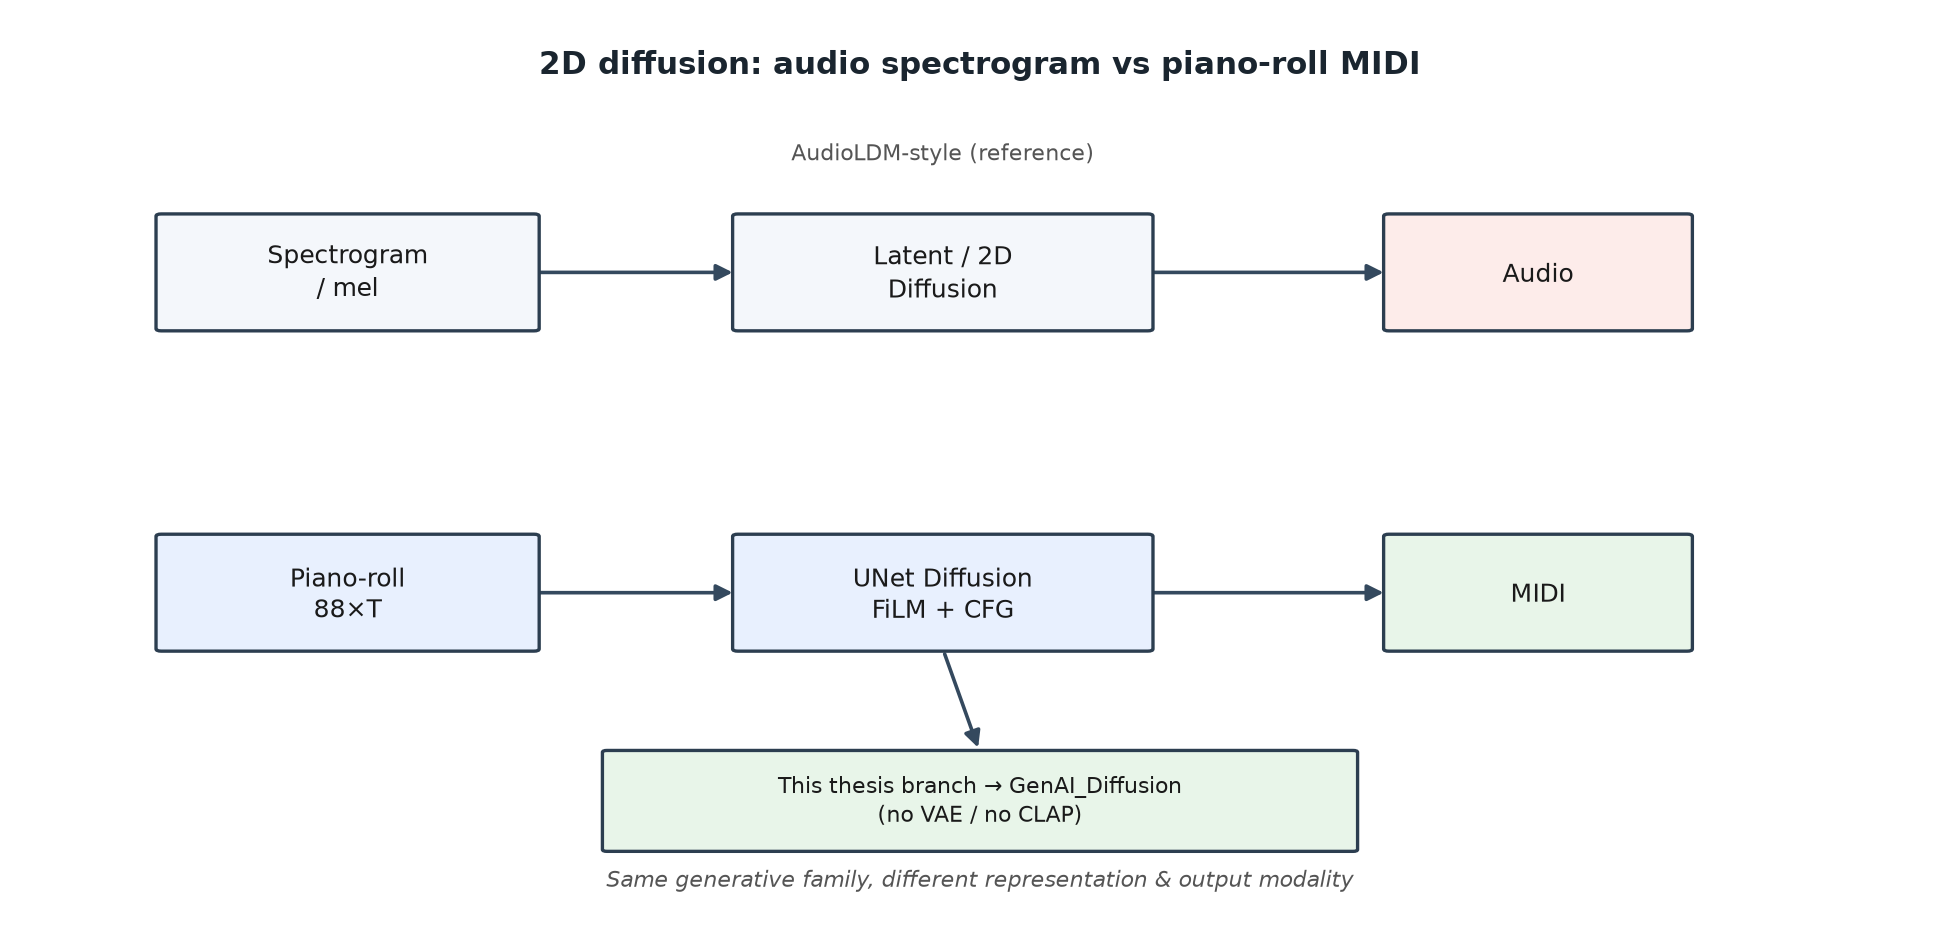
\includegraphics[width=0.92\textwidth]{diffusion-2d}
    \caption{Hai nhánh diffusion 2D: spectrogram/latent audio (tham chiếu) so với
    piano-roll $\rightarrow$ MIDI của nhánh \texttt{GenAI\_Diffusion} (không VAE/CLAP).}
    \label{fig:ch2-related-diff2d}
\end{figure}

\subsection{Dữ liệu có thuộc tính cho nhạc}

ComMU~\cite{commu2023} cung cấp MIDI kèm siêu dữ liệu có cấu trúc (thể loại, mood, \ldots), phù hợp học có điều kiện theo thuộc tính --- lý do ComMU chiếm tỉ trọng lớn trong kho gộp của đồ án. Các kho piano lớn như MAESTRO~\cite{hawthorne2018maestro} giàu chất lượng biểu diễn nhưng thiên solo piano và không luôn có nhãn game/mood đồng nhất.

\subsection{Vị trí báo cáo}

Bảng~\ref{tab:ch2-position} tóm tắt chỗ đứng phương pháp.

\begin{table}[htbp]
\centering
\caption{Đặt báo cáo trong bối cảnh nghiên cứu (mang tính định tính)}
\label{tab:ch2-position}
\small
\begin{tabular}{p{3.4cm}p{4.8cm}p{5.0cm}}
\toprule
\textbf{Hướng} & \textbf{Đặc trưng} & \textbf{Khác báo cáo này} \\
\midrule
Music Transformer gốc &
AR + relative attn, MIDI piano &
Thêm điều kiện text (MiniLM); so với diffusion; kỹ thuật thực dụng (GQA/RoPE) \\
\midrule
MusicLM / MusicGen &
Text $\rightarrow$ audio, scale lớn &
Báo cáo: MIDI, text nhẹ (MiniLM freeze), một GPU, so hai mô hình nền \\
\midrule
Audio LDM-style &
Latent diffusion audio &
Báo cáo: diffusion trên piano-roll trực tiếp, MiniLM chứ không CLAP/VAE \\
\midrule
Báo cáo này &
Cùng data + split + text encoder; REMI vs roll; chỉ số MIDI + chi phí &
Không khẳng định chất lượng nghe tiên tiến nhất; nhấn giao thức và diễn giải đúng chỉ số \\
\bottomrule
\end{tabular}
\end{table}

%------------------------------------------------------------------------------
\section{Tiêu chí so sánh hợp lệ giữa hai họ}
\label{sec:ch2-compare-criteria}

Từ các mục trên có thể rút vài nguyên tắc sẽ chi phối Chương~\ref{chap:implementation}--\ref{chap:experiments}. Trước hết, không so sánh trực tiếp entropy chéo và MSE vì khác không gian và đơn vị. Giao thức phải đồng nhất: cùng tệp MIDI huấn luyện/kiểm định, cùng lược đồ $c$, cùng prompt đánh giá, cùng họ chỉ số trên MIDI sinh. Khi đọc mật độ hay đa âm, cần tách phần đến từ biểu diễn và giải mã khỏi phần đến từ số layer hay optimizer. Chỉ số khớp instrument chỉ có nghĩa khi program thực sự do mô hình quyết định; nếu program bị gán cố định sau sinh, chỉ số không còn đo điều kiện hóa. Thời gian huấn luyện/suy luận cùng dung lượng tham số/VRAM là một phần của quyết định kỹ thuật, không phải phụ lục. Cuối cùng, nếu chưa có MOS hay thử nghiệm nghe, kết luận phải dừng ở cấu trúc sự kiện và hành vi học.

Các nguyên tắc này tạo cầu nối sang chương triển khai, nơi hai thiên kiến quy nạp được hiện thực hóa thành mã nguồn cụ thể.

%------------------------------------------------------------------------------
\section{Đánh giá sinh nhạc: từ likelihood đến chỉ số cấu trúc}
\label{sec:ch2-eval-theory}

Việc chọn thước đo quyết định cách diễn giải ``mô hình nào tốt hơn''. Có thể phân lớp thô như sau.

\paragraph{Likelihood / reconstruction.}
Entropy chéo và độ bối rối đo khả năng nén/dự đoán token; MSE diffusion đo sai số nhiễu. Chúng hữu ích để theo dõi hội tụ và so các lần chạy \textit{cùng} hàm mục tiêu, nhưng \textbf{không} chuyển đổi được giữa hai họ.

\paragraph{Chỉ số cấu trúc trên MIDI.}
Các đại lượng như mật độ nốt (số nốt trên một đơn vị thời gian), đa âm trung bình, tỉ lệ im lặng, entropy cao độ, khoảng cách histogram pitch-class tới tập tham chiếu cho phép so sánh tệp sinh mà không cần nghe. Ưu điểm: tự động, tái lập. Nhược: không nắm đường nét giai điệu dài hạn, cảm xúc chủ quan, hay mức phù hợp scene theo người nghe.

\paragraph{Chỉ số bám điều kiện.}
Đo xem đầu ra có phản ánh $c$ không. Ví dụ khớp nhóm nhạc cụ giữa prompt và program trội trong tệp. Chỉ số này chỉ hợp lệ khi program (hoặc proxy) thực sự phụ thuộc mô hình; nếu quy trình gán program từ nhãn sau khi sinh, điểm số không còn là thước đo tạo sinh.

\paragraph{Đánh giá người và chỉ số audio.}
MOS, thử nghiệm ưa thích, FAD, CLAP score gần chất lượng cảm nhận hơn nhưng tốn kém và, với MIDI, còn phụ thuộc synthesizer. Đồ án ghi nhận các hướng này như chuẩn mực cộng đồng, đồng thời khoanh phạm vi vào chỉ số cấu trúc kết hợp chi phí --- nhất quán với tài nguyên và mục tiêu phương pháp luận.

%------------------------------------------------------------------------------
\section{Kỳ vọng hành vi trước khi thực nghiệm}
\label{sec:ch2-bias-summary}

Trước khi chuyển sang mã nguồn, bảng~\ref{tab:ch2-bias} tóm tắt kỳ vọng hành vi suy ra từ lý thuyết --- các kỳ vọng này sẽ được \textbf{kiểm chứng hoặc bác bỏ một phần} bằng số liệu ở Chương~\ref{chap:experiments}.

\begin{table}[htbp]
\centering
\caption{Thiên kiến quy nạp và hệ quả kỳ vọng}
\label{tab:ch2-bias}
\small
\begin{tabular}{p{3.2cm}p{5.4cm}p{5.4cm}}
\toprule
\textbf{Yếu tố} & \textbf{AR + REMI} & \textbf{Diffusion + roll} \\
\midrule
Không gian quyết định &
Rời rạc, từng sự kiện &
Liên tục, từng ô lưới \\
\midrule
Im lặng &
Time-shift / không note &
Ô gần giá trị ``tắt''; dễ lệch nếu giải mã yếu \\
\midrule
Đa âm &
Phụ thuộc số NOTE\_ON chồng thời gian &
Phụ thuộc bao nhiêu pitch vượt ngưỡng cùng frame \\
\midrule
Instrument &
Token trong chuỗi &
Dễ mất nếu roll gộp; hoặc gán ngoài model \\
\midrule
Lỗi suy luận &
Tích lũy theo bước; EOS sớm &
Lệch toàn cục trên roll; nhạy threshold \\
\bottomrule
\end{tabular}
\end{table}

%------------------------------------------------------------------------------
\section*{Tóm tắt chương}
\addcontentsline{toc}{section}{Tóm tắt chương}

Chương~\ref{chap:theory} đã làm rõ bài toán sinh nhạc có điều kiện, đối lập biểu diễn chuỗi sự kiện và piano-roll, trình bày nền AR/Transformer kèm lấy mẫu, nền diffusion/DDIM/CFG, và khảo sát công trình liên quan để định vị đồ án như một nghiên cứu so sánh ở quy mô đồ án tốt nghiệp trên MIDI có điều kiện text (kèm nhãn cấu trúc). Chương tiếp theo mô tả chi tiết cách hai hướng được triển khai trên cùng đặc tả bài toán, đặc biệt pipeline mã hóa câu tiếng Anh (MiniLM đóng băng + projection).

\chapter{Triển khai hệ thống}
\label{chap:implementation}

Nếu Chương~\ref{chap:theory} trả lời câu hỏi \textit{vì sao hai họ tạo sinh khác nhau về bản chất}, chương này trả lời câu hỏi cụ thể hơn: \textit{trong đồ án, chúng được hiện thực hóa trong mã nguồn như thế nào}. Ba điểm cần làm rõ là những gì đã được xây dựng, vì sao thiết kế theo hướng đó, và hệ quả nào sẽ hiện ra khi đọc số liệu ở Chương~\ref{chap:experiments}. Phần trình bày bám cấu trúc kho mã nguồn: \texttt{GenAI\_Transformer/} và \texttt{GenAI\_Diffusion/} cho hai nhánh mô hình, \texttt{data/} cho kho dùng chung, \texttt{compare/} cho đánh giá.

%------------------------------------------------------------------------------
\section{Tổng quan kiến trúc hệ thống}
\label{sec:ch3-overview}

Hệ thống được tổ chức theo ba lớp có trách nhiệm tách bạch. Lớp dưới cùng lo dữ liệu và điều kiện: MIDI đã lọc, nhãn sáu thuộc tính, chú thích tiếng Anh (caption), tệp phân chia huấn luyện/kiểm định cố định, cùng lớp mã nguồn mã hóa text \texttt{compare/text\_conditioner.py}. Lớp giữa là hai quy trình huấn luyện--sinh mẫu độc lập; chúng nhận $c$ theo cùng pipeline câu English$\rightarrow$vector và cùng ghi ra tệp MIDI, nhưng khác hoàn toàn ở biểu diễn trung gian, thuật toán sinh, và bộ trọng số đã học (projection + mạng nhạc). Lớp trên cùng đóng vai trò mô-đun đối chiếu: sinh theo 20 câu trong \texttt{eval\_prompts.json}, tính chỉ số trên MIDI (kèm meta thuộc tính), và ghi kết quả vào CSV dưới \texttt{compare/results/}.

Luồng xử lý có thể hình dung tuần tự. Nhãn cấu trúc (hoặc câu người dùng) được chuyển thành một câu tiếng Anh; \texttt{TextPromptEncoder} (MiniLM đóng băng + projection) cho ra $c$. Nhánh Transformer đưa $c$ vào cross-attention trong decoder trên chuỗi REMI; nhánh Diffusion đưa $c$ vào UNet bằng FiLM, và khi lấy mẫu có thể áp CFG. Cả hai kết thúc bằng tệp \texttt{.mid}. Mô-đun \texttt{compare} đọc MIDI kèm siêu dữ liệu prompt để tính chỉ số. Cách bố trí này chính là hiện thực của đặc tả đầu vào--đầu ra đã nêu ở Chương~\ref{chap:intro}: khác kiến trúc bên trong, nhưng cùng đặc tả text và đầu ra MIDI bên ngoài.

\begin{figure}[htbp]
    \centering
    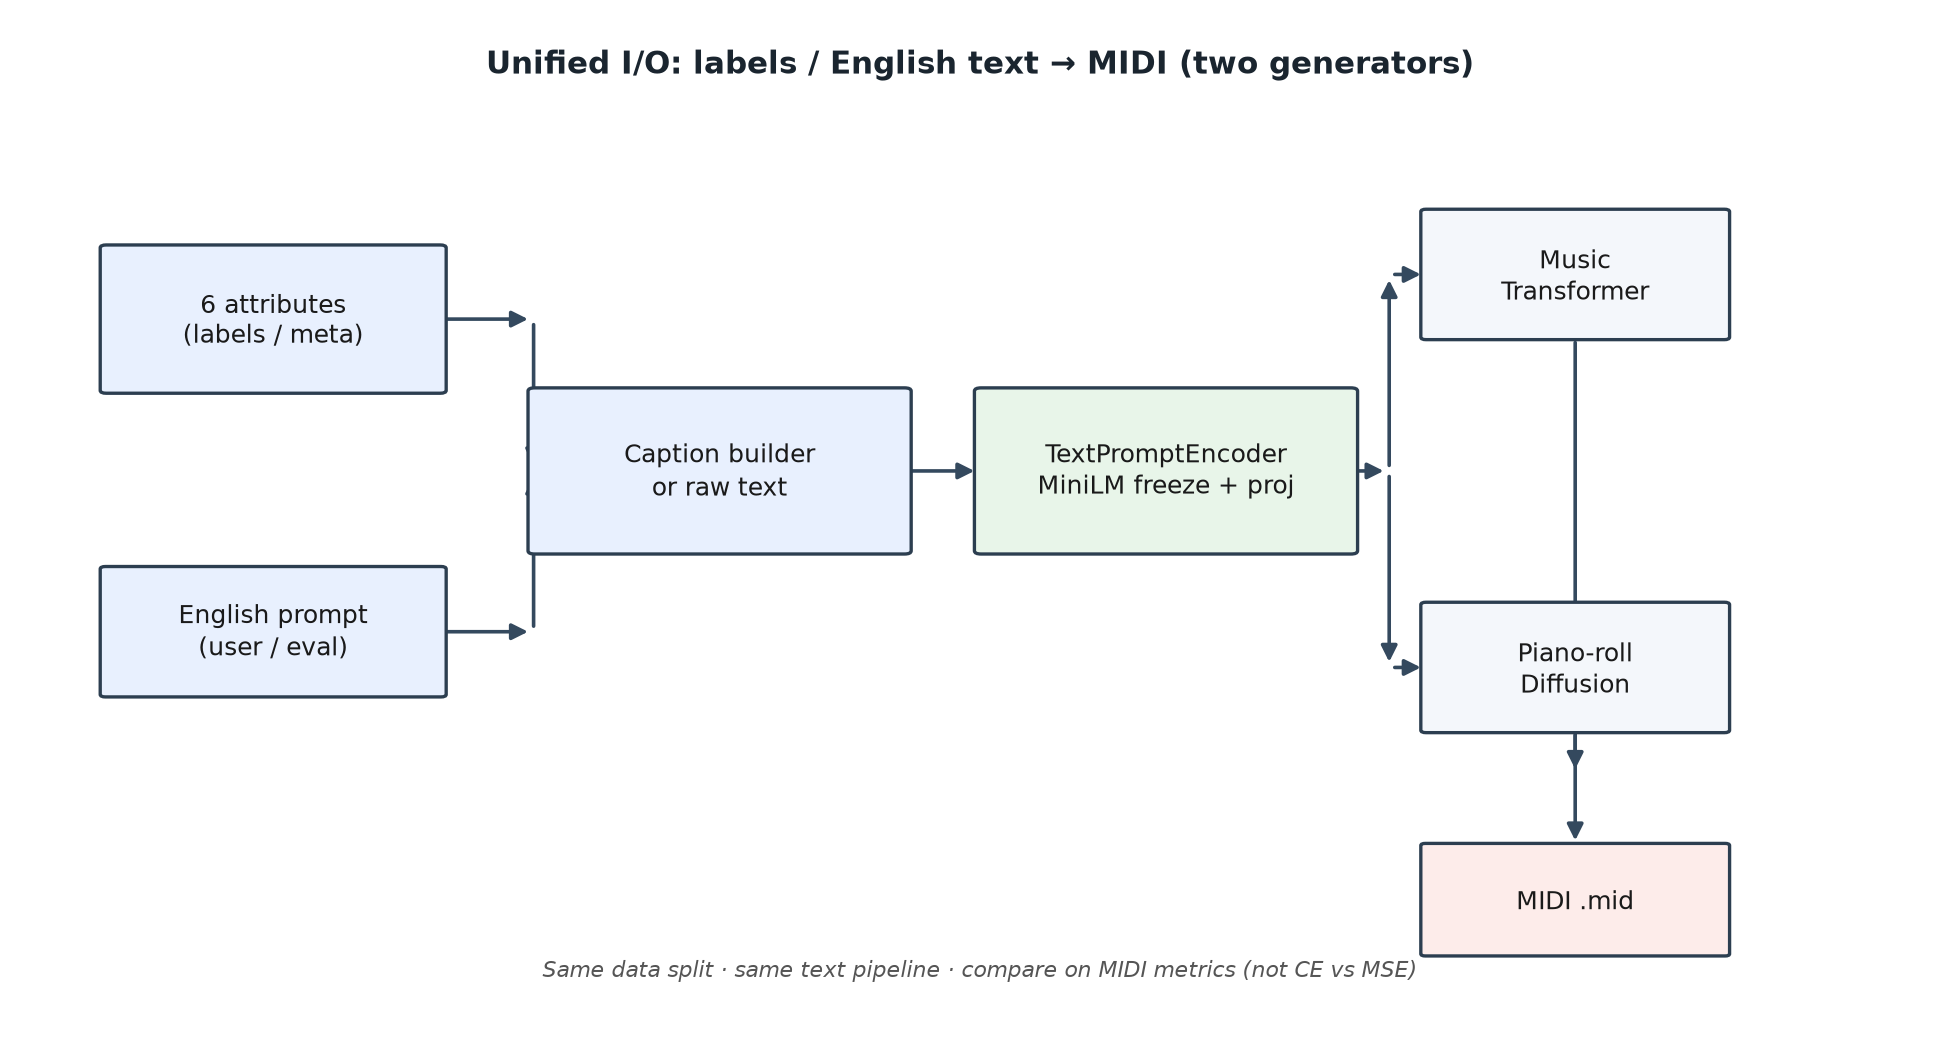
\includegraphics[width=0.95\textwidth]{system_overview_text}
    \caption{Kiến trúc tổng thể: cùng pipeline text$\rightarrow c$ (MiniLM đóng băng + projection),
    hai generator độc lập, đầu ra MIDI và so sánh bằng metric trên \texttt{compare/}.}
    \label{fig:ch3-system-arch}
\end{figure}

%------------------------------------------------------------------------------
\section{Chuẩn hóa đầu vào --- từ nhãn cấu trúc đến câu text}
\label{sec:ch3-prompt}

Hai nhánh chỉ so sánh được khi chúng nhận điều kiện theo cùng một quy ước. Đồ án tách rõ \textbf{lược đồ nhãn} (phía dữ liệu/đánh giá) và \textbf{biểu diễn điều kiện} (phía mô hình).

\subsection{Lược đồ sáu thuộc tính (tầng nhãn)}

Sáu thuộc tính và số lớp tham chiếu trong cấu hình YAML / tài liệu dữ liệu được tóm trong bảng~\ref{tab:ch3-prompt-schema}. Chúng xuất hiện trong \texttt{data/labels/labels.json}, trong meta của \texttt{eval\_prompts.json}, và trong logic chỉ số (ví dụ \texttt{instrument\_match}, \texttt{PROGRAM\_MAP} phía Diffusion).

\begin{table}[htbp]
\centering
\caption{Lược đồ thuộc tính có cấu trúc (nhãn / meta)}
\label{tab:ch3-prompt-schema}
\small
\begin{tabular}{lcc}
\toprule
Thuộc tính & Số lớp & Ví dụ nhãn \\
\midrule
mood & 10 & happy, sad, dark, epic, \ldots \\
genre & 10 & fantasy, horror, rpg, \ldots \\
scene & 10 & forest, dungeon, village, \ldots \\
tempo & 5 & slow, moderate, fast, \ldots \\
instrument & 8 & piano, strings, brass, guitar, \ldots \\
energy & 5 & calm, medium, intense, \ldots \\
\bottomrule
\end{tabular}
\end{table}

Trong mã nguồn còn module \texttt{compare/prompt\_schema.py} (ánh xạ nhãn$\leftrightarrow$ID) mang tính di sản từ thiết kế nhúng 6 ID cũ; \textbf{đường huấn luyện--sinh chính} của Transformer/Diffusion hiện tại \textbf{không} đưa sáu ID qua \texttt{nn.Embedding}, mà đi qua câu text (các mục tiếp theo).

\subsection{Sinh câu tiếng Anh từ nhãn (caption)}
\label{sec:ch3-caption}

Hàm \texttt{labels\_to\_english\_caption} trong \texttt{compare/caption.py} ghép sáu trường (đã chuẩn hóa chữ thường) thành một câu theo mẫu cố định, ví dụ:

\begin{center}
\textit{``happy fantasy village music, fast tempo, piano, medium energy''}.
\end{center}

Khi huấn luyện, mỗi mẫu MIDI ưu tiên caption có sẵn trong \texttt{captions.json} (nếu có và khác rỗng); nếu không, lấy nhãn từ \texttt{labels.json} rồi gọi \texttt{labels\_to\_english\_caption}. Khi đánh giá, \texttt{entry\_to\_prompt\_text} ưu tiên trường \texttt{text} (hoặc \texttt{prompt}) trong \texttt{eval\_prompts.json}; nếu thiếu thì ghép lại từ sáu thuộc tính. Bộ 20 câu eval được viết sẵn theo cùng khung nghĩa (mood--genre--scene--tempo--instrument--energy), nên phong cách gần với template huấn luyện, dù có thể khác chữ hoa/thường hoặc cách diễn đạt chi tiết so với chuỗi do hàm ghép sinh ra.

Việc dùng template có hai hệ quả. Thứ nhất, miền ngôn ngữ thực tế \textbf{hẹp} hơn text-to-music thương mại: mô hình chủ yếu thấy biến thể của cùng khung câu. Thứ hai, CLI suy luận vẫn nhận chuỗi \texttt{--prompt} tùy ý; chất lượng bám prompt ngoài phân phối template phụ thuộc khả năng tổng quát của MiniLM và projection đã học --- đồ án \textbf{không} khẳng định hiểu mọi mô tả tiếng Anh tự do.

\subsection{TextPromptEncoder: MiniLM đóng băng + projection}
\label{sec:ch3-text-encoder}

Lớp mã nguồn dùng chung nằm tại \texttt{compare/text\_conditioner.py}, được re-export bởi \texttt{prompt\_encoder.py} của cả hai nhánh dưới tên \texttt{TextPromptEncoder}. Luồng xử lý:

\begin{enumerate}
    \item Tokenizer và backbone \texttt{sentence-transformers/all-MiniLM-L6-v2} (thư viện HuggingFace \texttt{transformers}) mã hóa batch câu; lấy mean-pooling trên token có mask, rồi chuẩn hóa $\ell_2$, cho vector $384$ chiều.
    \item Backbone được \textbf{đóng băng} (\texttt{requires\_grad=False}, luôn ở chế độ eval): không cập nhật trọng số ngôn ngữ khi huấn luyện nhạc.
    \item Lớp chiếu học được: $\mathrm{Linear}(384\rightarrow d)\rightarrow\mathrm{GELU}\rightarrow\mathrm{LayerNorm}\rightarrow\mathrm{Linear}(d\rightarrow d)$ với $d=d_{\mathrm{model}}$ hoặc $d_{\mathrm{cond}}$ (thường $256$), cho ra vector điều kiện $c\in\mathbb{R}^{d}$.
    \item Module còn khai báo tham số \texttt{null\_emb}; tuy nhiên trong triển khai Diffusion hiện tại, \textbf{CFG / cond-drop dùng vector không} ($\mathbf{0}$), gán trực tiếp trong \texttt{\_maybe\_drop\_cond} và \texttt{predict\_noise}, chứ không gọi \texttt{null\_condition()}.
\end{enumerate}

Checkpoint lưu projection (và phần mạng nhạc); backbone MiniLM được tải lại từ HuggingFace lúc khởi tạo. Hai nhánh import cùng lớp encoder nên \textbf{cùng kiến trúc và cùng cách mã hóa câu}; sau huấn luyện, trọng số projection (và UNet/Transformer) của mỗi nhánh là độc lập.

\begin{table}[htbp]
\centering
\caption{Đối chiếu thiết kế điều kiện: phiên bản nhúng 6 ID (cũ) và text MiniLM (hiện tại)}
\label{tab:ch3-cond-evolution}
\small
\begin{tabular}{p{3.2cm}p{5.0cm}p{5.2cm}}
\toprule
\textbf{Hạng mục} & \textbf{Nhúng 6 ID (cũ)} & \textbf{Text MiniLM (hiện tại)} \\
\midrule
Đầu vào model & Sáu chỉ số nguyên & Câu English \\
Encoder & $6\times$ embedding + MLP & MiniLM freeze + projection \\
Train caption & Không cần câu & Template / \texttt{captions.json} \\
Suy luận & Chọn nhãn / ID & \texttt{--prompt "..."} hoặc ghép từ nhãn \\
Đồng bộ hai nhánh & Cùng schema ID & Cùng pipeline text; projection riêng \\
Hạn chế chính & Không nhận câu text & Template hẹp; MiniLM không fine-tune \\
\bottomrule
\end{tabular}
\end{table}

Thiết kế hiện tại đánh đổi như sau: giao diện gần text-to-music và tái sử dụng tri thức ngôn ngữ có sẵn của MiniLM; đổi lại, so sánh backbone tạo sinh vẫn kiểm soát được vì encoder text \textbf{cùng pipeline và đóng băng}, không tinh chỉnh một encoder ngôn ngữ khác nhau cho từng nhánh (projection thì học riêng theo từng bài toán CE hoặc MSE).

%------------------------------------------------------------------------------
\section{Dataset và tiền xử lý}
\label{sec:ch3-data}

\subsection{Kho dữ liệu dùng chung}

Thư mục \texttt{data/processed} chứa khoảng \textbf{14\,232} tệp MIDI sau bước lọc và gộp nguồn. Nhãn nằm tại \texttt{data/labels/labels.json}. Theo tài liệu dữ liệu của đồ án, thành phần chính là ComMU (cỡ \textbf{11\,144} tệp có siêu dữ liệu có cấu trúc), kèm phần MidiCaps và MAESTRO đã được đưa vào processed. Việc tách huấn luyện/kiểm định không để mỗi mô hình tự lấy mẫu ngẫu nhiên lại, mà dùng tệp cố định \texttt{compare/split.json}: khoảng \textbf{12\,809} mẫu huấn luyện và \textbf{1\,423} mẫu kiểm định (xấp xỉ 10\% kiểm định). Cả hai bộ huấn luyện đọc cùng danh sách này, nhờ đó khác biệt quan sát sau này không thể quy cho việc một bên quan sát tập khác bên kia.

\begin{figure}[htbp]
    \centering
    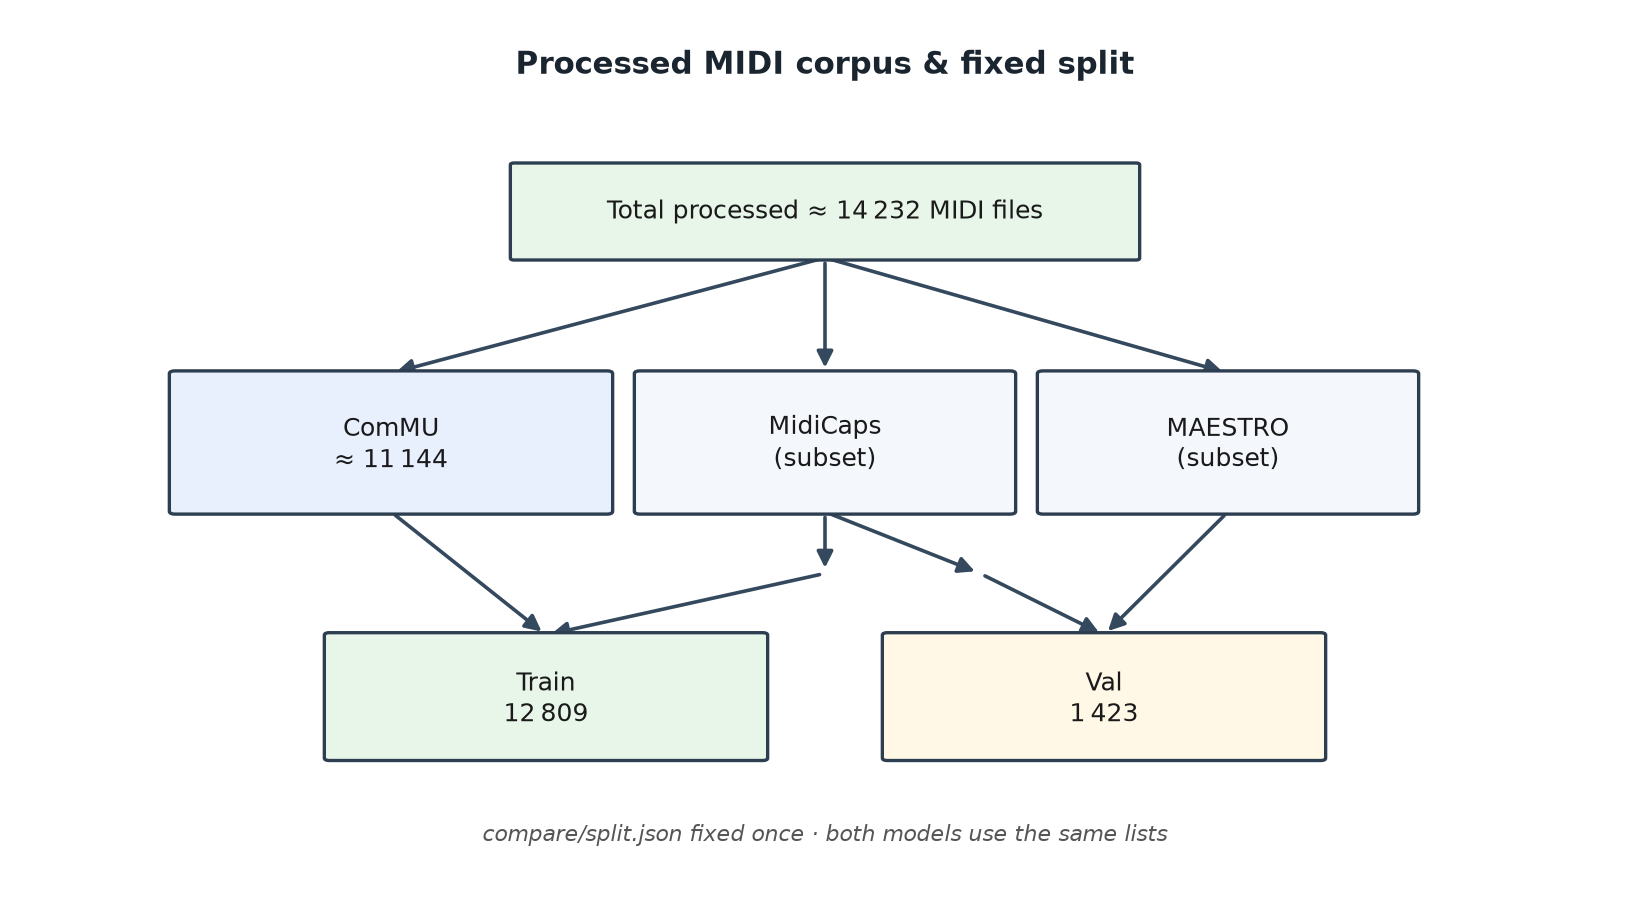
\includegraphics[width=0.85\textwidth]{fig_ch3_data_composition}
    \caption{Thành phần kho MIDI đã xử lý ($\approx$14\,232 tệp) và phân chia cố định
    huấn luyện/kiểm định trong \texttt{compare/split.json}.}
    \label{fig:ch3-data-composition}
\end{figure}

\subsection{Nhánh Transformer: tokenizer REMI}

Phía Transformer, \texttt{GenAI\_Transformer/src/data/tokenizer.py} mã hóa MIDI theo kiểu REMI-like. Chú thích trong mã ghi vocabulary khoảng \textbf{388} token, gồm nhóm đặc biệt (\texttt{<PAD>}, \texttt{<BOS>}, \texttt{<EOS>}, \texttt{<UNK>}), \texttt{NOTE\_ON}/\texttt{NOTE\_OFF} trên 88 pitch (21--108), 32 bin vận tốc, \texttt{TIME\_SHIFT} với bước 10\,ms (tối đa 1\,s mỗi token), tám bin tempo, và mười sáu nhóm instrument theo \texttt{program//8}.

Khi mã hóa, các nốt từ mọi track (bỏ drum) được gom và sắp theo thời gian; mỗi lần đổi nhóm nhạc cụ, tokenizer chèn token \texttt{INST\_*}. Chiều ngược lại quan trọng không kém: lúc giải mã (\texttt{decode}), token \texttt{INST\_*} cập nhật program hiện hành, còn nếu chuỗi không có \texttt{INST\_*} thì mặc định piano (program 0). Hệ quả trực tiếp là nhạc cụ trong tệp sinh \textbf{phải do mô hình quyết định qua token}. Chỉ số khớp instrument về sau, nếu đọc đúng, đang đo hành vi học chứ không đo một bước gán nhãn sau cùng.

Độ dài chuỗi bị chặn bởi \texttt{max\_seq\_len} (cấu hình có thể lên 2048; thực nghiệm so sánh thường dùng 1024 để cân VRAM và thông lượng, theo hướng dẫn huấn luyện của kho mã nguồn). Tokenizer còn giữ bộ nhớ đệm mã hóa giới hạn (mặc định 500 mục) nhằm giảm lặp đọc tệp khi duyệt nhiều epoch.

\subsection{Nhánh Diffusion: piano-roll}

Phía Diffusion, \texttt{GenAI\_Diffusion/src/data/pianoroll.py} biến MIDI thành lưới hai chiều: 88 pitch (21--108) nhân 256 frame tại 24\,Hz, tương đương khoảng $10{,}7$ giây. Vận tốc được chuẩn hóa, nén gamma $0{,}8$, rồi ánh xạ về $[-1,1]$. Khi huấn luyện, quy trình cắt ngẫu nhiên theo trục thời gian và dịch pitch trong khoảng $\pm 2$ bán cung. Điểm then chốt là nhiều track được gộp qua \texttt{get\_piano\_roll} thành \textbf{một kênh} duy nhất: giai điệu, hòa âm và bass, nếu có, chồng lên cùng mặt phẳng kích hoạt.

Hệ quả dự kiến --- và sẽ được đối chiếu bằng số liệu ở chương sau --- là mô hình học một trường 2D chứ không học tách stem. Mật độ nốt sau khi ra MIDI phụ thuộc mạnh vào cách ngưỡng hóa roll, không chỉ vào việc MSE đã thấp hay chưa.

% Chi tiết mã hóa piano-roll: xem Mục~\ref{sec:ch3-diff-decode} và
% Hình~\ref{fig:ch2-pianoroll-limits} (hạn chế lưới một kênh).

%------------------------------------------------------------------------------
\section{Triển khai Music Transformer}
\label{sec:ch3-transformer}

\subsection{Kiến trúc}
\begin{figure}[htbp]
    \centering
    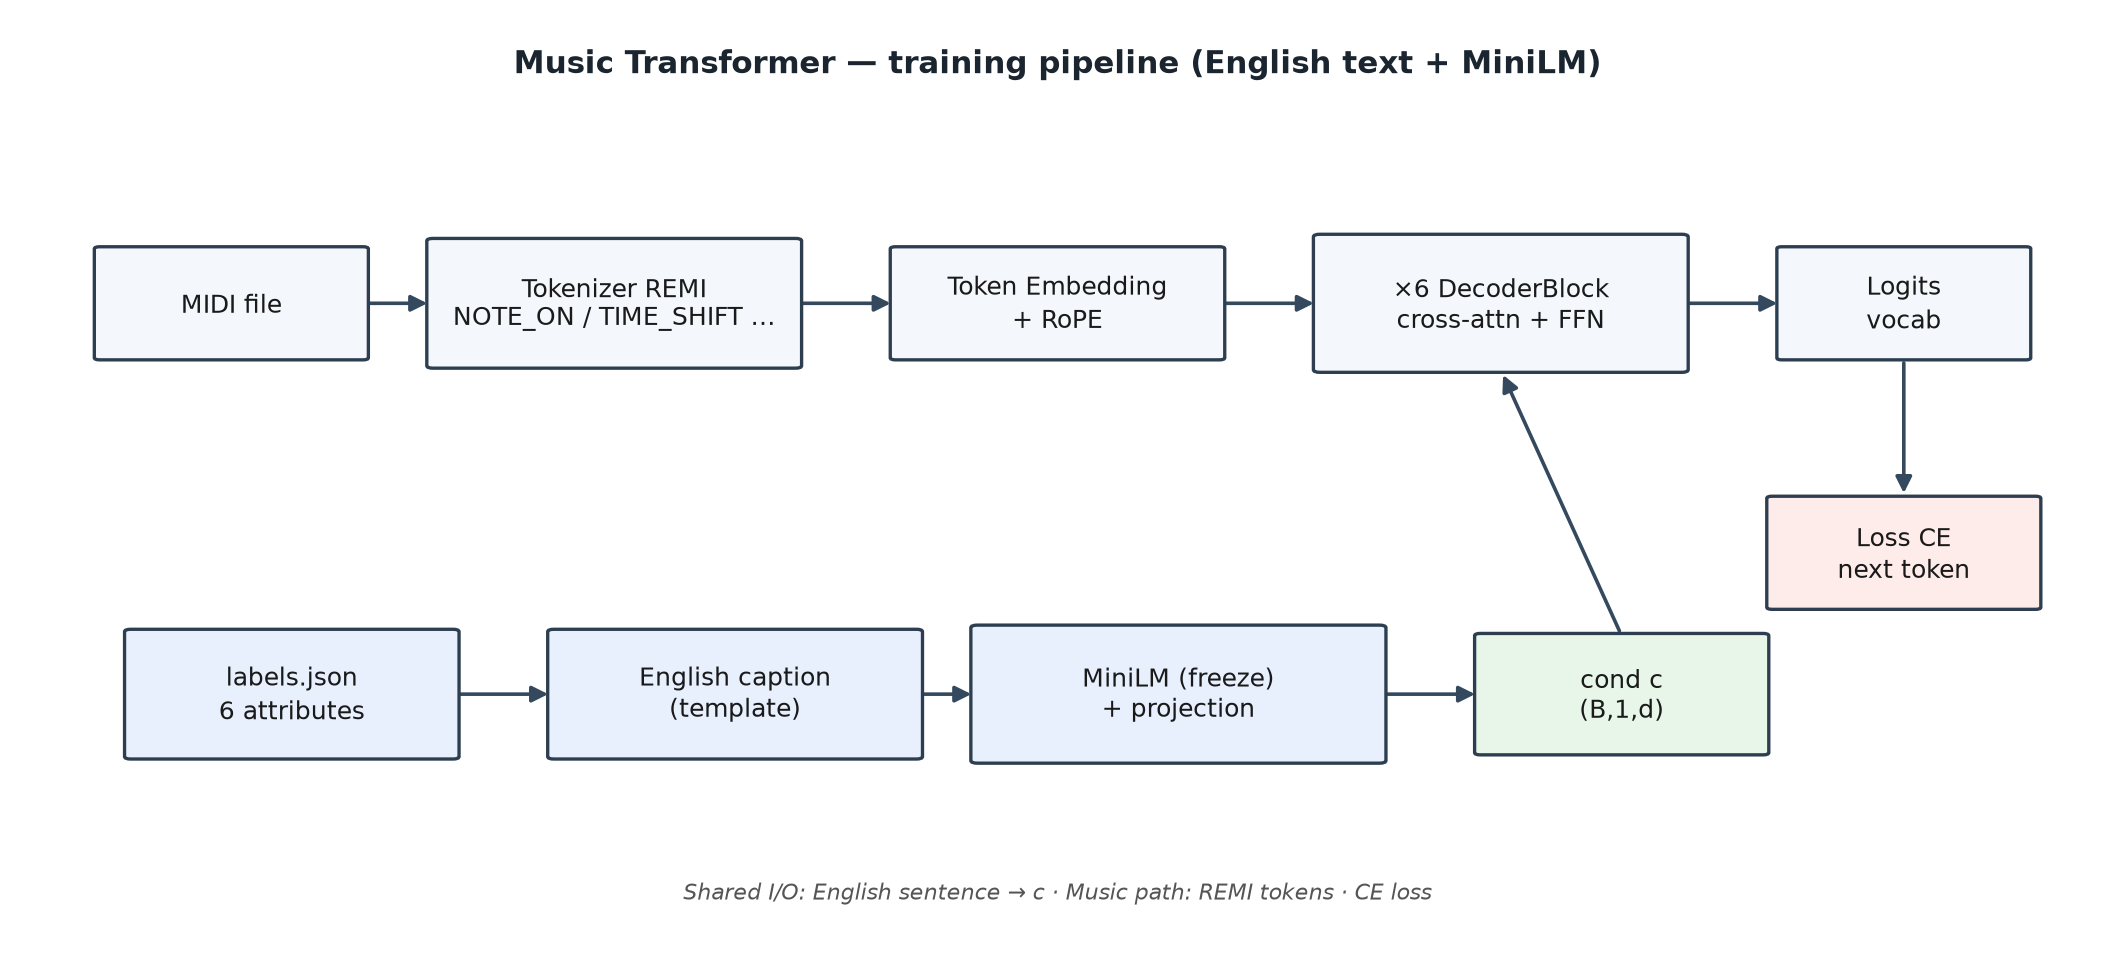
\includegraphics[width=0.95\textwidth]{transformer}
    \caption{Luồng huấn luyện Music Transformer: REMI tokens + CE; điều kiện text qua
    MiniLM đóng băng + projection $\rightarrow$ cross-attention.}
    \label{fig:ch3-transformer-train}
\end{figure}

\begin{figure}[htbp]
    \centering
    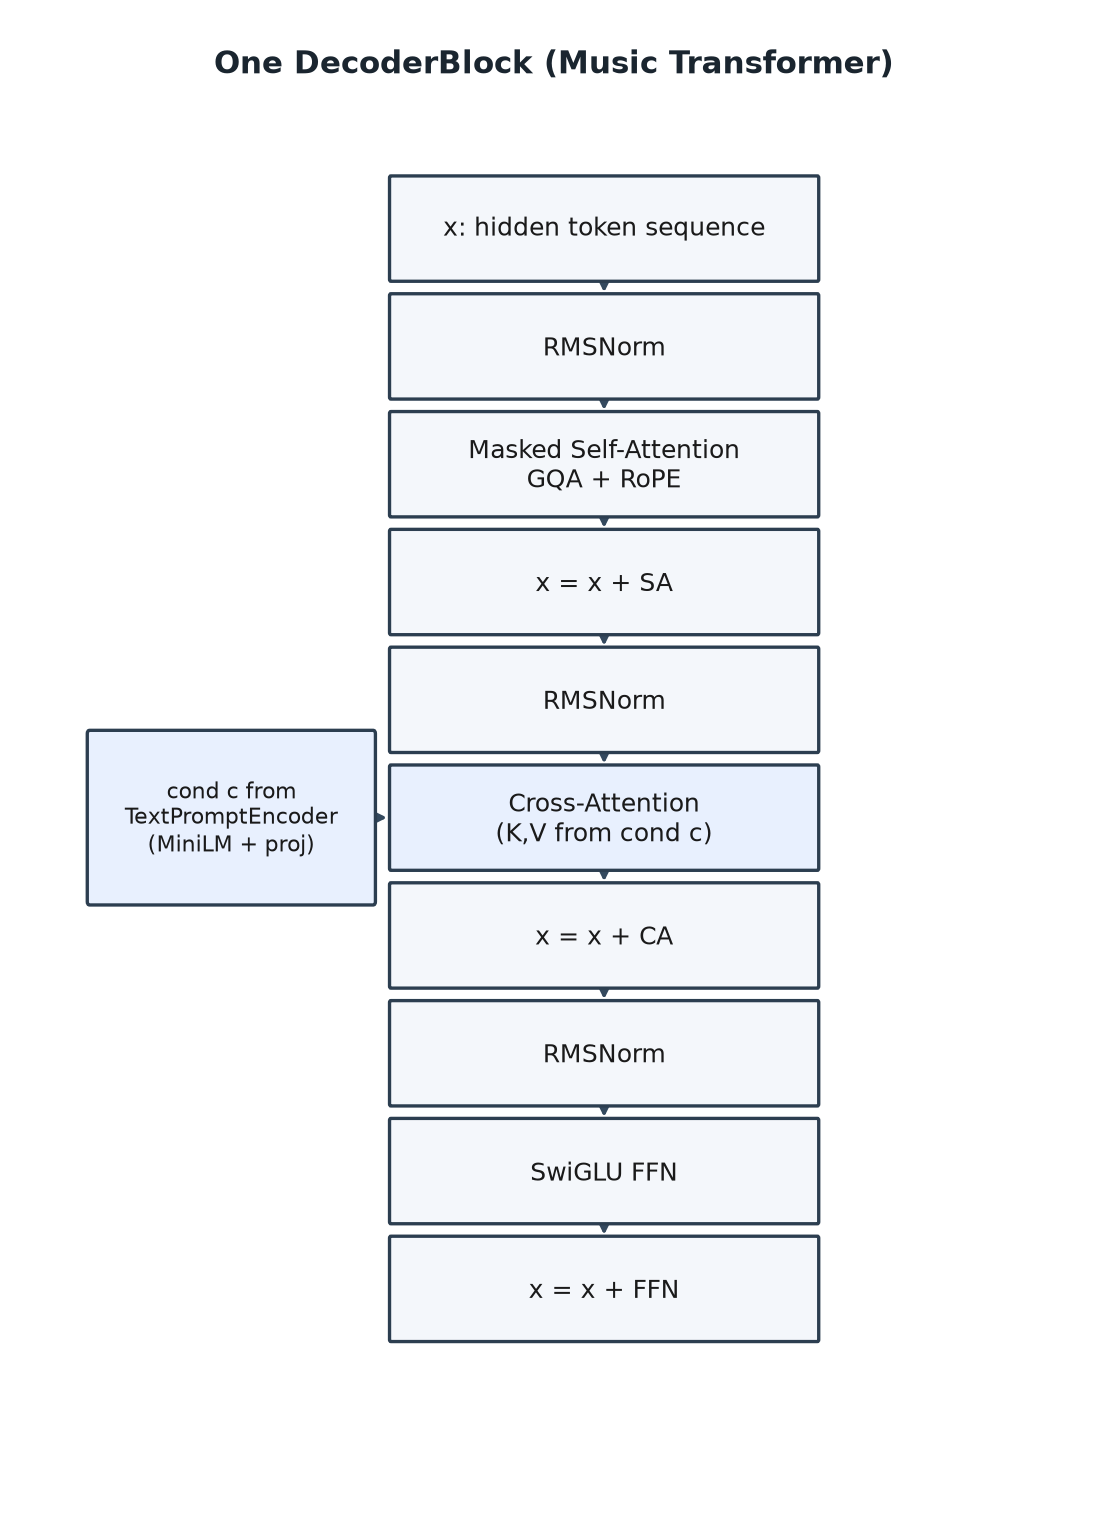
\includegraphics[width=0.48\textwidth]{decoder-block}
    \caption{Một \texttt{DecoderBlock}: self-attention nhân quả (GQA+RoPE),
    cross-attention với $c$ text, SwiGLU FFN (Pre-Norm / RMSNorm).}
    \label{fig:ch3-decoder-block}
\end{figure}

Lớp \texttt{MusicTransformer} trong \texttt{src/model/transformer.py} ghép bốn khối chính. \texttt{TextPromptEncoder} (Mục~\ref{sec:ch3-text-encoder}) nhận batch câu English và trả tensor điều kiện hình $(B,1,d_{\mathrm{model}})$ cho cross-attention. Token REMI đi qua \texttt{TokenEmbedding}. Tiếp theo là $N=6$ \texttt{DecoderBlock}, mỗi block lần lượt self-attention nhân quả, cross-attention với điều kiện, rồi FFN kiểu SwiGLU, theo kiểu Pre-Norm với RMSNorm. Đầu ra là lớp tuyến tính lên vocabulary; trọng số được \textbf{chia sẻ} (\textit{weight tying}) với embedding token.

Cấu hình mặc định trong \texttt{config/config.yaml} chọn $d_{\mathrm{model}}=256$, tám head, GQA với bốn KV head, $d_{\mathrm{ff}}=1024$, dropout $0{,}1$, và bật QK-Norm. Nhật ký so sánh chính ghi nhận khoảng \textbf{7{,}72\,M} tham số trainable (không tính backbone MiniLM đóng băng). Self-attention (\texttt{attention.py}) dùng RoPE, GQA, QK-Norm và phép nhân attention tường minh, một lựa chọn nhằm tránh một số lỗi SDPA trên driver GPU phổ thông. Cross-attention lấy $K,V$ từ điều kiện có độ dài đúng bằng một.

\subsection{Conditioning}

Mọi lớp decoder thực hiện cross-attention vào cùng một vector điều kiện toàn cục $c$ suy ra từ câu text (Mục~\ref{sec:ch3-text-encoder}). Cách làm này đơn giản và đồng bộ nguồn $c$ với nhánh Diffusion, nhưng cũng có hạn chế rõ: toàn bộ ngữ nghĩa câu bị nén vào \textbf{một} khe biểu diễn. Không có chuỗi token điều kiện tách mood / instrument / \ldots, nên mô hình không được nhắc tường minh theo từng thuộc tính tại mỗi vị trí thời gian.

\subsection{Hàm mất mát và huấn luyện}

Huấn luyện theo teacher forcing: tại mỗi bước, mô hình dự đoán $y_t$ từ $y_{<t}$ và điều kiện $c$ (câu caption đã encode). Hàm mất mát là \texttt{CrossEntropyLoss} với \texttt{ignore\_index} bằng token pad và \textbf{làm mượt nhãn} $0{,}1$. Bộ tối ưu AdamW dùng $\beta=(0{,}9,0{,}98)$ và weight decay $0{,}01$; gradient chỉ cập nhật mạng nhạc và projection text, không cập nhật MiniLM. Lịch learning rate gồm warmup chiếm khoảng $5\%$ tổng số bước, sau đó cosine decay. Gradient được tích lũy (thường bốn bước micro-batch), cắt chuẩn $\ell_2$ với ngưỡng $1{,}0$, và huấn luyện dưới AMP khi có CUDA. Bộ huấn luyện còn khôi phục trọng số nếu gặp logits, hàm mất mát hoặc gradient không hữu hạn --- cơ chế thực dụng khi chuỗi dài trên GPU phổ thông. Nhật ký được ghi vào \texttt{compare/results/transformer\_training.csv}; điểm kiểm tra tốt nhất chọn theo entropy chéo kiểm định, đồng thời lưu thêm các mốc epoch phục vụ so sánh dọc quá trình học. Độ bối rối trên tập kiểm định được tính $\mathrm{PPL}=\exp(\mathcal{L}_{\mathrm{val}})$, có kẹp số học trong mã nguồn khi hàm mất mát lớn.

Một vòng batch diễn ra như sau. Lấy tokens và câu caption (từ nhãn/caption file); tách input $[:,:-1]$ và target $[:,1:]$; encode text $\rightarrow c$; bỏ batch nếu số token khác pad quá ít; lan truyền xuôi dưới AMP; entropy chéo trên logits phẳng; chia hàm mất mát cho số bước tích lũy; lan truyền ngược; đủ micro-step thì unscale (nếu AMP), cắt gradient, cập nhật bộ tối ưu và lịch learning rate. Các bước an toàn số học nhằm tránh một batch lỗi làm hỏng cả điểm kiểm tra.

\subsection{Sinh mẫu}

\texttt{MusicGenerator} (\texttt{inference/generator.py}) mã hóa câu English một lần thành $c$, rồi sinh token tự hồi quy kèm KV-cache cho đến \texttt{EOS} hoặc \texttt{max\_length}. Điểm vào CLI (\texttt{generate.py}) nhận \texttt{--prompt} dạng chuỗi; nếu chỉ có các cờ nhãn có cấu trúc thì ghép caption bằng \texttt{labels\_to\_english\_caption}. Hàm \texttt{combined\_sampling} (\texttt{sampling.py}) áp temperature mặc định $0{,}85$, top-$p$ mặc định $0{,}9$, còn top-$k$ tắt theo mặc định. Chuỗi ID cuối cùng qua \texttt{tokenizer.decode} thành đối tượng \texttt{PrettyMIDI} và được ghi ra đĩa.

%------------------------------------------------------------------------------
\section{Triển khai Piano-roll Diffusion}
\label{sec:ch3-diffusion}

\begin{figure}[htbp]
    \centering
    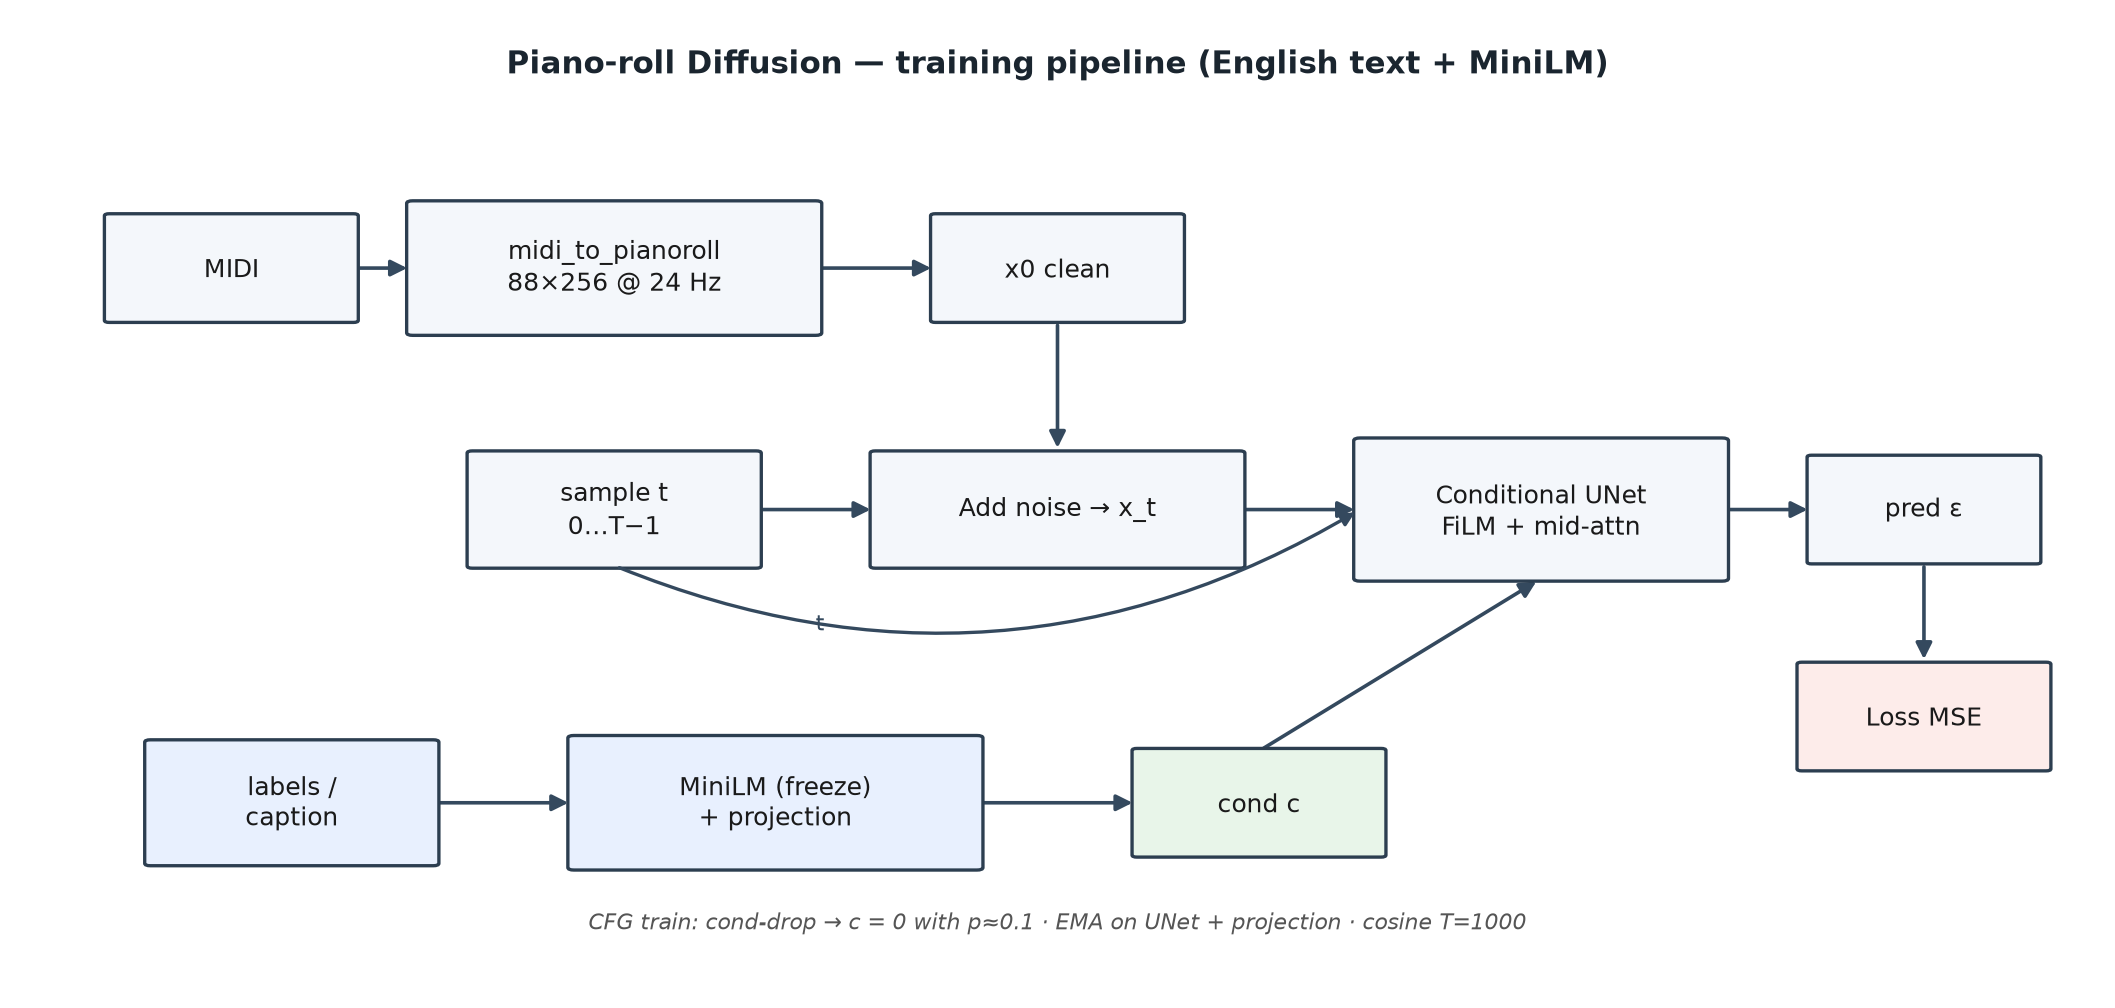
\includegraphics[width=0.95\textwidth]{train-diffusion}
    \caption{Luồng huấn luyện Piano-roll Diffusion: MIDI$\rightarrow$roll $88\times 256$,
    nhiễu theo $t$, UNet có FiLM từ $c$ text, mất mát MSE; cond-drop cho CFG và EMA.}
    \label{fig:ch3-diffusion-train}
\end{figure}

\begin{figure}[htbp]
    \centering
    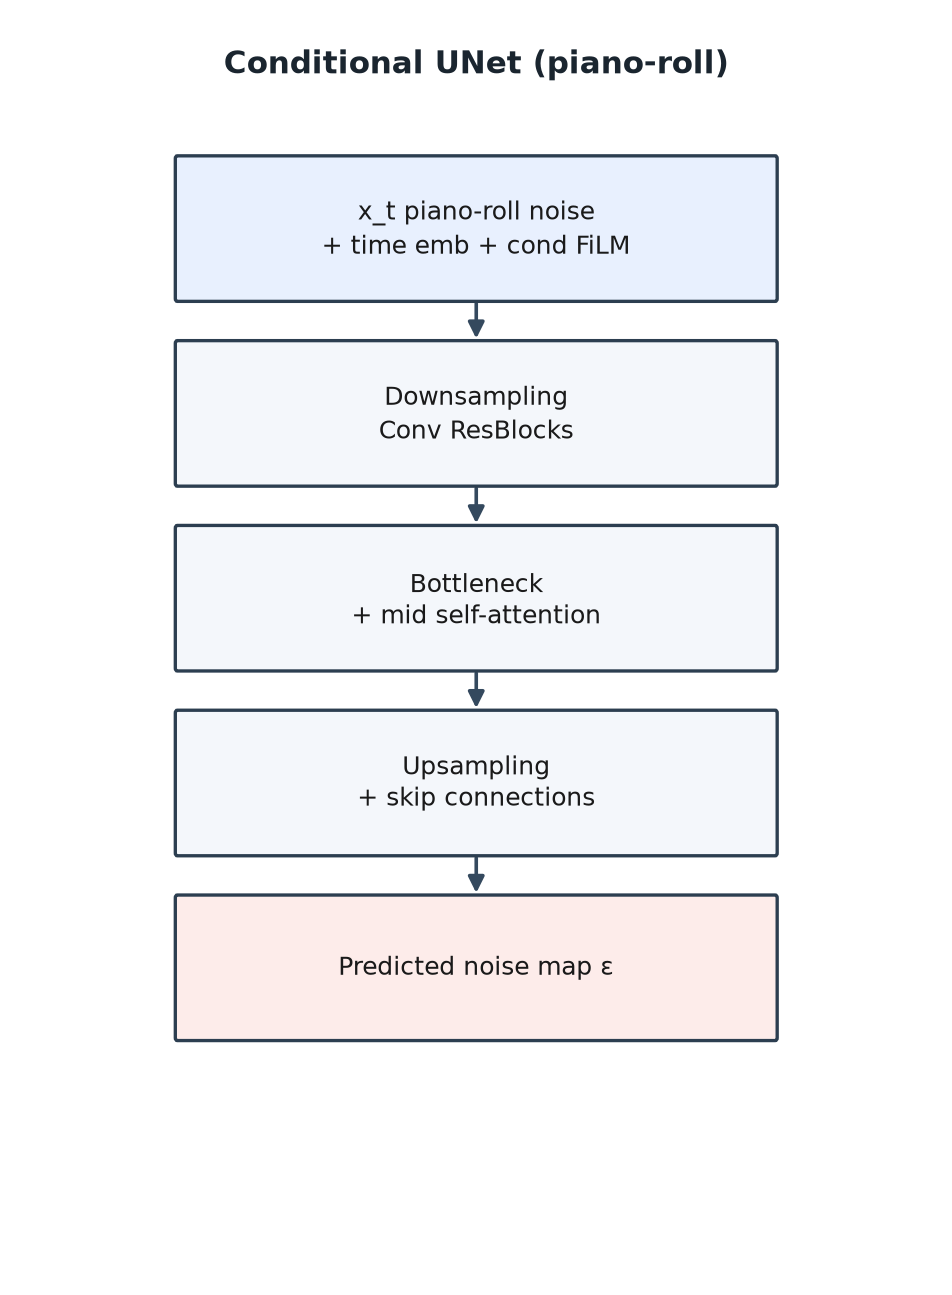
\includegraphics[width=0.42\textwidth]{unet}
    \caption{Conditional UNet trên piano-roll: down/up ResBlock, mid self-attention,
    điều chế time emb + cond $c$ kiểu FiLM, đầu ra bản đồ nhiễu $\epsilon$.}
    \label{fig:ch3-unet}
\end{figure}

\subsection{Kiến trúc}

Nhánh diffusion cũng bắt đầu từ \texttt{TextPromptEncoder} (cùng pipeline MiniLM + projection như nhánh Transformer, trọng số projection độc lập), nhưng đầu ra là vector $(B,d_{\mathrm{cond}})$ chứ không unsqueeze thành chuỗi. \texttt{ConditionalUNet} (\texttt{unet.py}) gồm stem convolution, các ResBlock down/up, và self-attention 2D ở mid-block. Mỗi ResBlock điều chế đặc trưng theo kiểu \textbf{FiLM}: scale và shift được suy ra từ biểu diễn nhúng thời gian và từ điều kiện $c$, rồi cộng lại trước khi chuẩn hóa. Lớp \texttt{GaussianDiffusion} (\texttt{diffusion.py}) quản lý lịch cosine với $T=1000$, các hàm \texttt{q\_sample}, \texttt{p\_losses}, lấy mẫu DDIM và CFG. Trên UNet và projection text còn có \textbf{EMA} với hệ số suy giảm $0{,}999$.

Cấu hình chất lượng trong \texttt{config/config.yaml} đặt \texttt{base\_channels=64}, channel mults $[1,2,4]$, \texttt{cond\_dim=256}, \texttt{sample\_steps=80}, \texttt{guidance\_scale=3.5}, $\eta=0$. Tóm tắt mô hình của thực nghiệm so sánh chính ghi khoảng \textbf{4{,}43\,M} tham số. Các lần thử trước từng xuất hiện cấu hình khoảng $13{,}7$\,M; phần phân tích kết quả ở chương sau bám điểm kiểm tra và nhật ký của thực nghiệm đủ 30 epoch trên toàn bộ phân chia, không trộn với các thử nghiệm quy mô tham số khác.

\subsection{Conditioning và CFG}

Trong lúc huấn luyện, \texttt{\_maybe\_drop\_cond} gán $c\leftarrow\mathbf{0}$ với xác suất $0{,}1$ (cond-drop), buộc UNet học cả nhánh có điều kiện lẫn vô điều kiện trên không gian vector đã chiếu. Khi lấy mẫu, \texttt{predict\_noise} kết hợp hai dự đoán theo

\[
\tilde\epsilon
=
\epsilon_{\emptyset}
+
s\,(\epsilon_{c}-\epsilon_{\emptyset}),
\]

với $s$ mặc định $3{,}5$ và $\epsilon_{\emptyset}$ ứng với điều kiện \textbf{vector không} $\mathbf{0}$ (không dùng \texttt{null\_emb} trong đường CFG hiện tại). FiLM đưa $c$ vào mọi ResBlock ở mức toàn cục; không có cross-attention giữa prompt và từng vị trí không gian trên roll.

\subsection{Hàm mất mát và huấn luyện}

\texttt{p\_losses} thêm nhiễu vào $x_0$, để UNet dự đoán $\epsilon$, rồi tối thiểu hóa \textbf{MSE}. Không có hạng tử thưa hóa, cũng không có hàm mất mát phụ cho instrument. Bộ huấn luyện (\texttt{training/trainer.py}) dùng AdamW với learning rate cấu hình $1{,}5\times 10^{-4}$; trong nhật ký thực nghiệm 30 epoch đầy đủ, learning rate được ghi nhận \textbf{không giảm dần}, giữ cố định $1{,}5\times 10^{-4}$. AMP, tích lũy gradient, cắt chuẩn và cập nhật EMA sau mỗi bước tối ưu được bật. Kiểm định đo MSE trung bình với trọng số EMA shadow và ghi \texttt{diffusion\_training.csv}.

Lớp \texttt{EMA} (\texttt{src/model/ema.py}) giữ bản sao floating-point của tham số và cập nhật
$\theta_{\mathrm{shadow}} \leftarrow \alpha\theta_{\mathrm{shadow}} + (1-\alpha)\theta$
với $\alpha=0.999$. Khi đánh giá hoặc lấy mẫu, \texttt{apply\_shadow} ghi đè tạm trọng số mô hình rồi \texttt{restore}. Điểm kiểm tra \texttt{best\_model.pt} phía diffusion được lưu với tùy chọn dùng trọng số EMA, nhất quán với thực hành phổ biến nhằm ổn định mẫu.

Một bước huấn luyện gồm: lấy piano-roll $x_0$ và câu caption, mã hóa $c$ bằng \texttt{TextPromptEncoder}, lấy mẫu $t$ đều trong $\{0,\ldots,T-1\}$, tính \texttt{p\_losses} (có thể drop $c$), lan truyền ngược/tích lũy, cắt gradient rồi AdamW (MiniLM đóng băng), cuối cùng cập nhật EMA. Kiểm định lặp lại MSE trên bộ nạp dữ liệu kiểm định với trọng số shadow.

\subsection{Sinh mẫu và giải mã MIDI}
\label{sec:ch3-diff-decode}

\texttt{generate.py} nhận câu \texttt{--prompt}, encode thành $c$, rồi gọi \texttt{diffusion.sample} theo DDIM ($\eta=0$, số bước lấy từ config hoặc CLI). Sau khi có roll, quy trình không để ``nhạc cụ'' cho UNet tự quyết theo nghĩa program MIDI. Thay vào đó, \texttt{program} được lấy từ \texttt{PROGRAM\_MAP} theo nhãn \texttt{instrument} trong meta prompt (ví dụ piano ánh xạ 0, strings ánh xạ 48) --- tách biệt với việc $c$ text đã vào UNet qua FiLM. Hàm \texttt{pianoroll\_to\_midi} ánh xạ $[-1,1]$ về $[0,1]$, áp ngưỡng (mặc định $0{,}15$, có chỉnh theo phân vị của các kích hoạt dương), loại bỏ các đoạn kích hoạt ngắn, ép thời lượng tối thiểu, rồi ghi đúng \textbf{một} track \texttt{Instrument(program=...)}. Nếu gần như không còn nốt, giải mã hạ ngưỡng lần hai để tránh mẫu rỗng.

Hệ quả bắt buộc phải mang sang chương thực nghiệm: trong \texttt{compare/midi\_metrics.py}, \texttt{instrument\_match} dựa trên program trội của tệp MIDI. Với Diffusion, program đến từ bảng ánh xạ nhãn instrument, nên chỉ số này \textbf{không phản ánh} việc UNet đã học âm sắc từ câu text hay chưa. Đây không phải lỗi chỉ số đơn thuần, mà là hệ quả thiết kế giải mã đã chọn.

\begin{figure}[htbp]
    \centering
    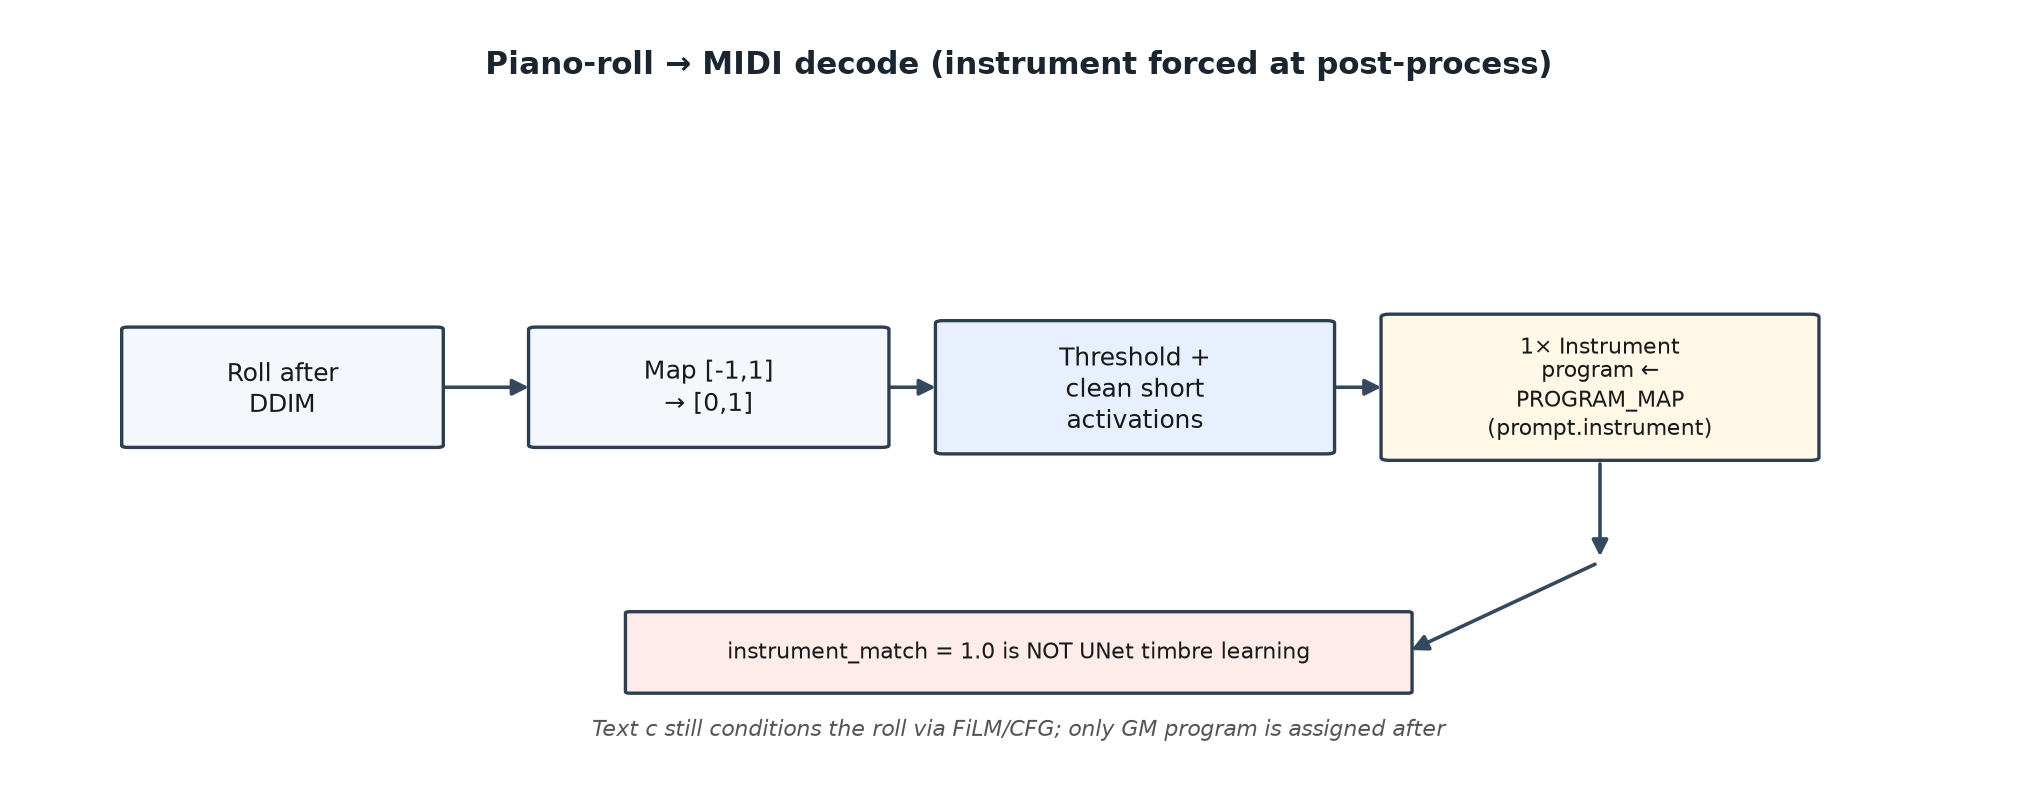
\includegraphics[width=0.95\textwidth]{fig_ch3_diffusion_decode}
    \caption{Giải mã piano-roll $\rightarrow$ MIDI: ngưỡng hóa và gán
    \texttt{program} từ \texttt{PROGRAM\_MAP} theo nhãn instrument ---
    \texttt{instrument\_match}${}=1$ không phản ánh học âm sắc của UNet.}
    \label{fig:ch3-diff-decode}
\end{figure}

%------------------------------------------------------------------------------
\section{So sánh thiết kế kỹ thuật}
\label{sec:ch3-design-compare}

Bảng~\ref{tab:ch3-design} tóm tắt các khác biệt triển khai then chốt. Đây là khung đọc cho Chương~\ref{chap:experiments}: hai hàm mất mát không cùng thang đo, và mọi so sánh chất lượng MIDI phải kèm hiểu biết về đường đi instrument cũng như giải mã.

\begin{table}[htbp]
\centering
\caption{Đối chiếu thiết kế hai nhánh như đã triển khai}
\label{tab:ch3-design}
\small
\begin{tabular}{p{2.8cm}p{5.5cm}p{5.5cm}}
\toprule
\textbf{Hạng mục} & \textbf{Transformer} & \textbf{Diffusion} \\
\midrule
Biểu diễn & Token REMI & Roll $1\times 88\times T$ \\
Nguồn điều kiện & Câu English + MiniLM + proj (riêng) & Cùng pipeline; proj riêng \\
Chèn $c$ vào net & Cross-attn, độ dài cond $=1$ & FiLM + CFG ($\mathbf{0}$) \\
Hàm mất mát & CE + làm mượt nhãn $0{,}1$ & MSE nhiễu \\
Lịch LR & Warmup + cosine & Cố định (thực nghiệm chính) \\
Lấy mẫu & AR, $\tau$+top-$p$ & DDIM 80, $s{=}3.5$ \\
Nhạc cụ & Token \texttt{INST\_*} & \texttt{PROGRAM\_MAP} lúc giải mã \\
Số tham số (nhật ký) & $\approx 7{,}72$\,M & $\approx 4{,}43$\,M \\
\bottomrule
\end{tabular}
\end{table}

%------------------------------------------------------------------------------
\section{Mô-đun đánh giá và so sánh}
\label{sec:ch3-eval}

Mô-đun \texttt{compare/} được thiết kế như lớp độc lập với hai bộ huấn luyện. Tệp \texttt{split.json} và \texttt{eval\_prompts.json} (20 mục, mỗi mục có trường \texttt{text} tiếng Anh kèm meta sáu thuộc tính) cố định đầu vào của vòng đánh giá. Mỗi phương pháp tại mỗi mốc epoch sinh MIDI vào \texttt{compare/outputs/} từ đúng câu \texttt{text}. \texttt{midi\_metrics.py} tính các đại lượng cấu trúc --- thời lượng, số nốt, mật độ, đa âm, tỉ lệ im lặng, tỉ lệ mẫu rỗng, thống kê pitch, histogram pitch-class và khoảng cách JS so với tham chiếu, \texttt{instrument\_match} (dựa meta \texttt{instrument}) --- cùng thời gian suy luận ghi nhận được. Các tệp tổng hợp như \texttt{quality\_summary.csv}, \texttt{comparison\_table.csv} và nhật ký huấn luyện từng nhánh cho phép tái lập bảng số của chương sau.

Cách diễn giải chỉ số được gắn sẵn vào thiết kế báo cáo. Entropy chéo không dùng để xếp Diffusion. \texttt{instrument\_match}${}=1$ ở Diffusion không được diễn giải là bám instrument hoàn hảo theo nghĩa tạo sinh. Thời lượng mặc định của diffusion khoảng $10{,}7$ giây, trong khi Transformer theo EOS hoặc độ dài chuỗi, nên so mật độ tuyệt đối giữa hai nhánh cần kèm nhận thức về khác độ dài đoạn.

%------------------------------------------------------------------------------
\section{Môi trường triển khai}
\label{sec:ch3-env}

Thực nghiệm được ghi nhận trên Linux với GPU \textbf{NVIDIA GeForce RTX~3060} (VRAM tổng khoảng 12\,GB theo \texttt{model\_summary.csv}), Python 3.12 và PyTorch CUDA. Điểm vào huấn luyện và sinh là \texttt{train.py}, \texttt{generate.py}, cùng \texttt{generate\_eval.py} phía Transformer. Siêu tham số điều khiển qua YAML và CLI (epoch, batch, learning rate). Hạt giống ngẫu nhiên mặc định trong config là 42. Chi tiết vận hành nằm trong \texttt{docs/TRAINING\_GUIDE.md} của kho mã nguồn.

%------------------------------------------------------------------------------
\section{Hạn chế của phần triển khai}
\label{sec:ch3-limits}

Một số hạn chế không phải sự cố bất ngờ mà là hệ quả của các lựa chọn trên, và sẽ được đối chiếu trực tiếp với số liệu ở chương sau. Câu caption huấn luyện chủ yếu theo template hẹp; MiniLM đóng băng nên không thích ứng miền nhạc; $c$ vẫn chỉ một vector toàn cục cho cross-attention/FiLM. Nhánh Diffusion dùng roll một kênh, hàm mất mát MSE thuần, giải mã thiên về giữ nốt, và gán program cố định từ nhãn. Nhánh Transformer phụ thuộc việc sinh \texttt{INST\_*} và \texttt{EOS}, với cross-attention mang thiên lệch toàn cục. Quy trình đánh giá chính chưa có thử nghiệm nghe, FAD hay CLAP score. CSV lịch sử còn sót các lần chạy thử trên tập con nhỏ (kiểm định NaN); phân tích chính chỉ bám thực nghiệm đủ dữ liệu 30 epoch.

%------------------------------------------------------------------------------
\section*{Tóm tắt chương}
\addcontentsline{toc}{section}{Tóm tắt chương}

Chương này đã mô tả quy trình dùng chung, cầu nối nhãn$\rightarrow$câu English$\rightarrow$\texttt{TextPromptEncoder}, cách REMI và piano-roll được tạo ra, kiến trúc kèm điều kiện hóa, hàm mất mát, huấn luyện và suy luận của hai nhánh, vai trò của \texttt{compare/}, môi trường RTX~3060, và các hạn chế triển khai then chốt --- đặc biệt đường đi của instrument và sự khác bản chất giữa entropy chéo và MSE. Chương~\ref{chap:experiments} đặt các quyết định đó cạnh nhật ký huấn luyện và chỉ số MIDI để xem giả thuyết thiết kế đứng vững đến đâu.

\chapter{Kết quả thực nghiệm và đánh giá}
\label{chap:experiments}

Chương này đưa ba câu hỏi RQ1--RQ3 ở Chương~\ref{chap:intro} xuống mặt số liệu. Nguồn chính là nhật ký huấn luyện và các chỉ số MIDI trong \texttt{compare/results/}, đọc trong bối cảnh thiết kế mã nguồn đã mô tả ở Chương~\ref{chap:implementation}. Các nhận định dừng ở cấu trúc sự kiện và hành vi học; khi chưa có đánh giá nghe có kiểm soát, báo cáo không suy diễn chất lượng cảm nhận.

%------------------------------------------------------------------------------
\section{Thiết lập thực nghiệm}
\label{sec:ch4-setup}

Thực nghiệm so sánh dựng trên cùng kho đã xử lý khoảng \textbf{14\,232} MIDI, với phân chia cố định \textbf{12\,809} huấn luyện / \textbf{1\,423} kiểm định trong \texttt{compare/split.json}. Điều kiện hóa dùng \textbf{cùng} module \texttt{TextPromptEncoder} (câu English $\rightarrow$ MiniLM đóng băng + projection); khi huấn luyện, câu được sinh từ nhãn sáu thuộc tính theo template. Vòng đánh giá sinh lặp lại \textbf{20} câu trong \texttt{eval\_prompts.json} (trường \texttt{text}, kèm meta thuộc tính cho chỉ số) tại các điểm kiểm tra epoch \textbf{1, 5, 10, 20, 30}.

Thông tin thực nghiệm đầy đủ trên phân chia này, trích từ \texttt{model\_summary.csv} và các tệp \texttt{*\_training.csv}, được tóm trong bảng~\ref{tab:ch4-setup}.

\begin{table}[htbp]
\centering
\caption{Thông tin thực nghiệm so sánh chính (trích nhật ký)}
\label{tab:ch4-setup}
\small
\begin{tabular}{lcc}
\toprule
 & \textbf{Transformer} & \textbf{Diffusion} \\
\midrule
Số tham số (triệu) & 7.717 & 4.433 \\
Thiết bị & CUDA, RTX 3060 & CUDA, RTX 3060 \\
Mẫu huấn luyện / kiểm định & 12809 / 1423 & 12809 / 1423 \\
Tích lũy gradient (nhật ký) & 4 & 4 \\
Kích thước batch (các dòng tóm tắt) & 2--8 & 1--4 \\
EMA & -- & Có \\
Số bước khuếch tán (lịch) & -- & 1000 \\
Số epoch phân tích & 30 (kiểm định ổn định từ ep.\ 2) & 30 \\
\bottomrule
\end{tabular}
\end{table}

Trước khi đọc đường cong hàm mất mát cần một bước làm sạch nhật ký. Cả \texttt{transformer\_training.csv} lẫn \texttt{diffusion\_training.csv} còn sót các dòng chạy thử trên tập con nhỏ (kiểm định \texttt{nan}, hàm mất mát cao bất thường). Phần hội tụ dưới đây chỉ giữ thực nghiệm chính: với Transformer là các epoch có \texttt{val\_loss} hợp lệ và \texttt{peak\_vram\_mb}${}=302.12$ (chuỗi epoch 2--30, thời gian tích lũy cuối khoảng $4{,}68$ giờ); với Diffusion là chuỗi đầy đủ bắt đầu từ epoch 1 với \texttt{train\_loss}${}\approx 0.032$ và khoảng 3203 bước toàn cục mỗi epoch, kéo đến epoch 30 (tích lũy khoảng $12{,}57$ giờ).

Nguyên tắc xếp hạng cũng cần nêu rõ. Báo cáo không so sánh entropy chéo với MSE để tuyên bố mô hình nào vượt trội. Những gì được đặt cạnh nhau là đường cong hàm mất mát nội tại từng nhánh, chỉ số MIDI trên cùng 20 prompt, và chi phí thời gian, VRAM, số tham số.

%------------------------------------------------------------------------------
\section{Hội tụ hàm mất mát (RQ1)}
\label{sec:ch4-loss}

\subsection{Music Transformer}

Bảng~\ref{tab:ch4-tf-loss} trích entropy chéo huấn luyện/kiểm định và độ bối rối tại các mốc của thực nghiệm chính.

\begin{table}[htbp]
\centering
\caption{Transformer --- entropy chéo huấn luyện/kiểm định và độ bối rối (thực nghiệm chính)}
\label{tab:ch4-tf-loss}
\begin{tabular}{ccccc}
\toprule
Epoch & CE huấn luyện & CE kiểm định & PPL & Thời gian epoch (s) \\
\midrule
2 & 4.968 & 4.115 & 61.25 & 975.2 \\
5 & 3.065 & 2.896 & 18.11 & 565.8 \\
10 & 2.656 & 2.579 & 13.19 & 567.9 \\
15 & 2.510 & 2.468 & 11.80 & 569.9 \\
20 & 2.441 & 2.417 & 11.22 & 565.2 \\
25 & 2.400 & 2.397 & 10.99 & 569.3 \\
30 & 2.392 & 2.389 & 10.91 & 566.6 \\
\bottomrule
\end{tabular}
\end{table}

Giai đoạn đầu giảm rất rõ: entropy chéo kiểm định từ $4.115$ (epoch 2) xuống $2.896$ (epoch 5), khoảng $29{,}6\%$ tương đối, trong khi độ bối rối giảm từ $61.25$ xuống $18.11$. Sau đó nhịp cải thiện chậm lại. Từ epoch 5 đến 10, kiểm định giảm thêm khoảng $0.317$; từ 10 đến 20 khoảng $0.162$; từ 20 đến 30 chỉ còn khoảng $0.028$ (xấp xỉ $1{,}2\%$ so với mức tại epoch 20). Ở cuối quá trình, huấn luyện và kiểm định xấp xỉ nhau ($2.392$ so với $2.389$), không thấy kiểm định tăng tách biệt theo kiểu overfitting cổ điển. Learning rate trên nhật ký đi theo cosine: cỡ $3{,}8\times 10^{-5}$ ở epoch 2, lên quanh $5\times 10^{-5}$, rồi xuống khoảng $1{,}2\times 10^{-6}$ ở epoch 30.

Nhìn tổng thể phía Transformer, mô hình học được phân phối token có điều kiện một cách ổn định. Sau epoch 20, mức cải thiện biên trên entropy chéo và độ bối rối còn lại khá mỏng.

\subsection{Piano-roll Diffusion}

\begin{table}[htbp]
\centering
\caption{Diffusion --- MSE huấn luyện/kiểm định (thực nghiệm chính)}
\label{tab:ch4-diff-loss}
\begin{tabular}{cccc}
\toprule
Epoch & MSE huấn luyện & MSE kiểm định & Thời gian epoch (s) \\
\midrule
1 & 0.032231 & 0.008160 & 1445.6 \\
5 & 0.006056 & 0.004146 & 1406.8 \\
10 & 0.005114 & 0.003456 & 1407.2 \\
15 & 0.004596 & 0.003234 & 1573.7 \\
20 & 0.004443 & 0.003063 & 1574.9 \\
25 & 0.004223 & 0.003062 & 1577.1 \\
30 & 0.004077 & 0.002892 & 1578.3 \\
\bottomrule
\end{tabular}
\end{table}

Diffusion hội tụ nhanh trong năm epoch đầu: MSE huấn luyện từ $0.032$ xuống $0.006$. MSE kiểm định tốt nhất trong các mốc bảng là \textbf{0.002892} tại epoch 30. Một điểm dễ gây hiểu nhầm là kiểm định thường thấp hơn huấn luyện. Hiện tượng này xuất hiện với MSE diffusion khi kết hợp EMA và việc lấy mẫu bước nhiễu $t$ ngẫu nhiên; nó \textbf{không} được đọc như bằng chứng ``Diffusion tổng quát hóa tốt hơn Transformer'' theo nghĩa so sánh chéo hai họ. Nhật ký đầy đủ còn vài dao động cục bộ (kiểm định tăng nhẹ quanh epoch 19 rồi hồi phục), nhưng biên độ nhỏ so với xu hướng giảm dài hạn. Learning rate ghi trong CSV giữ \textbf{0.00015} suốt 30 epoch, không giảm dần.

Về RQ1 phía Diffusion, bộ khử nhiễu hội tụ tốt trên hàm mục tiêu MSE. Cùng lúc, RQ1 \textbf{không} cho phép kết luận Diffusion học nhạc tốt hơn Transformer chỉ vì giá trị MSE nhỏ hơn entropy chéo.

\begin{figure}[htbp]
\centering
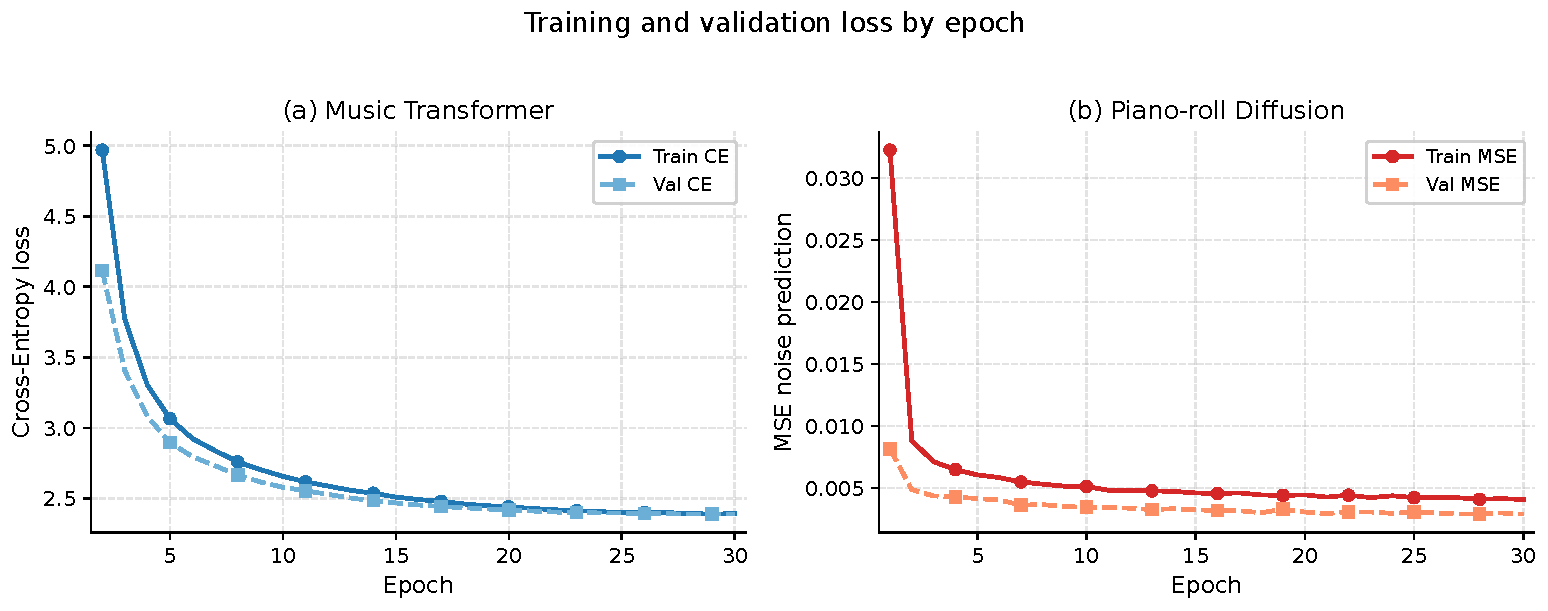
\includegraphics[width=0.88\textwidth]{fig_loss_by_epoch}
\caption{Đường cong hàm mất mát theo epoch của hai nhánh (huấn luyện/kiểm định). Lưu ý: entropy chéo và MSE không cùng thang đo, chỉ dùng để theo dõi hội tụ nội tại từng nhánh.}
\label{fig:ch4-loss-curves}
\end{figure}

\begin{figure}[htbp]
\centering
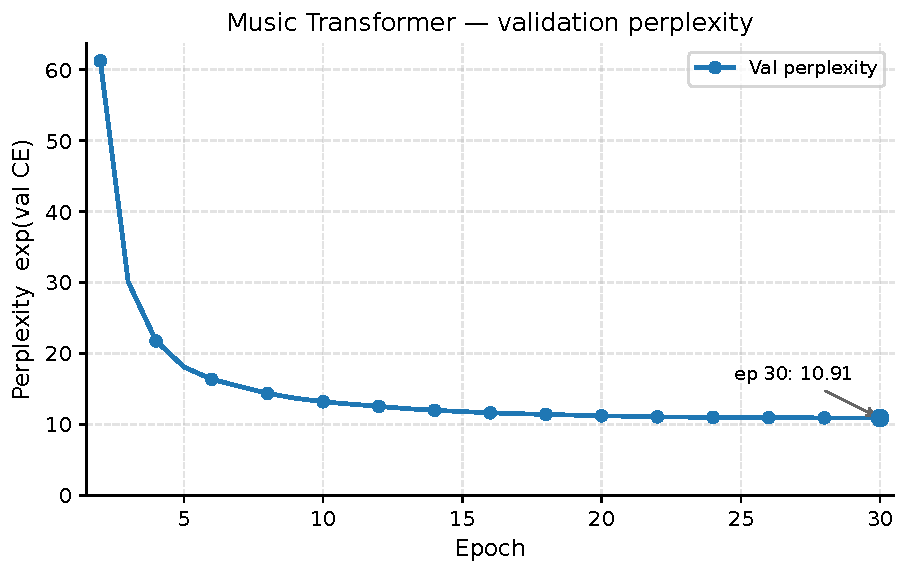
\includegraphics[width=0.75\textwidth]{fig_transformer_perplexity}
\caption{Độ bối rối kiểm định của Music Transformer theo epoch (thực nghiệm chính).}
\label{fig:ch4-tf-ppl}
\end{figure}

%------------------------------------------------------------------------------
\section{Chất lượng MIDI theo epoch (RQ2)}
\label{sec:ch4-quality}

Các chỉ số chất lượng lấy từ \texttt{quality\_summary.csv}, trung bình trên 20 tệp ứng với 20 prompt cho mỗi cặp phương pháp$\times$epoch.

\begin{table}[htbp]
\centering
\caption{Chỉ số MIDI trung bình (20 prompt) --- Transformer}
\label{tab:ch4-q-tf}
\scriptsize
\begin{tabular}{ccccccc}
\toprule
Ep & Số nốt & Mật độ & Đa âm & Im lặng & Khớp NC & Rỗng \\
\midrule
1 & 21.2 & 1.57 & 6.92 & 0.190 & 0.150 & 0.00 \\
5 & 35.9 & 6.15 & 2.84 & 0.401 & 0.176 & 0.15 \\
10 & 35.4 & 2.79 & 2.72 & 0.475 & 0.211 & 0.05 \\
20 & 40.9 & 3.66 & 1.87 & 0.371 & 0.278 & 0.10 \\
30 & 42.4 & 5.56 & 2.01 & 0.337 & 0.368 & 0.05 \\
\bottomrule
\end{tabular}
\end{table}

\begin{table}[htbp]
\centering
\caption{Chỉ số MIDI trung bình (20 prompt) --- Diffusion}
\label{tab:ch4-q-diff}
\scriptsize
\begin{tabular}{ccccccc}
\toprule
Ep & Số nốt & Mật độ & Đa âm & Im lặng & Khớp NC & Rỗng \\
\midrule
1 & 963 & 90.3 & 79.0 & 0.009 & 1.000 & 0.00 \\
5 & 1309 & 122.7 & 72.0 & 0.009 & 1.000 & 0.00 \\
10 & 1323 & 124.0 & 61.2 & 0.010 & 1.000 & 0.00 \\
20 & 1325 & 124.3 & 49.6 & 0.011 & 1.000 & 0.00 \\
30 & 920 & 86.3 & 42.6 & 0.009 & 1.000 & 0.00 \\
\bottomrule
\end{tabular}
\end{table}

Bảng~\ref{tab:ch4-q-ref} bổ sung sai lệch mật độ so với tham chiếu, khoảng cách JS trên pitch-class, và thời gian suy luận trung bình mỗi mẫu.

\begin{table}[htbp]
\centering
\caption{Sai lệch so với tham chiếu và JS pitch-class (trung bình)}
\label{tab:ch4-q-ref}
\scriptsize
\begin{tabular}{llccc}
\toprule
Phương pháp & Ep & Sai số mật độ & JS pitch-class & Suy luận (s/mẫu) \\
\midrule
Transformer & 1 & 3.86 & 0.179 & 3.90 \\
Transformer & 5 & 6.33 & 0.112 & 5.14 \\
Transformer & 10 & 4.22 & 0.155 & 4.29 \\
Transformer & 20 & 3.97 & 0.181 & 4.10 \\
Transformer & 30 & 4.77 & 0.149 & 4.08 \\
Diffusion & 1 & 85.4 & 0.074 & 2.49 \\
Diffusion & 5 & 117.8 & 0.075 & 2.57 \\
Diffusion & 10 & 119.1 & 0.080 & 2.64 \\
Diffusion & 20 & 119.5 & 0.080 & 2.49 \\
Diffusion & 30 & 81.4 & 0.082 & 2.35 \\
\bottomrule
\end{tabular}
\end{table}

\begin{figure}[htbp]
\centering
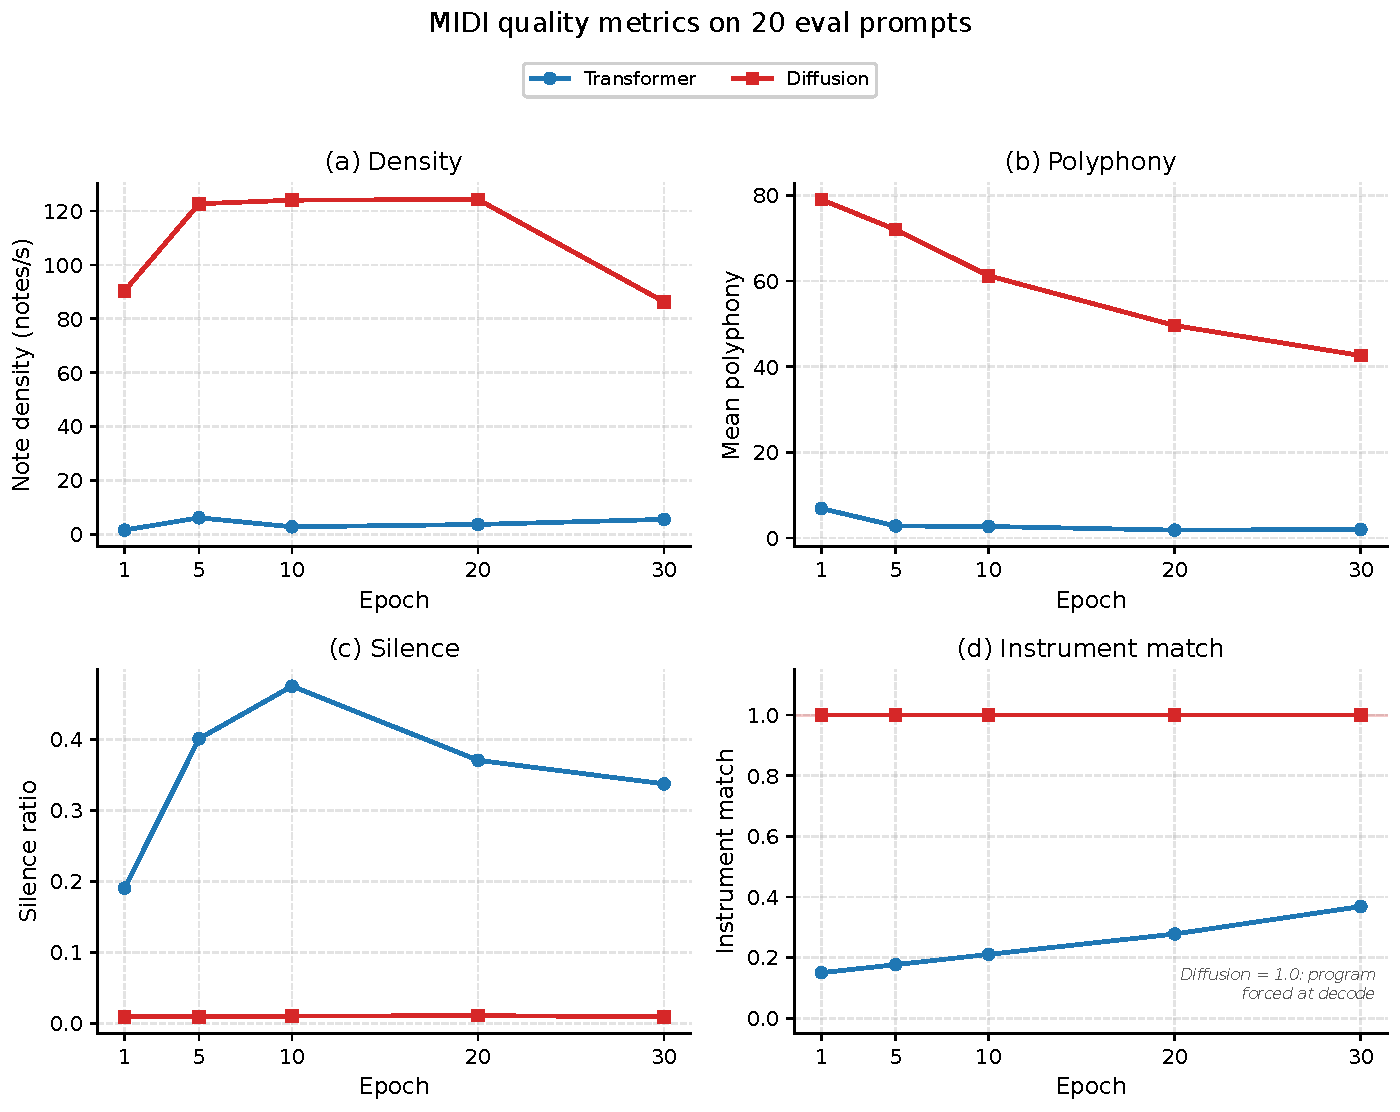
\includegraphics[width=0.88\textwidth]{fig_quality_metrics}
\caption{Một số chỉ số chất lượng MIDI trung bình theo epoch (hai nhánh). Cần đọc kèm lưu ý về \texttt{instrument\_match} ở nhánh Diffusion (Mục~\ref{sec:ch3-diff-decode}).}
\label{fig:ch4-quality-metrics}
\end{figure}

\begin{figure}[htbp]
\centering
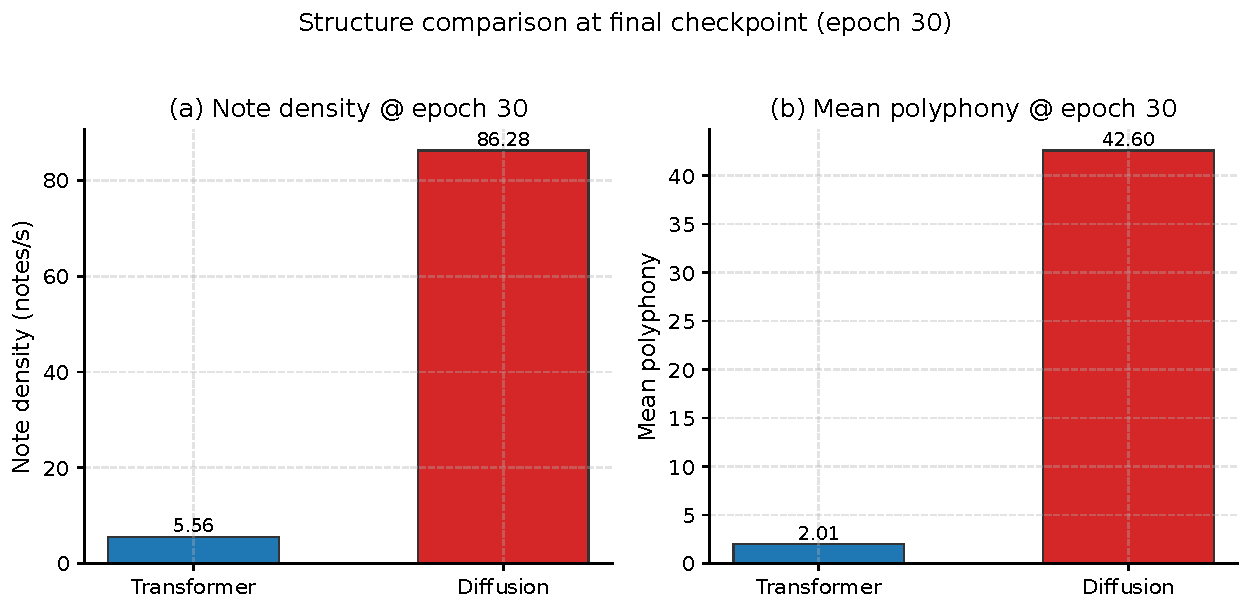
\includegraphics[width=0.78\textwidth]{fig_density_polyphony_ep30}
\caption{Đối chiếu mật độ nốt và đa âm trung bình tại epoch 30.}
\label{fig:ch4-density-poly-ep30}
\end{figure}

\subsection{Đọc kết quả phía Transformer}

Trên nhánh Transformer, số nốt trung bình tăng từ khoảng 21 lên 42, trong khi đa âm giảm từ $6.9$ ở epoch 1 về quanh $2$. Xu hướng này gần với cấu trúc thưa, kiểu giai điệu--hòa âm vừa phải, hơn là tập hợp nốt dày đặc. \texttt{instrument\_match} tăng từ \textbf{0.150} lên \textbf{0.368}, phù hợp việc mô hình dần sinh token/program khớp nhóm prompt hơn --- và vì giải mã lấy program từ token, chỉ số này phản ánh hành vi học. Tỉ lệ im lặng vẫn cao ($0.19$--$0.48$) và tỉ lệ mẫu rỗng dao động $0.05$--$0.15$ ở vài mốc, gợi ý sinh thiếu (\textit{under-generation}) hoặc dừng sớm hơn là overfitting theo hướng tăng mật độ nốt quá mức. Pitch-class JS tốt nhất trong các mốc báo cáo rơi vào epoch 5 ($0.112$), không đơn điệu theo entropy chéo kiểm định; nói cách khác, khả năng dự đoán token và độ gần phân bố pitch-class không phải một đường thẳng.

\subsection{Đọc kết quả phía Diffusion}

Diffusion cho kết quả khác biệt rõ. Mật độ nằm trong khoảng 86--124 nốt/giây và đa âm 43--79, lệch rất xa cả Transformer lẫn tham chiếu theo \texttt{note\_density\_abs\_err} (81--119). Tỉ lệ im lặng khoảng $0.009$ nghĩa là trên lưới thời gian gần như luôn có nốt. \texttt{instrument\_match} giữ \textbf{1.0} mọi epoch, kèm \texttt{num\_instruments}${}=1$ trong tóm tắt, khớp chính xác với việc \texttt{generate.py} gán \texttt{PROGRAM\_MAP} theo prompt (Mục~\ref{sec:ch3-diff-decode}). Con số này không được đọc như bằng chứng CFG đã học instrument hoàn hảo. Đa âm giảm từ 79 xuống 43 khi huấn luyện lâu hơn cho thấy việc giảm MSE có ảnh hưởng tới mức kích hoạt dày đặc của roll, nhưng epoch 30 vẫn còn đa âm $42.6$, chưa về vùng thưa. JS pitch-class của Diffusion thấp hơn Transformer ($0.07$--$0.08$) trong khi sai số mật độ vẫn lớn: histogram lớp nốt có thể gần tham chiếu theo tần suất tương đối mà vẫn không phản ánh mật độ hay đa âm hợp lý.

% Gợi ý hình piano-roll mẫu (cùng prompt, TF vs DF) có thể bổ sung sau từ
% compare/outputs; hiện tại khác biệt mật độ/đa âm đã thể hiện ở
% Hình~\ref{fig:ch4-density-poly-ep30} và các bảng chỉ số.

\subsection{Tóm tắt RQ2}

Trên cùng 20 prompt, Transformer cho MIDI thưa hơn, đa âm thấp hơn, và instrument\_match cải thiện theo quá trình học. Diffusion cho MIDI rất dày, còn instrument\_match bão hòa vì hậu xử lý. Khoảng cách đó nhất quán với thiên kiến quy nạp REMI kèm entropy chéo so với roll gộp kèm MSE và ngưỡng đã phân tích ở các chương trước; nó không mâu thuẫn với việc cả hai hàm mất mát đều giảm.

%------------------------------------------------------------------------------
\section{Chi phí tính toán (RQ3)}
\label{sec:ch4-cost}

\begin{table}[htbp]
\centering
\caption{Chi phí xấp xỉ từ nhật ký (thực nghiệm chính)}
\label{tab:ch4-cost}
\begin{tabular}{lcc}
\toprule
 & Transformer & Diffusion \\
\midrule
Số tham số & 7.72\,M & 4.43\,M \\
Đỉnh VRAM (nhật ký epoch) & $\approx 302$\,MB & $\approx 304$\,MB \\
Thời gian / epoch (ổn định) & $\approx 566$--570\,s & $\approx 1407$--1578\,s \\
Tích lũy 30 epoch (nhật ký) & $\approx 4.68$\,h (từ chuỗi ep2--30) & $\approx 12.57$\,h \\
Suy luận / mẫu (đánh giá) & $\approx 3.9$--5.1\,s & $\approx 2.4$--2.6\,s \\
Độ dài đoạn mặc định đánh giá & theo chuỗi/EOS (TB $\sim$17--30\,s tùy ep) & $\approx 10.67$\,s cố định \\
\bottomrule
\end{tabular}
\end{table}

\begin{figure}[htbp]
\centering
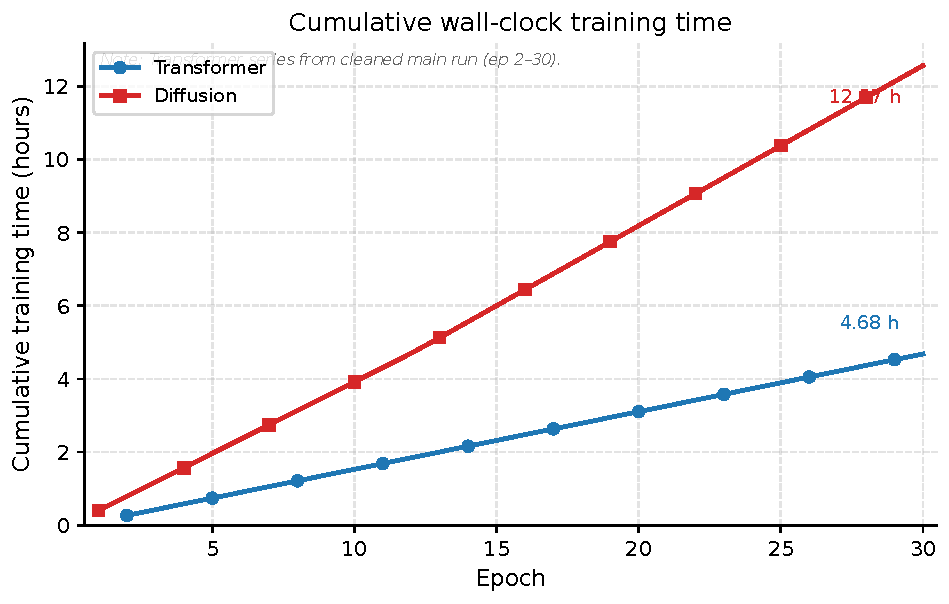
\includegraphics[width=0.78\textwidth]{fig_cumulative_train_time}
\caption{Thời gian huấn luyện tích lũy theo epoch (hai nhánh, thực nghiệm chính).}
\label{fig:ch4-cum-time}
\end{figure}

Diffusion có ít tham số hơn nhưng chậm huấn luyện rõ rệt: mỗi epoch trong nhật ký dài gấp khoảng $2{,}5$--$3$ lần Transformer, phù hợp chi phí UNet hai chiều và nhiều bước nhiễu khi học. Về suy luận, Diffusion nhanh hơn trên mỗi tệp đánh giá, song đoạn mặc định ngắn hơn và chỉ gồm 80 bước DDIM; Transformer chịu chi phí vòng tự hồi quy theo token và độ dài linh hoạt hơn. Đỉnh VRAM trong CSV quanh 300\,MB trông thấp so với quan sát thực dụng khi batch lớn. Đây là giá trị nhật ký đã ghi, có thể phản ánh bộ nhớ đã cấp phát tại thời điểm đo hơn là trần toàn tiến trình; khi tái lập nên đối chiếu \texttt{nvidia-smi} thay vì suy diễn thêm ngoài số liệu.

Trong ràng buộc GPU phổ thông của đồ án, Transformer tiết kiệm hơn về thời gian thực cho 30 epoch đã ghi; Diffusion tốn huấn luyện hơn dù số tham số nhỏ hơn. Suy luận Diffusion cạnh tranh về giây mỗi mẫu trên đoạn khoảng 10 giây. Nếu chỉ nhìn số tham số, sự đánh đổi sẽ bị diễn giải lệch.

%------------------------------------------------------------------------------
\section{Đối chiếu hai nhánh tại epoch 30}
\label{sec:ch4-ep30}

Bảng~\ref{tab:ch4-ep30} gom các chỉ số đã trích tại điểm kiểm tra cuối của giao thức so sánh, không phát sinh chỉ số mới ngoài CSV. Nó đóng vai trò tóm tắt tại thời điểm kết thúc huấn luyện; phần diễn giải chi tiết nằm ở các mục trước và Mục~\ref{sec:ch4-discussion}.

\begin{table}[htbp]
\centering
\caption{Tóm tắt epoch 30 (số liệu từ nhật ký/tóm tắt chất lượng)}
\label{tab:ch4-ep30}
\begin{tabular}{lcc}
\toprule
Chỉ số & Transformer & Diffusion \\
\midrule
Hàm mất mát huấn luyện & 2.392 (CE) & 0.00408 (MSE) \\
Hàm mất mát kiểm định & 2.389 (CE) & 0.00289 (MSE) \\
PPL (kiểm định) & 10.91 & -- \\
Số nốt (TB) & 42.4 & 920 \\
Mật độ (TB) & 5.56 & 86.3 \\
Đa âm (TB) & 2.01 & 42.6 \\
Im lặng (TB) & 0.337 & 0.009 \\
Khớp nhạc cụ & 0.368 & 1.000$^{\dagger}$ \\
Mẫu rỗng (TB) & 0.05 & 0.00 \\
Sai số mật độ vs tham chiếu & 4.77 & 81.4 \\
Suy luận (s/mẫu) & 4.08 & 2.35 \\
Số tham số (M) & 7.717 & 4.433 \\
\bottomrule
\multicolumn{3}{l}{\footnotesize $^{\dagger}$ Program gán từ prompt khi giải mã (xem Chương~\ref{chap:implementation}).}
\end{tabular}
\end{table}

%------------------------------------------------------------------------------
\section{Thảo luận tổng hợp và sự đánh đổi}
\label{sec:ch4-discussion}

\subsection{Hàm mất mát tốt không đồng nghĩa MIDI phù hợp mục tiêu ứng dụng}

Diffusion đạt MSE kiểm định khoảng $0.0029$ nhưng sai số tuyệt đối của mật độ vẫn trên 80. Transformer với entropy chéo kiểm định khoảng $2.39$ và độ bối rối khoảng $10.9$ lại đi kèm mật độ đơn vị và đa âm quanh 2. Khoảng cách đó khẳng định điều đã đặt ở Chương~\ref{chap:theory}: hàm mục tiêu học và chỉ số ứng dụng có thể phân kỳ, nhất là khi còn bước giải mã rời rạc nằm ngoài gradient.

\subsection{Vì sao Transformer cho cấu trúc sự kiện khả dĩ hơn?}

Ba quan sát trong phần triển khai và số liệu cùng chỉ một hướng. REMI buộc mô hình quyết định từng sự kiện nốt; entropy chéo phạt token sai và, nếu dữ liệu thưa, khuyến khích phân phối thưa. Đa âm cùng số nốt trong bảng~\ref{tab:ch4-q-tf} nằm ở thang đoạn nhạc có cấu trúc thưa hơn là phủ kín lưới. Instrument\_match tăng theo epoch cho thấy cross-attention kèm token \texttt{INST\_*} mang tín hiệu học đo được. Điểm yếu đi kèm cũng rõ: tỉ lệ im lặng và mẫu rỗng cho thấy đầu ra đôi khi còn thưa, chưa đủ dày nếu mục tiêu là BGM mật độ cao.

\subsection{Vì sao Diffusion vẫn dày dù đã có CFG, EMA và cosine schedule?}

Đối chiếu mã nguồn cho một chuỗi giải thích hợp lý hơn là gán nguyên nhân đơn lẻ cho ``chưa huấn luyện đủ''. Roll một kênh gộp track, kết hợp gamma làm nổi nốt nhẹ khi mã hóa, tạo mục tiêu vốn đã dễ dày. MSE không có hạng tử thưa hóa. \texttt{pianoroll\_to\_midi} với ngưỡng và cơ chế dự phòng hạ ngưỡng thiên về giữ nốt hơn là cắt bớt. CFG với $s=3.5$ có thể khuếch đại kích hoạt, nhưng CSV hiện tại không có phân tích loại trừ theo $s$, nên báo cáo chỉ ghi nhận cấu hình đã dùng chứ không khẳng định CFG là nguyên nhân duy nhất. Việc đa âm giảm theo epoch chứng minh huấn luyện có tác động; tác động đó chưa đủ để đưa mật độ về gần tham chiếu.

\subsection{Hạn chế diễn giải của chỉ số instrument\_match}

Đây là điểm phản biện then chốt của đồ án. Cùng một tên cột trong CSV, phía Transformer đo việc học sinh token/program, phía Diffusion đo quy trình gán program theo prompt. Mọi bảng xếp hạng mức tuân thủ instrument nếu bỏ chú thích này đều sai về phương pháp, dù con số trông có vẻ thuận lợi.

\subsection{Khi nào nghiêng về từng hướng?}

Trong phạm vi kết quả đã có, Transformer phù hợp hơn khi cần MIDI thưa, đa âm thấp, và muốn theo dõi hoặc điều khiển instrument qua sinh token, với chi phí đi kèm là tỉ lệ im lặng cao hơn và vẫn phụ thuộc EOS. Diffusion ở trạng thái hiện tại hợp lý hơn như đường cơ sở khử nhiễu trên roll và nền để cải thiện giải mã/hàm mất mát; nếu chỉ dựa mật độ và đa âm đã đo, chưa nên xem nó là lựa chọn BGM chính. Vì chưa có thử nghiệm nghe, báo cáo cũng không kết luận bên nào có chất lượng nghe cao hơn.

%------------------------------------------------------------------------------
\section{Hạn chế của đồ án}
\label{sec:ch4-limitations}

Một loạt giới hạn cần được nêu trung thực. Đồ án chưa có MOS, thử nghiệm nghe A/B, FAD hay CLAP score. Điều kiện text đã được hỗ trợ, nhưng caption huấn luyện chủ yếu theo template từ sáu nhãn (miền diễn đạt hẹp), MiniLM đóng băng (không fine-tune miền nhạc), và $c$ vẫn chỉ một vector toàn cục. Một phần nhãn có thể đến từ siêu dữ liệu hoặc heuristic nên mang nhiễu. Thời lượng đánh giá không khớp hoàn hảo giữa hai nhánh. Phía Diffusion, program bị gán cố định từ nhãn instrument; quy mô tham số thực nghiệm chính $4.43$\,M cũng khác một số lần thử $13.7$\,M. Phía Transformer, epoch 1 trong \texttt{comparison\_table} từng có kiểm định \texttt{nan} (lần chạy lỗi hoặc ghi đè) và đã bị loại khi phân tích hội tụ. Chưa có đường cơ sở ngoài kho mã nguồn (MIDI ngẫu nhiên, truy xuất theo nhãn, mô hình theo bài báo) và chưa phân tích loại trừ có hệ thống trên hệ số CFG, ngưỡng, làm mượt nhãn, độ dài chuỗi hay chất lượng caption.

%------------------------------------------------------------------------------
\section{Hướng phát triển}
\label{sec:ch4-future}

Các hướng dưới đây xuất phát trực tiếp từ hạn chế đã quan sát trong mã nguồn và số liệu, chứ không phải danh sách cải tiến chung chung. Với Diffusion, có thể thêm ràng buộc thưa hóa hoặc biểu diễn onset--frame hai kênh, chỉnh ngưỡng chống mật độ quá cao, và bỏ gán cố định program nếu muốn chỉ số instrument công bằng --- hoặc tách hẳn chỉ số ``program bị gán'' khỏi bảng so sánh. Với Transformer, hàm mất mát phụ cho \texttt{INST\_*}, tinh chỉnh lấy mẫu để giảm mẫu rỗng, và thử điều kiện đa token (chuỗi embedding từ MiniLM thay vì một vector gộp) là các bước gần. Về tầng text, đa dạng hóa template/caption, thử encoder nhạc--ngôn ngữ (CLAP) hoặc partial fine-tune projection sâu hơn, và đánh giá bám prompt ngoài tập câu chuẩn, sẽ làm rõ giới hạn MiniLM đóng băng. Về đánh giá, một thử nghiệm nghe nhỏ có kiểm soát, FAD/CLAP khi render audio thống nhất, và thống kê mật độ tham chiếu từ tập huấn luyện sẽ làm dày phần diễn giải. Về dữ liệu và huấn luyện, lọc piano/game sạch hơn, cân nhãn instrument, thêm lịch learning rate cho Diffusion, và thử lại UNet lớn hơn dưới cùng giải mã nếu VRAM cho phép, đều là mở rộng có căn cứ.

%------------------------------------------------------------------------------
\section{Trả lời tóm tắt các câu hỏi nghiên cứu}
\label{sec:ch4-rq-answers}

\textbf{RQ1.} Cả hai nhánh hội tụ ổn định trên hàm mục tiêu riêng: Transformer entropy chéo kiểm định về $2.389$, độ bối rối về $10.91$; Diffusion MSE kiểm định về $0.00289$. Huấn luyện và kiểm định của Transformer bám sát nhau; Diffusion không overfit theo nghĩa kiểm định tăng đột biến. Hai hàm mất mát không được so sánh chéo.

\textbf{RQ2.} Các chỉ số MIDI phân kỳ mạnh. Transformer thưa, đa âm quanh 2, instrument\_match tăng tới khoảng $0.37$. Diffusion dày (mật độ khoảng 86--124), đa âm 43--79, instrument\_match bằng $1.0$ do giải mã. Khác biệt truy về REMI+entropy chéo+token instrument đối lập roll+MSE+ngưỡng+\texttt{PROGRAM\_MAP}.

\textbf{RQ3.} Transformer mất khoảng $4.7$ giờ cho chuỗi 30 epoch đã ghi; Diffusion khoảng $12.6$ giờ. Suy luận Diffusion khoảng $2.4$ giây mỗi mẫu so với khoảng $4$ giây của Transformer, kèm khác biệt độ dài đoạn. Số tham số Diffusion nhỏ hơn nhưng huấn luyện tốn hơn trong thực nghiệm này.

%------------------------------------------------------------------------------
\section*{Tóm tắt chương}
\addcontentsline{toc}{section}{Tóm tắt chương}

Chương~\ref{chap:experiments} đã nối thiết lập thực nghiệm với hội tụ hàm mất mát, chỉ số MIDI, chi phí, thảo luận sự đánh đổi, hạn chế và hướng phát triển. Kết luận trung tâm có thể tóm tắt như sau: cả hai mô hình học tốt hàm mất mát của mình, nhưng trên giao thức MIDI hiện tại, nhánh Transformer cho cấu trúc sự kiện khả dĩ hơn, trong khi nhánh Diffusion cần cải thiện biểu diễn và giải mã trước khi có thể so sánh chất lượng BGM một cách công bằng về mật độ và, về lâu dài, về cảm nhận nghe.



\chapter*{Kết luận}
\addcontentsline{toc}{chapter}{Kết luận}
\setcounter{section}{0}
\renewcommand*{\thesection}{\the\value{section}}

Báo cáo đã triển khai và so sánh hai hệ sinh MIDI có điều kiện --- Music Transformer và Piano-roll Diffusion --- trên cùng quy trình dữ liệu, cùng pipeline mã hóa câu tiếng Anh (MiniLM đóng băng + lớp chiếu; projection học riêng từng nhánh), cùng kho đã xử lý và cùng mô-đun đánh giá. Sáu thuộc tính có cấu trúc vẫn đóng vai trò gán nhãn, sinh chú thích huấn luyện và meta chỉ số. Các câu hỏi nghiên cứu về hội tụ hàm mất mát, chất lượng cấu trúc MIDI và chi phí tính toán đã được trả lời dựa trên nhật ký huấn luyện và các chỉ số khách quan, trong điều kiện chưa thực hiện đánh giá cảm nhận nghe có kiểm soát.

\subsection*{Kết quả đạt được}

\begin{enumerate}
    \item Xây dựng đặc tả đầu vào--đầu ra thống nhất (câu English $\rightarrow$ MIDI) và quy trình dữ liệu dùng chung (khoảng 14\,232 tệp MIDI; phân chia 12\,809/1\,423), kèm cầu nối nhãn sáu thuộc tính $\rightarrow$ chú thích tiếng Anh.
    \item Hiện thực hóa theo quy trình đầu cuối hai nhánh tạo sinh (REMI kết hợp Transformer và piano-roll kết hợp UNet diffusion), với pipeline \texttt{TextPromptEncoder} dùng chung (projection học riêng), kèm huấn luyện, lưu điểm kiểm tra (\textit{checkpoint}) và sinh mẫu.
    \item Thiết lập giao thức đánh giá có thể tái lập (20 câu prompt chuẩn, chỉ số cấu trúc MIDI, ghi nhận thời gian, bộ nhớ GPU và số tham số).
    \item Quan sát thực nghiệm chính: cả hai nhánh hội tụ tốt trên hàm mục tiêu riêng; Transformer cho đa âm và mật độ thưa hơn, chỉ số khớp nhạc cụ tăng theo quá trình học; Diffusion đạt MSE thấp nhưng mật độ và đa âm cao, chỉ số khớp nhạc cụ bằng $1{,}0$ gắn với bước gán chương trình nhạc cụ sau sinh.
    \item Làm rõ sự đánh đổi phương pháp: không so sánh trực tiếp entropy chéo với MSE; mọi chỉ số cần được diễn giải gắn với chi tiết triển khai tương ứng.
\end{enumerate}

\subsection*{Hạn chế}

\begin{enumerate}
    \item Chưa có đánh giá cảm nhận (MOS, thử nghiệm A/B) hay chỉ số phân phối trên audio (FAD, CLAP).
    \item Câu điều kiện huấn luyện chủ yếu sinh từ mẫu template trên sáu nhãn (chưa đa dạng hóa diễn đạt); backbone MiniLM đóng băng nên không tinh chỉnh miền nhạc; vector điều kiện vẫn được nén thành một token/$c$ toàn cục.
    \item Nhánh Diffusion dùng piano-roll một kênh; bước ngưỡng hóa và gán chương trình nhạc cụ cố định làm lệch một số chỉ số so sánh.
    \item Chưa thực hiện phân tích loại trừ (\textit{ablation}) đầy đủ và chưa có đường cơ sở (\textit{baseline}) ngoài kho mã nguồn của đồ án.
\end{enumerate}

\subsection*{Hướng phát triển}

\begin{enumerate}
    \item Cải thiện nhánh Diffusion theo hướng thưa hóa / biểu diễn onset--frame và quy trình giải mã; tách chỉ số chương trình nhạc cụ bị gán cố định khỏi bảng so sánh công bằng.
    \item Nâng cao điều kiện hóa text: đa dạng hóa caption, thử CLAP/encoder nhạc--ngôn ngữ, hoặc nhiều token điều kiện; bổ sung hàm mất mát phụ cho nhạc cụ ở nhánh Transformer.
    \item Bổ sung đánh giá cảm nhận quy mô nhỏ và thống kê tham chiếu từ tập huấn luyện.
    \item Mở rộng dữ liệu đã lọc theo miền game/piano khi điều kiện tài nguyên cho phép.
\end{enumerate}

Tóm lại, giá trị của báo cáo nằm ở \textbf{thực nghiệm so sánh thống nhất} và \textbf{phân tích trung thực} giữa hai thiên kiến quy nạp (\textit{inductive bias}) tạo sinh trên bài toán MIDI có điều kiện bằng text ở quy mô đồ án tốt nghiệp, chứ không nằm ở tuyên bố vượt các hệ text-to-music thương mại.


\addtocontents{toc}{\protect\setcounter{tocdepth}{0}}
\setcounter{section}{0}
\renewcommand*{\thesection}{\the\value{section}}
\begin{thebibliography}{99}\rm
\addcontentsline{toc}{chapter}{\bfseries Tài liệu tham khảo}

\bibitem{vaswani2017attention}
A.~Vaswani et al., \textit{Attention is All You Need}, NeurIPS, 2017.

\bibitem{huang2018music}
C.-Z.~A.~Huang et al., \textit{Music Transformer: Generating Music with Long-Term Structure}, ICLR, 2019.

\bibitem{ho2020ddpm}
J.~Ho, A.~Jain, and P.~Abbeel, \textit{Denoising Diffusion Probabilistic Models}, NeurIPS, 2020.

\bibitem{song2021ddim}
J.~Song, C.~Meng, and S.~Ermon, \textit{Denoising Diffusion Implicit Models}, ICLR, 2021.

\bibitem{nichol2021improved}
A.~Q.~Nichol and P.~Dhariwal, \textit{Improved Denoising Diffusion Probabilistic Models}, ICML, 2021.

\bibitem{ho2022cfg}
J.~Ho and T.~Salimans, \textit{Classifier-Free Diffusion Guidance}, NeurIPS Workshop on Deep Generative Models, 2021.

\bibitem{holtzman2020curious}
A.~Holtzman et al., \textit{The Curious Case of Neural Text Degeneration}, ICLR, 2020.

\bibitem{agostinelli2023musiclm}
A.~Agostinelli et al., \textit{MusicLM: Generating Music From Text}, arXiv:2301.11325, 2023.

\bibitem{copet2023musicgen}
J.~Copet et al., \textit{Simple and Controllable Music Generation} (MusicGen), NeurIPS, 2023.

\bibitem{liu2023audioldm}
H.~Liu et al., \textit{AudioLDM: Text-to-Audio Generation with Latent Diffusion Models}, ICML, 2023.

\bibitem{hawthorne2018maestro}
C.~Hawthorne et al., \textit{Enabling Factorized Piano Music Modeling and Generation with the MAESTRO Dataset}, ICLR, 2019.

\bibitem{commu2023}
H.~Lee et al., \textit{ComMU: Dataset for Combinatorial Music Generation}, NeurIPS Datasets and Benchmarks, 2022.

\end{thebibliography}

\end{document}
